%!TEX TS-program = xelatex
%!TEX encoding = UTF-8 Unicode

\documentclass{harvard-thesis}

%\usepackage{astron}
%\usepackage{polski}
%\usepackage[utf8]{inputenc}
\usepackage[polish]{babel}
%\usepackage[T1]{fontenc}

%%%%%%%%%%%%%%%%%%%%%%%%%%%%%%%%%%%%%%%%%%%%%%%%%%%%%%%%%%%%%%%%%%%%%%%%
%%% LaTeX Package Summary (http://trackchanges.sourceforge.net/)
%%% The trackchanges.sty style file adds five new LaTeX comands commands:
%%% \note[editor]{The note}
%%% \annote[editor]{Text to annotate}{The note}
%%% \add[editor]{Text to add}
%%% \remove[editor]{Text to remove}
%%% \change[editor]{Text to remove}{Text to add}
%%%
%%% In all cases [editor] can be ommitted.
%%%
%%% All of the TrackChanges commands allow for the specification of an editor. Specifing an editor will prefix the edits with the editor name and color code their changes in the final pdf or dvi file.
%%%
%%% To specify an editor name, the editor must first be declared in the preamble:
%%% \addeditor{editor one}
%%% \addeditor{editor two}
%%%
%%% Display Options
%%% Track changes has a number of different ways that it can display the edits in the final dvi or pdf file.
%%% finalold  - Reject all edits.
%%% finalnew  - Accept all edits.
%%% footnotes - Display edits as footnotes.
%%% margins   - Display edits as margin notes.
%%% inline    - Display edits inline.
%%%
%%% See the Documentation for additional options.
%%% Examples with the differnt display options can be found on the Preview page.
%%%%%%%%%%%%%%%%%%%%%%%%%%%%%%%%%%%%%%%%%%%%%%%%%%%%%%%%%%%%%%%%%%%%%%%%
\usepackage[inline]{trackchanges}           %%% !!! USE THIS TO DISPLAY ALL CHANGES AND NOTES  !!!
\addeditor{MH}
\addeditor{KK}

\begin{document}

% the front matter
% some details about the thesis
%\title{Połączone działanie niestabilności płynowych w dyskach protoplanetarnych}
\title{Powstawanie planet w wyniku połączonego działania niestabilności płynowych w dyskach protoplanetarnych}
\author{Kacper Kowalik}
\advisor{prof. dr hab. Michał Hanasz}

% about the degree
\degree{Rozprawa doktorska}
\field{Astronomia}
\degreeyear{2014}
\degreemonth{wrzesień}

% about the university
\department{Katedrze Astronomii i Astrofizyki}
\university{Uniwersytet Mikołaja Kopernika}
\universitycity{Toruń}
\universitystate{}

\maketitle
\copyrightpage
\abstractpage
\tableofcontents
%\authorlist
\listoffigures
%\dedicationpage
\acknowledgments

\onehalfspacing

% include each chapter...
\begin{savequote}[75mm]
   You know nothing, Jon Snow.
\qauthor{Ygritte, A Song of Ice and Fire by George R. R. Martin}
\end{savequote}

\chapter{Wprowadzenie}
\newthought{Skąd wzięły się planety?} Pytanie, które nurtuje ludzkość od
zamierzchłych czasów. Konkretne rozważania teoretyczne dotyczące pochodzenia
planet mają długą historię sięgającą przynajmniej XVIII wieku, kiedy to Immanuel
Kant wysunął ,,Hipotezę mgławicową''~\cite{ImmanuelKant.etal:2008}. Już wtedy
unikalność Układu Słonecznego stanowiła przedmiot debaty. Dopiero na początku XX
wieku pogląd, iż układy planetarne są czymś powszechnym we Wszechświecie, został
zaakceptowany przez środowisko naukowe, a w~roku 1992 została odkryta pierwsza,
pozasłoneczna planeta orbitująca pulsar PSR 1257+12b~\cite{1992Natur.355..145W}.
Dziś znamy ponad 1800 układów planetarnych orbitujących gwiazdy znajdujące się
na różnorakich etapach ewolucji. Pomimo tego bogactwa danych obserwacyjnych
i~wieloletnich badań teoretycznych, odpowiedź na pytanie \emph{skąd wzięły się
planety} pozostaje niejednoznaczna.

%\begin{figure}[!ht]
%\centering
%\includegraphics[width=0.8\textwidth]{figures/laplace.png}
%\caption{Model mgławicy Laplace'a: (a) rotująca mgławica; (b) kolapsująca
%mgławica ulega spłaszczeniu wzdłuż osi rotacji; (c) soczewkowaty kształt
%mgławicy; (d) pierścienie materii pozostawione przez zapadający się obiekt
%centralny; (e) zagęszczenia na poszczególnych pierścieniach kolapsują tworząc
%planety. (Obrazek z~pracy Woolfson, 1993)} 
%\label{fig:laplace}
%\end{figure}

\section{Paradygmat powstawania planet}
\subsection{Narodziny gwiazdy}
Formowanie się planet jest nierozerwalnie związane z~narodzinami gwiazd, które
biorą swój początek w~gęstych pyłowo--gazowych obłokach materii. Zanurzone w
gorącym ośrodku międzygwiazdowym, początkowo w~stanie równowagi termodynamicznej
z otaczającym je gazem, obłoki takie często występują w~ogromnych kompleksach i
obserwowane są jako ciemne mgławice molekularne~\cite{Tielens05}. W~ich pobliżu
odnajdywane są gwiazdy~\emph{T Tauri} -- obiekty zmienne o jasności większej niż
wynikałoby to z~ich temperatur efektywnych, co sugeruje ich młody wiek,
nieprzekraczający 1~\Myr~\cite{H62}. Obserwowane temperatury efektywne sugerują,
iż we wnętrzach nie panują dostatecznie wysokie temperatury, aby mogły zachodzić
już reakcje spalania wodoru~\cite{CK79}. Część obserwowanych gwiazd T~Tauri jest
częściowo zanurzona w~małych, ciemnych i~gęstych obłokach materii. Jak pokazują
obserwacje na falach radiowych i~w~podczerwieni, obłoki te są na tyle gęste, że
siła wynikająca z gradientu ciśnienia jest w~stanie zrównoważyć siłę pochodzącą
od samograwitacji~\cite{WT02}. Ich wewnętrzna struktura jest wysoce
hierarchiczna, tzn. we wnętrzu pojedynczego gęstego obłoku o masach rzędu
tysięcy mas słonecznych rozciągającego się na wiele parseków, znajdują się dużo
gęstsze obiekty o masach rzędu $1\Msun$ i~rozmiarach rzędu $0.1\pc$~\cite{M85,
LSM93}. Obserwacje rotacyjnych linii emisyjnych molekuły NH$_3$ pozwalają
szacować typowe koncentracje gazu w~obłokach na $10^{4}\cm^{-3}$~\cite{BM89}.
Nieregularny brzeg obłoków, w~połączeniu z~ich w~przybliżeniu fraktalną
strukturą, interpretowany jest jako obecność silnej turbulencji w samych
obłokach~\cite{E00, FPW91}. Nie jest jasne czy ta struktura jest przejściowym
etapem ewolucji całego kompleksu obłoków, czy też quasi-stacjonarnym
stanem~\cite{L94}. Źródła turbulencji można upatrywać w supernowych, wiatrach
gwiazdowych, promieniowaniem masywnych gwiazd oraz niestabilnościach związanych
z polem magnetycznym~\cite{NP03, MLK04}. 
Typowe temperatury obłoków molekularnych wynoszą od
10 do 20\K. Za efektywne chłodzenie początkowo odpowiada emisja w~podczerwieni
molekuły CO~\cite{MSWG82}, jednakże w~trakcie kolapsu grawitacyjnego gaz sprzęga
się termicznie z~pyłem, który wypromieniowuje nadwyżkę energii
w~podczerwieni~\cite{HN65, MI00} przez co temperatura całego zapadającego się
obłoku pozostaje stała w czasie.

\par Procesy zachodzące w~samych obłokach tj. turbulencja, samograwitacja, lub
w ośrodku zewnętrznym tj.  wybuchy supernowych mogą powodować wzrost gęstości
poszczególnych zagęszczeń w~obłoku. W~momencie, w~którym obszar gęstej materii
przekroczy  masę krytyczną, nazywaną masą Jeansa $M_J$~\cite{J1902, J1928},
grawitacja przeważa i~chmura zaczyna się zapadać (rysunek 1a). Masa Jeansa
zależy od temperatury kinetycznej ośrodka $T$ oraz jego gęstości
$\rho$~\cite{H64}:
%
\begin{equation} M_J \sim
   \left( \frac{k_B T}{G} \right) ^\frac{3}{2} {\rho}^{-\frac{1}{2}},
\end{equation}
%
gdzie $k_B$ jest stałą Boltzmanna a $G$ jest stałą grawitacji.
Dla wymienionych powyżej typowych warunków panujących wewnątrz obłoków materii
międzygwiazdowej~\cite{BM89}, masa Jeansa przyjmuje wartość:
%
\begin{equation}
 M_J \approx 2.9 M_{\odot} \left(\frac{T}{10\K}\right)^{1.5} 
 \left(\frac{n}{10^4\cm^{-3}}\right)^{-0.5},
\end{equation}
%
gdzie $n = \rho_g / \mu \mH$ jest koncentracją cząstek materii.
Gdyby gradient ciśnienia był niewystarczający do utrzymania równowagi, kolaps
obłoku następowałby w~tzw. skali czasowej spadku swobodnego~\cite{Spitzer1978}:
%
\begin{equation}
   t_{\textrm{ff}} \sim \frac{1}{\sqrt{G\rho}} \sim 10^5\yr
   \left(\frac{n}{10^4\thinspace \cm^{-3}}\right)^{-0.5}.
\end{equation}
%
W~rzeczywistości gradient ciśnienia w~niewielkim tylko stopniu spowalnia
zapadanie się materii~\cite{T82}. Obliczenia numeryczne pokazują, że profil
gęstości materii w~zapadającym się, sferycznie symetrycznym obłoku, pozbawionym
pola magnetycznego i turbulencji, asymptotycznie zbiega do funkcji
proporcjonalnej do $r^{-2}$~\cite{L69}. W~rezultacie tylko niewielka część masy
obłoku formuje protogwiazdę, reszta materii zostaje uwięziona w~formie
rozciągniętej otoczki opadającej na obiekt centralny. Przy braku rotacji
i~zaniedbaniu wpływu pola magnetycznego otoczka opada radialnie w~tempie
proporcjonalnym do $c_s^3 / G$, gdzie $c_s$ jest izotermiczną prędkością
dźwięku.  Stała proporcjonalności wynosi od około jedności~\cite{S77} do
kilkudziesięciu~\cite{H77}.

\par Jak już wcześniej wspomniano, pole magnetyczne odgrywa istotną rolę w
dynamicznej ewolucji całego kompleksu obłoków molekularnych i~należy spodziewać
się obecności silnego pola magnetycznego w~zapadającym się obłoku molekularnym i
jego przeciwdziałania sile samograwitacji~\cite{MC99}. Jednym z możliwych
mechanizmów zapoczątkowujących kondensację materii w~centrum grawitacji jest
dyfuzja ambipolarna, która zachodzi w~skalach czasowych rzędu
$10^7$~lat~\cite{MZGH93}.  Dzięki stopniowemu zwiększaniu masy, centralna część
podtrzymywanego przez pole magnetyczne obłoku ulega powolnej kontrakcji do
momentu osiągnięcia koncentracji materii rzędu $10^{5}\cm^{-3}$, dla której
siła samograwitacji przeważa nad ciśnieniem magnetycznym i~rozpoczyna się
niepohamowany kolaps~\cite{BM94, CB00}. Niedawne eksperymenty
numeryczne~\cite{JHCF13} sugerują, że uwzględnienie wpływu turbulencji podczas
kolapsu pozwala efektywniej przełamać przeciwdziałający samograwitacji wpływ
pola magnetycznego, nawet dla silnie namagnesowanego ośrodka.

\par W powyższych rozważaniach całkowicie zaniedbano wpływ rotacji na ewolucję
formującej się protogwiazdy. Większość obserwowanych obłoków materii z której
formują się potem gwiazdy rotuje~\cite{GBFM93}, co wydaje się być naturalną
konsekwencją turbulencji obecnej w~obłokach~\cite{BB00}. Typowy moment pędu
szacowany w~obłokach protogwiazdowych jest przynajmniej o rząd większy niż
moment pędu, który posiadałaby gwiazda rotując z~maksymalną prędkością
równoważącą siłę samograwitacji. 

Fakt ten implikuje konieczność uwzględnienia mechanizmu odpowiedzialnego za
radialny transport momentu pędu Rotacja powoduje, że materia nie opada
centralnie na centrum grawitacji, lecz formuje dysk podtrzymywany przez
równowagę pomiędzy radialną składową siły grawitacji oraz siłę
odśrodkową~\cite{TSC84}. Biorąc pod uwagę masę opadającą z~otoczki, formujący
się dysk jest marginalnie stabilny, bądź jest całkowicie niestabilny
grawitacyjnie~\cite{SKBT94}. W~rezultacie tworzą się w~nim spiralne fale
gęstości, które pod wpływem momentu siły wynikającego z oddziaływania
grawitacyjnego porcji gazu tworzącego dysk, napędzają akrecję materii na
protogwiazdę~\cite{St00}.
Akrecja materii przebiega w sposób nie zaburzony jeżeli fluktuacje gęstości
wysycają się na odpowiednio niskim poziomie. W przeciwnym razie dysk może
rozpaść się tworząc układ podwójny lub wielokrotny.
%Ewolucja masywnego dysku zostanie dokładnie opisana w
%podrozdziale~\ref{sec:GI}. 

\par Formujące się w~centrum zagęszczenie staje się nieprzezroczyste dla
termicznej emisji pyłu przy gęstościach gazu większych niż $10^{-13}\g\cm^{-3}$
$(2\cdot10^{10}$ H$_2\cm^{-3})$~\cite{L69} w~wyniku czego temperatura wnętrza
obłoku zaczyna rosnąć. Kończy to etap izotermicznego kolapsu. Nieprzezroczyste
jądro obłoku staje się adiabatyczne (wykładnik adiabatyczny H$_2$: $\gamma =
7/5$~\cite{L69}) dla gęstości powyżej $10^{-12}\g\cm^{-3}$. W adiabatycznie
ściskanym gazie ciśnienie prowadzi do praktycznie
całkowitego zatrzymania kolapsu dla gęstości centralnej $\sim 2\cdot
10^{-10}\g\cm^{-3}$ w rezultacie gaz  osiąga równowagę hydrostatyczną. Gaz
z~otoczki nie przestaje być jednak akreaowany i gęstość oraz temperatura jądra
cały czas rośnie. Krytycznym momentem jest osiągnięcie przez gaz temperatury
$2000\K$, dla której następuje dysocjacja molekuły H$_2$ i~gwałtowny spadek
wykładnika adiabatycznego poniżej wartości $4/3$. Ta druga faza kolapsu zachodzi
podobnie jak początkowy kolaps izotermiczny. Faza ta trwa, aż do momentu kiedy
wodór zostanie zjonizowany przez wzrost temperatury i~wykładnik adiabatyczny
gazu wzrośnie do wartości $5/3$.  Wzrost ciśnienia prowadzi do uformowania
drugiego jądra pozostającego w równowadze hydrostatycznej. Posiada ono dość
niewielką masę rzędu $10^{-3}\Msun$ i~rozmiar około $1\Rsun$~\cite{MI00}.
Całkowita masa formującej się protogwiazdy nie przekracza na tym etapie
$10^{-2}\Msun$.  Dominującym procesem staje się akrecja materii, która musi
dostarczyć pozostałe 99\% masy do rodzącej się gwiazdy. 

W~trakcie akrecji, protogwiazda cały czas pozostaje niewidoczna dla obserwatora,
ponieważ jest przysłonięta przez pył znajdujący się w~opadającej otoczce.
Klasyfikacja obserwacyjna takiego układu określa obiekty na tym etapie mianem
\emph{klasy zero}~\cite{andre} (rysunek 1b). Ich obserwowana temperatura jest
stosunkowo niska $(T \lesssim 30\K)$. Obiekty te charakteryzują się maksimum
w~rozkładzie energii promieniowania wypadającym w~dalekiej podczerwieni, bez
wykrywalnej nadwyżki w~bliskiej podczerwieni. Z czasem kiedy z~otoczki ubywa
materii, obszar optycznie gruby staje się coraz mniejszy i~maksimum
wypromieniowywanej energii przesuwa się w~kierunku bliższej podczerwieni.
Ostatecznie światło samej gwiazdy przebija się przez pozostałość otoczki, dzięki
czemu można zaobserwować charakterystyczne, dwuskładnikowe widmo (patrz
Rysunek~\ref{fig:sed}). Obserwatorzy wprowadzili prostą klasyfikację tak młodych
obiektów dzieląc je na 4 klasy: 0, I, II i~III, które oznaczają położenie
maksimum w~rozkładzie energii promieniowania odpowiednio na falach:
submilimetrowych, dalekiej podczerwieni, bliskiej podczerwienie i~w~zakresie
widzialnym. Poszczególne klasy odpowiadają też różnym fazom akrecji materiału i
różnią się długością trwania. Protogwiazdy znajdują się w~klasie 0 przez około
kilkadziesiąt tysięcy lat~\cite{FSSK06}. W~tym czasie następuje gwałtowna
akrecja materii.  Klasa I jest o rząd wielkości dłuższa (kilka $10^5$ lat), zaś
maksymalny wiek obserwowanych gwiazd T Tauri (klasa II) wynosi $10^6$
lat~\cite{HCGD98}.  Dla obiektów klasy III w~widmach zanikają wszelkie struktury
przypisywane materii okołogwiazdowej~\footnote{ang. \emph{weak-line T Tauri
stars}}.  Protogwiazda traci materię z~dysku na skutek jego
fotoewaporacji~\cite{ACP06} i~wiatru gwiazdowego~\cite{PN86}. Wiele
obserwowanych gwiazd T Tauri wykazuje w~obserwowanych widmach już tylko
szczątkową akrecję $10^{-7} \div 10^{-8} \Msun\rok^{-1}$~\cite{Hart98}. Tak niski
poziom akrecji nie jest już w~stanie znacząco wpłynąć na masę gwiazdy i~proces
jej formowania można uznać za zakończony.

\subsection{Powstawanie planet}

Proces formowania się planet najprawdopodobniej nie jest pojedynczym procesem,
lecz złożeniem wielu różnych etapów, w~których każdy kolejny krok bazuje na
produktach poprzedniego. Już w~połowie XX wieku Carl von
Weizsacker~\cite*{1943ZA.....22..319W} i~Gerard
Kuiper~\cite*{1951PNAS...37....1K} zapostulowali, iż dynamiczna ewolucja obłoku
protoplanetarnego prowadzi do utworzenia się lokalnych zagęszczeń gazu i~pyłu.
Postulowany model zakłada, że mikroskopijne cząsteczki pyłu sklejają się ze sobą
tworząc coraz to większe ciała --- \emph{planetezymale}. Kiedy planetezymale
osiągną rozmiary $\sim 10\m$ ich wzajemne oddziaływanie grawitacyjne zaczyna
przeważać nad siłami tarcia aerodynamicznego. Następnie planetezymale zaczynają
się zderzać formując obiekty o rozmiarach rzędu tysięcy kilometrów ---
protoplanety. Protoplanety zaś są na tyle masywne, iż są w~stanie akreować
otaczający je gaz. Bardziej szczegółowo można podzielić formowanie się planet na
4 etapy:

\begin{description}
   \item[i) koagulacja ziaren pyłu $\left(\mum \rightarrow \km\right):$] 
      Z doświadczeń laboratoryjnych wynika~\cite{BW08}, że drob\-ne cząsteczki pyłu
      mogą na skutek wzajemnych zderzeń zwiększać swoje rozmiary. ,,Spoiwem'' stają
      się siły van der Waalsa bądź oddziaływanie elektrostatyczne. Opierając się
      na analizie drogi swobodnej jednorodnej frakcji cząstek pyłu o promieniu
      $a$, można określić charakterystyczną skalę czasową koagulacji jako 

   \begin{equation}\label{coag} 
      t_{\textrm{coag}} % = \frac{1}{n_d \sigma \Delta v}
      \sim \frac{a}{\Delta v}\frac{\rho_p}{\rho_d} \approx 
      10^{-12} \rho_d^{-1}\yr\thinspace
      \left(\frac{a}{1\mum}\right)
      \left(\frac{\Delta v}{0.1\m\s^{-1}}\right)^{-1}
      \left(\frac{\rho_p}{3\g\cm^{-3}}\right),
   \end{equation}

   gdzie $\Delta v$ jest średnią prędkością względna cząstek, $\rho_p$ jest
   gęstością materiału budującego cząstki natomiast $\rho_d$ jest gęstością
   ośrodka pyłowego w~dysku.  Biorąc pod uwagę typowe gęstości pyłu w~obłokach
   gwiazdowych $(\rho_d \sim 10^{-20}\g\cm^{-3})$ proces ten zachodzi w~skali
   czasowej milionów lat. Jednakże dla dysków protoplanetarnych o typowych
   gęstościach rzędu $10^{-10}\g\cm^{-3}$ (jest to całkowita gęstość z
   uwzględnieniem obu składników: gazu i~pyłu. Przyjmuje się że kanoniczna
   wartość stosunku gęstości pyłu do gęstości gazu $\epsilon$ wynosi
   0.01~\footnote{w rzeczywistości wartość ta nie jest znana. Przyjmuje się, że
   stosunek jest gęstości pyłu do gęstości gazu jest podobna jak ta obserwowana
   w~ośrodku międzygwiazdowym~\cite{FS03}}. Zatem $\rho_d \sim
   10^{-12}\g\cm^{-3}$) proces koagulacji zachodzi w~skalach lat czy tez
   dziesiątek lat i~może bardzo szybko prowadzić do wytworzenia się
   planetezymali. W~rzeczywistości dla ziaren pyłu o rozmiarach decymetrów czy
   metrów pojawia się szereg procesów przeciwdziałających dalszemu wzrostowi, a
   także ulega zmianie średnia prędkość względna cząstek pyłu zmieniając
   prawdopodobieństwo wyniku kolizji na korzyść fragmentacji raczej niż
   koagulacji. Szczegółowy opis tych procesów znajdzie się w kolejnych podrozdziałach.

\item[ii) oligarchiczny wzrost $\left(\km \rightarrow
   10^3\km\right)$:]
   Faza druga formowania się planet rozpoczyna się w~momencie w~którym przeważa
   wzajemne oddziaływanie grawitacyjne pomiędzy planetezymalami. Spoiwem
   łączącym zderzające się obiekty staje się grawitacja. W~trakcie bliskich
   przelotów (ang. \emph{close encounters}) mało masywne planetezymale doznają
   znacznych przyspieszeń przez co rosną ich prędkości względne, w
   przeciwieństwie do masywnych obiektów~\cite{WS93}. Dla ciał poruszających się z
   podobnymi prędkościami prawdopodobieństwo zderzenia jest większe, jako że
   grawitacja jest w~stanie zbliżyć ich trajektorie. W~rezultacie obiekty
   najmasywniejsze w~danym obszarze dysku przybierają na masie najszybciej i
   zaczynają dominować lokalną dynamikę wszystkich sąsiadujących
   planetezymali~\cite{IM93}. Ostatecznie w~poszczególnych obszarach dysku
   protoplanetarnego formuje się pojedynczy obiekt -- jądro protoplanetarne
   oraz pozostaje pewna populacja mniejszych planetezymali~\cite{KI98}. Jądra
   protoplanetarne są też nazywane ,,oligarchami'', a etap ten określany jest
   jako ,,oligarchiczny wzrost''.
   Tempo przyrostu masy oligarchów mocno zależy od typowych rozmiarów
   planetezymali, które pozostały w~dysku. Mniejsze ciała silnie oddziałują z
   gazem poprzez tarcie aerodynamiczne, które ukoławia ich orbity zwiększając
   równocześnie prawdopodobieństwo wychwytu przez pobliskie jądra
   protoplanetarne na skutek soczewkowania
   grawitacyjnego~\footnote{soczewkowanie grawitacyjne należy rozumieć jako
      zwiększenie przekroju czynnego na zderzenie, spowodowanego oddziaływaniem
   grawitacyjnym, ang. \emph{gravitational focusing}, nie zaś jako zakrzywienie
promieni świetlnych w~polu grawitacyjnym masywnego ciała ang.
\emph{gravitational lensing}.}~\cite{R04}.
   Kiedy jądra protoplanetarne osiągają rozmiary $\sim10^3\km$ ich oddziaływanie
   grawitacyjne jest na tyle silne, że znacząco zwiększa względne prędkości
   masywnych planetezymali. Duże prędkości względne podczas zderzeń powodują rozpad
   planetezymali na mniejsze obiekty~\cite{KB04}. Powstały ,,gruz'' jest dużo
   efektywniej akreaowany przez oligarchów~\cite{WS93}.
\item[iii) akrecja gazu]
   Po osiągnięciu rozmiarów rzędu $10^3\km$ i~mas $\sim 0.1\Mearth$ jądra
   planetarne są w~stanie wiązać grawitacyjnie gaz na swoich powierzchniach.
   Mniejsze planetezymale przechodząc przez powstałą gazową otoczkę są
   spowalniane przez tarcie aerodynamiczne, co zwiększa prawdopodobieństwo ich
   schwytania przez protoplanetarne jądro~\cite{II03}. Po osiągnięciu przez
   jądro masy $\sim 10\Mearth$ jest ono w~stanie efektywnie akreować gaz i
   tworzyć masywne otoczki tworząc planety Jowiszo-podobne~\cite{Petal96}.
   Globalne oddziaływanie dysk $\iff$ protoplanety staje się istotne i~może
   prowadzić z~jednej strony do migracji protoplanet~\cite{Papa07}, a z~drugiej
   strony do otworzenia się przerw w~dysku~\citep{KKI06}. Model ten nosi nazwę
   nosi nazwę ,,akrecji na jądra'' (ang. \emph{core-accretion}). 
%
\item[iv) długoskalowa ewolucja dynamiczna:]
   Jest to etap zdominowany przez wzajemne oddziaływanie
   grawitacyjne pomiędzy utworzonymi planetami, a także z~gwiazdą
   macierzystą~\cite{CW98}.  Układ planetarny może na tym etapie utracić znaczną
   część masy pyłowej, poprzez pochłonięcie planety przez gwiazdę, bądź
   wprowadzenie jej na orbitę hiperboliczną~\cite{DAA13}.
%
\end{description}
Kluczowym, aczkolwiek najmniej zbadanym etapem powyższego scenariusza jest
formowanie się planetezymali. Założenie, że proces koagulacji zderzeniowej bez
przeszkód prowadzi do wzrostu rozmiarów ziaren pyłu od mikrometrów do kilometrów
nie ma silnych podstaw doświadczalnych. Eksperymenty laboratoryjne pokazują, że
efektywność tego procesu zależy od szeregu czynników, takich jak: skład
chemiczny, porowatość, ładunek elektryczny i~wielu innych~\cite{SBT97, GBZ10}.
Wzrost planetezymali może być znacznie przyspieszony przez tzw. mechanizm
Goldreicha i~Warda~\cite{GW73}, czyli fragmentację grawitacyjną gęstego
,,poddysku'' pyłowego tworzącego się na skutek opadania pyłu na płaszczyznę
dysku wokółgwiazdowego i~jego radialnego dryfu (patrz Rysunek~\ref{fig:GW}).

\begin{figure}[h]
   \centering
   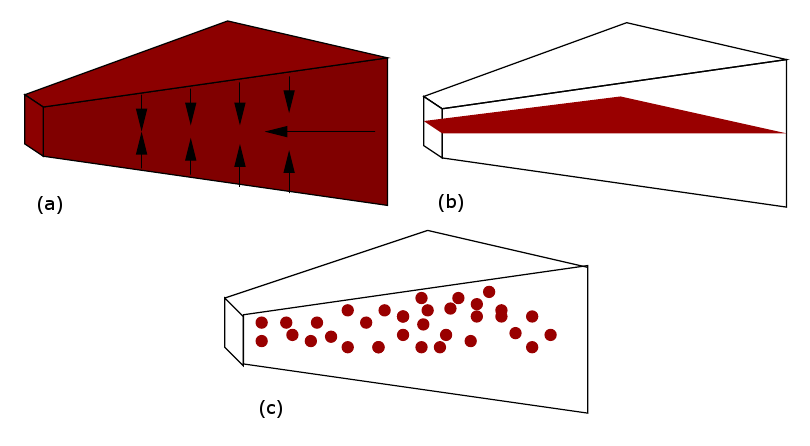
\includegraphics[width=0.9\textwidth]{figures/sedymentacja.png}
   \caption{Ilustracja mechanizmu Goldreicha-Warda. Połączenie sedymentacji pyłu
      na płaszczyznę dysku oraz jego radialnego dryfu (a) może prowadzić do
      wytworzenia się cienkiej i~masywnej warstwy pyłu (b), która jest
      niestabilna grawitacyjnie. Fragmentacja pod wpływem samograwitacji może
      prowadzić do wytworzenia się planetezymali w~lokalnych zagęszczeniach pyłu
      (c). Obrazek pochodzi z~pracy~\cite{armitage}
   }
   \label{fig:GW}
\end{figure}

\par Aby zrozumieć pewne niedostatki powyższej hipotezy, należy
dokładnie przeanalizować procesy zachodzące podczas ewolucji gazowo-pyłowego
dysku okołogwiazdowego. Syntetyczne zestawienie najbardziej istotnych
mechanizmów zostało przedstawione w~dalszej części tego rozdziału.

\par W przypadku gazowych olbrzymów powstających w masywnych dyskach
protoplanetarnych, alternatywną teoria zakłada kolaps i~fragmentację
grawitacyjną całego gazowo-pyłowego dysku~\cite{Boss97}. O tym czy zaburzenia
w~gęstości materii w~dysku będą wzrastać nieograniczenie decyduje równowaga
pomiędzy destabilizującym wpływem samograwitacji, a stabilizującymi
właściwościami ciśnienia oraz rotacji.  Wartość graniczna dla stabilności
cienkiego, osiowo symetrycznego dysku została pierwszy raz wyprowadzona przez
Toomre'ego~\cite{T64}, jako:
%
\begin{equation}
   Q = \frac{c_s\kappa}{\pi G \Sigma}\sim 1,
   \label{eq:toomre}
\end{equation}
%
gdzie $c_s$ to prędkość dźwięku, $\kappa$ częstość epicykliczna, $\Sigma$
gęstość powierzchniowa gazu. Kryterium to z~powodzeniem jest stosowane do
globalnych, stratyfikowanych dysków podlegających nieosiowo symetrycznym
zaburzeniom, tzn. symulacje numeryczne wykazują fragmentację takich dysków dla
$Q\sim 1$~\cite{NBAA98}. W ogólnym przypadku niestabilności grawitacyjnej dysku
kryterium stabilności jest zależne od azymutalnej liczby falowej
$m$~\cite{BT87}. Parametr Toomre'go~\mref{eq:toomre} jest wyprowadzony dla
$m=0$. Jak pokazują symulacje numeryczne~\cite{Duris07} efekt ten zachodzi już
dla $Q\lesssim 1.7$, a więc zanim dysk stanie się na tyle chłodny i~masywny, aby
ulec fragmentacji. Fale spiralne wytwarzają dodatkowe momenty sił i fale
uderzeniowe, które odpowiadają za transport masy i~momentu pędu oraz
podgrzewanie gazu~\cite{YC85}, stabilizując dysk. Kryterium~\mref{eq:toomre} nie
uwzględnia również destabilizujących efektów promienistego (bądź konwekcyjnego)
chłodzenia gazu~\cite{BMD06}. Dokładny przebieg niestabilności grawitacyjnej
w~realistycznych modelach dysków okołogwiazdowych jest ciągle
niejasny~\cite{MB11, LC11}. Niemniej jednak symulacje numeryczne sugerują, że w
masywnych dyskach niestabilność grawitacyjna jest w~stanie wytworzyć związane
obłoki materii o masach $\sim 1\div 10\Mjup$~\cite{BHM10, FR11}. Ich dalsza
ewolucja przebiega podobnie jak w~modelu akrecji jąder tj. pył sedymentuje na
centrum grawitacji tworząc skaliste jądro w~skalach czasowych od $10^3$ do
$10^6$ lat~\cite{HB11, GHB12}. Skalując parametry dysku względem typowych
wartości parametrów fizycznych obserwowanych w~dyskach protoplanetarnych,
parametr $Q$ można wyrazić jako:
%
\begin{equation}
   Q \sim 10^2 
   \left(\frac{T}{100\K}\right)^{0.5}
   \left(\frac{\Sigma}{10^3\g\cm^{-3}}\right)^{-1}
   \left(\frac{R}{1\AU}\right)^{-1.5}.
   \label{eq:Qemp}
\end{equation}
%
Z tego względu niestabilność grawitacyjna ma znaczenie tylko dla zewnętrznych
obszarów dysku protoplanetarnego. Co więcej, związane grawitacyjnie obłoki
podlegają silnemu oddziaływaniu pływowemu~\cite{VH12}, które może prowadzić do
ich rozerwania, a także gwałtownej migracji w~kierunku protogwiazdy~\cite{BMP11}.
\par Niestabilność grawitacyjna nie koniecznie wyklucza się z~modelem akrecji na
jądra, ponieważ może zachodzić już w~trakcie początkowych etapów formowania się
 układu protogwiazda -- dysk (pierwsze kilkaset tysięcy lat), w~przeciwieństwie do
 paru milionów lat w~przypadku akrecji na jądra. Niestabilność grawitacyjna
 również łatwiej tłumaczy powstawanie bardzo masywnych planet, które w~wypadku
 wiodącej teorii wymagają czasu porównywalnego z czasem życia dysku
 protoplanetarnego\cite{HBP}.


\begin{figure}[p]
\centering 
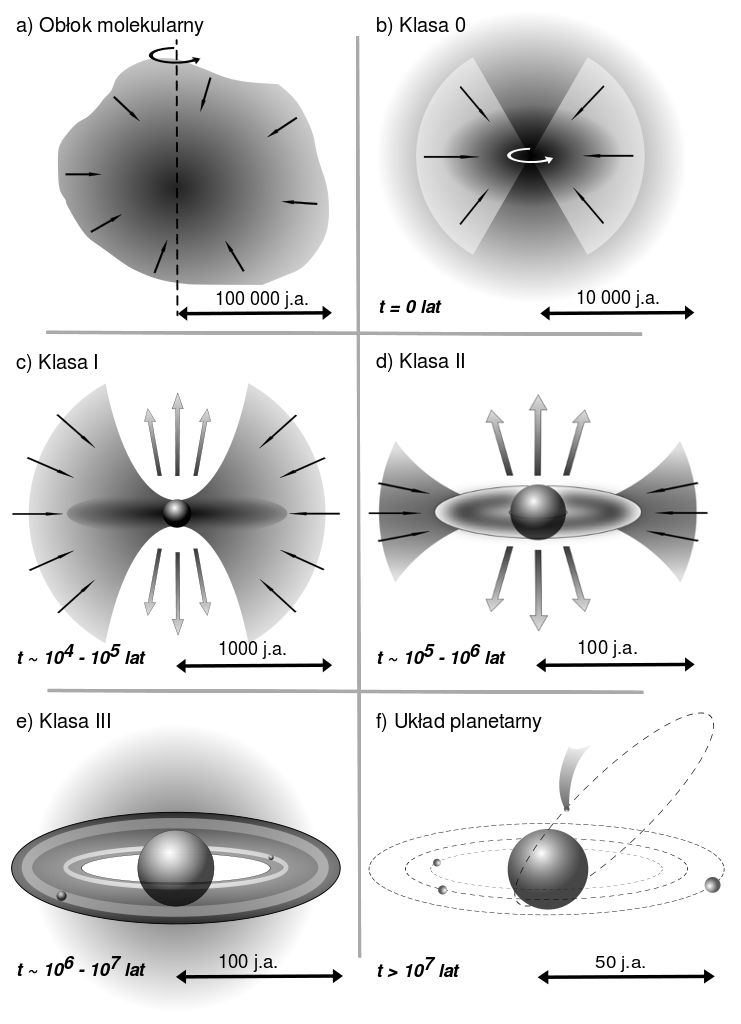
\includegraphics[width=0.9\textwidth]{figures/planetformation.png}
\caption{Ilustracja przedstawia kolejne fazy formowania się mało masywnej gwiazdy
   wraz z~systemem planetarnym: a) kolaps grawitacyjny gęstego obłoku; b)
   oddziaływanie centralnego pola grawitacyjnego oraz siły odśrodkowej powoduje
   opadanie materii i~formowanie się dysku; c) faza FU Orionis: silna akrecja w
   dysku oraz wypływ materii w~okolicach osi obrotu; d) faza T Tauri: zmniejsza
   się tempo akrecji $\sim 10^{-8}\Msun\rok^{-1}$ oraz wypływu materii,
   rozpoczyna się proces formowania planet; e) zanika składowa gazowa, planety
otwierają przerwy w~dysku, następuje również ich migracja; f) cały gaz oraz
mniejsze ciała zostają pochłonięte przez planety lub usunięte z~dysku, układ
planetarny przyjmuje ostateczny kształt. Obrazek zamieszczony dzięki uprzejmości
Joanny Drążkowskiej}

\label{fig:planet}
\end{figure}

\section{Ewolucja dysku protoplanetarnego}
Planety formują się w gazowo--pyłowym dysku, który powstaje podczas kolapsu
obłoku protogwiazdowego. Pewne szczególne mechanizmy oraz globalna dynamika mogą
temu procesowi pomagać, bądź mu przeciwdziałać. Poniższe akapity pokrótce
opisują strukturę dysku protoplanetarnego oraz najważniejsze efekty dynamiczne
związane z~samym gazem, następnie przechodząc do ich wpływu na dynamikę
i~ewolucję pyłu. Pozwoli to wskazać problemy z~jakimi boryka się model ,,akrecji
na jądra'' i~naturalnie przejść do celu tej rozprawy.

\subsection{Struktura dysku protoplanetarnego}
W trackie kolapsu grawitacyjnego obłoku moment pędu jest zachowany. Gdy obłok
rotuje materia nie opada bezpośrednio na obiekt centralny, lecz formuje dysk
w~płaszczyźnie prostopadłej do wektora całkowitego momentu pędu. Aby określić
przybliżone warunki fizyczne w~formującym się dysku możemy posłużyć się
równaniami hydrodynamiki:
%
\begin{gather}
   \partial_t \rho_g + \nabla\cdot\left(\rho_g\mathbf{u}\right) = 0,
   \label{eq:hd1}\\
\partial_t \mathbf{u} + \left(\mathbf{u}\cdot\nabla\right)\mathbf{u} = 
-\nabla\Phi + -\frac{1}{\rho_g} \nabla P, \label{eq:hd2}
\end{gather}
%
gdzie $\rho_g$ jest gęstością gazu, $P$ ciśnieniem, 
związanych z~tarciem, a $\Phi$ potencjałem grawitacyjnym. Jeżeli ponadto
założymy, że dysk jest izotermiczny to
\begin{equation}
   P = n k_{\textrm{B}} T = \frac{\rho k_{\textrm{B}} T}{m_{\textrm{H}}} = \rho
   c_s^2 
\end{equation}
gdzie $c_s$ jest izotermiczną prędkością dźwięku. To implikuje, że gradient
ciśnienia można wyrazić przez:
\begin{equation}
   -\frac{1}{\rho_g}\nabla P = -c_s^2\nabla\ln\rho_g,
\end{equation}
%Przy założeniu stacjonarności równanie~\mref{eq:hd2} 
%
Gdy dysk znajduję się w~równowadze hydrostatycznej w~kierunku $z$ to wertykalne
przyspieszenie grawitacyjne:
%
\begin{equation}
   \partial_z \Phi = g_z = \frac{GM_\star}{r^2}\frac{z}{r} = \Omega^2 z,
\end{equation} 
%
gdzie $M_\star$ to masa gwiazdy macierzystej, $\Omega$ orbitalna częstość
keplerowska, $G$ stała grawitacji Newtona, jest równoważone przez gradient
ciśnienia gazu $\partial_z P / \rho_g$.
Łącząc powyższe założenia otrzymujemy rozkład gęstości gazu:
%
\begin{equation} \label{eq:zeq}
   \rho_g(z) = \frac{\Sigma_G}{H\sqrt{2\pi}} \exp \left[
   \frac{1}{2}\left(\frac{z}{H}\right)^2 \right],
\end{equation}
%
gdzie $\Sigma_g = \int \rho_g(z) dz$ jest gęstością powierzchniową, a
$H=\frac{c_s}{\Omega}$ to charakterystyczna skala grubości dysku.
%
%\par Zakładając w~pierwszym przybliżeniu że dysk jest optycznie gruby, t.j.
%absorbuję całkowicie promieniowanie pochodzące od gwiazdy i~następnie reemituje
%je jako ciało doskonale czarne, można pokazać~\cite{armitage07} że $T \propto
%r^{-3/4}$ i~co za tym idzie $c_s \propto r^{-3/8}$. Dokładniejsze szacunki,
%które lepiej oddają obserwowane dystrucje spektralne energii, można znaleźć w
%pracach~\cite{KenyonHART87, ChaingGold97} {\bf patrz armitage}.
%{\bf Tu raczej trzeba przedstawić tę wersję z~której wynika $T \propto
%r^{-1/2}$}
%
\par W~modelu stacjonarnym warunek równowagi sił radialnych można zapisać
równaniem:
%
\begin{equation}\label{eq:radial_balance}
\frac{u_\phi^2}{r} = \frac{GM_\star}{r^2} +
  \frac{1}{\rho_g}\frac{\textrm{d}P}{\textrm{dr}},
\end{equation}
gdzie $u_\phi^2$ jest prędkością orbitalną gazu.  Kolejne wyrazy
równania~\mref{eq:radial_balance} reprezentują: siłę odśrodkową, siłę
grawitacji, gradient ciśnienia. Wpływ tego ostatniego na globalny rozkład
prędkości jest rzędu $O(H/r)^2$. Dlatego dla cienkich dysków $(H/r \ll 1)$
z~dobrym przybliżeniem można przyjąć, że właściwy moment pędu gazu jest równy
momentowi pędu odpowiadającemu ruchowi keplerowskiemu. Z równania
\mref{eq:radial_balance} wynika zatem, że moment pędu jest monotonicznie rosnącą
funkcją promienia:
%
\begin{equation}\label{eq:angmom}
l = r^2\Omega = \sqrt{GM_\star r}.
\end{equation}
%
Aby materiał z~dysku mógł być akreowany przez gwiazdę macierzystą, w~układzie
musi działać mechanizm powodujący utratę, bądź chociaż redystrybucję momentu
pędu.

\subsection{Transport momentu pędu}
$\ldots$
Obserwacje 
Z obserwacji jasno wynika~\citep{MME04}, że dyski protoplanetarne nie są
obiektami stacjonarnymi. 

Co więcej, obiekty klasy I posiadają wysokie tempa
akrecji $\sim 10^{-5}\Msun\yr^{-1}$. Aby był możliwy radialny przepływ materii
w~kierunku gwiazdy macierzystej, potrzebny jest mechanizm transportu momentu
pędu. W~tym celu trzeba założyć, że ośrodek jest lepki. Zatem należy zastosować
równania Naviera--Stokesa, w których transport momentu pędu jest konsekwencją
siły lepkiej w różniczkowo rotującym dysku (ostatni wyraz po prawej stronie
równania~\mref{eq:ns2}):

\begin{gather}
   \partial_t \rho_g + \nabla\cdot\left(\rho_g\mathbf{u}\right) = 0,
   \label{eq:ns1}\\
\partial_t \mathbf{u} + \left(\mathbf{u}\cdot\nabla\right)\mathbf{u} = 
-\nabla\Phi -\frac{1}{\rho_g} \nabla P + \frac{1}{\rho_g} \nabla \cdot \Pi.
\label{eq:ns2}
\end{gather}
%
Jeżeli dodatkowo założymy, że mamy do czynienia z~płynem newtonowskim, tensor
naprężeń można zredukować do postaci $\Pi = (\rho_g \nu)\nabla\cdot\mathbf{u}$,
gdzie $\nu$ jest lepkością kinematyczną. Całkując układ
równań~\mref{eq:ns1}-\mref{eq:ns2} w~kierunku wertykalnym i~dokonując prostych
przekształceń można otrzymać
\begin{equation}\label{eq:sigma}
   \partial_t \Sigma_g =
   \frac{3}{R}\partial_R\left(\frac{1}{R\Omega}\partial_R\left(R^2\Sigma_g \nu
         \Omega\right)\right).
\end{equation}
Rozwiązaniem stacjonarnym równania~\mref{eq:sigma} jest warunek $\Sigma_g\nu =
\textrm{const}$, co przekłada się na tempo akrecji $\dot{M} = 3\pi\Sigma_g\nu$.
Z powyższego warunku wynika, że lepkość jest własnością ośrodka odpowiedzialną
za akrecję dyskową. Problemem pozostaje wskazanie mechanizmu fizycznego, który
daje przyczynek do lepkości.
\par Podstawowa lepkość, tj. lepkość molekularna $\nu_{\textrm{m}} \sim c_s
\lambda$, gdzie $\lambda = 1 / n\sigma$ to średnia droga swobodna molekuł gazu,
zaś $n$ to koncentracja molekuł gazu, a $\sigma$ ich przekrój czynny, dla
typowych wartości gęstości i~temperatury dysków protoplanetarnych wynosi
$\nu_{\textrm{m}}\sim10^5\cm^2\s^{-1}$~\cite{armitage}. Przekłada się to na
tempo akrecji na poziomie $\dot{M}\sim 10^{-17}\Msun\rok^{-1}$. 
Charakterystyczna skala czasowa takiego procesu $\tau \simeq R^2 /
\nu_{\textrm{m}}$ wynosiłaby $10^{13}\yr$. Z tego względu lepkość molekularną można
całkowicie zaniedbać w~dalszych rozważaniach.
\par W~słynnej pracy Shakura i~Sunyaev~\citep{SS73} zaproponowali, że turbulencja
w dysku może dawać znaczący przyczynek do lepkości, znacząco przewyższający
lepkość molekularną. Dla izotropowej turbulencji, maksymalna skala wirów w~dysku
powinna być proporcjonalna do charakterystycznej skali grubości dysku $H$, zaś
maksymalna prędkość ruchu turbulentnych nie powinna przekraczać prędkości
dźwięku, ponieważ fale uderzeniowe bardzo szybko dyssypują energię kinetyczną.
Shakura i~Sunyaev zaproponowali parametryzację lepkości turbulentnej:

\begin{equation}\label{eq:alpha}
\nu = \alpha c_s H,
\end{equation}
%
gdzie $\alpha$ jest bezwymiarowym parametrem określającym wydajność
turbulencji w~transporcie momentu pędu. Aby wyjaśnić obserwowane tempo akrecji
dla gwiazd \emph{T Tauri}, parametr $\alpha$ powinien być rzędu $10^{-2}$.
Problemem pozostaje wyjaśnienie mechanizmu powstawania turbulencji w~dysku. Z
kryterium Rayleigha~\cite{C61}:
%
\begin{equation}
   \frac{\mathrm{d}}{\mathrm{d}r} j =
   \frac{\mathrm{d}}{\mathrm{d}r}\left(r^2\Omega\right) > 0,
\end{equation}
%
wynika, że hydrodynamiczny dysk keplerowski jest liniowo stabilny. Sytuacja
diametralnie się zmienia jeżeli uwzględnimy obecność w~układzie 
słabego pola magnetycznego. Balbus i~Hawley~\citep{BH91} pokazali, że przepływ
magnetohydrodynamiczny jest stabilny liniowo wtedy i~tylko wtedy, gdy:
%
\begin{equation}\label{eq:mri}
   \frac{\mathrm{d}}{\mathrm{d}r}\left(\Omega^2\right) > 0.
\end{equation}
%
Warunek \mref{eq:mri} \emph{nie jest} spełniony dla dysków keplerowskich. W
rezultacie nawet szczątkowe pole magnetyczne, jest w~stanie wzmocnić wykładniczo
zaburzenia prędkości oraz pola magnetycznego w~gazie w~czasie kilku okresów
orbitalnych, powodując silną
turbulencję. Proces ten określany jest mianem niestabilności magnetorotacyjnej
(MRI). Co więcej, zarówno symulacje lokalne~\cite{DSP10}, jak
i globalne~\cite{FD11} szacują parametr lepkości $\alpha$ dla dysku, w którym
turbulencja została wzbudzona przez MRI na $\alpha\sim 10^{-2}$.
\par Należy zauważyć, że niestabilność magnetorotacyjna wymaga choćby
szczątkowej jonizacji gazu. 

$\ldots$
Jeżeli założymy że źródłem jonizacji jest wysoko energetyczne
promieniowanie pochodzące od gwiazdy macierzystej i~weźmiemy pod uwagę strukturę
pionową dysku~\mref{eq:zeq}, to dojdziemy do wniosku, iż od pewnej wysokości
$h_i$ materia w dysku jest efektywnie osłaniana przez warstwy gazu o $h > h_i$, gdzie
$h_i$ jest wysokością podstawy

zjonizowanego gazu. 
Obszar $h < h_i$ jest zatem \emph{martwą strefą}
w której niestabilność magnetorotacyjna nie występuje~\cite{DFT10} i nie może
być zatem źródłem turbulencji. 

\begin{figure}
   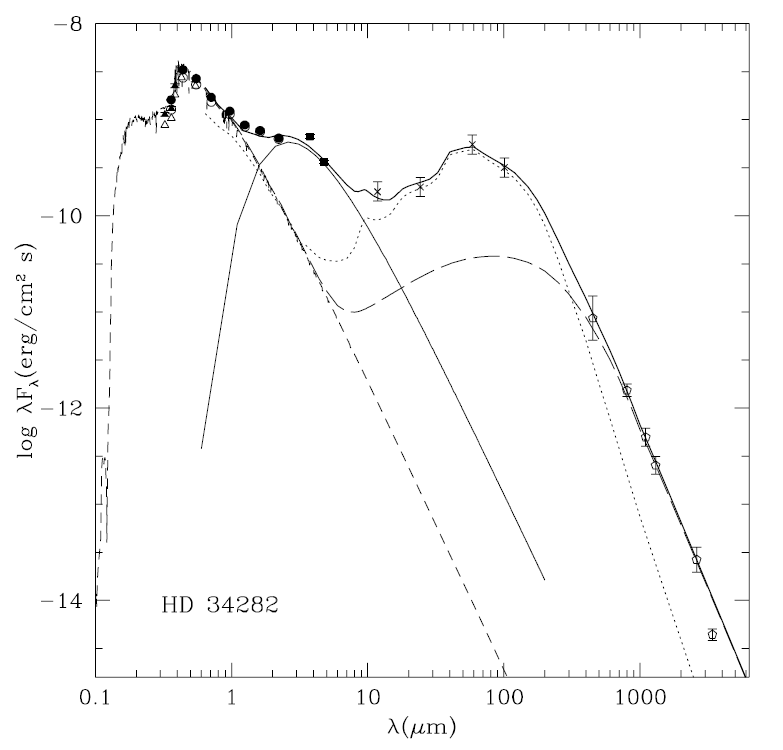
\includegraphics[width=0.9\textwidth]{figures/chap1_sed.png}
   \caption{Rozkład widma energii dla gwiazdy HD 34282~\cite{MME4}. Symbole oznaczają
      obserwacje różnymi metodami dla odpowiednich długości fali. Do obserwacji
      dopasowano następujące modele: linia przerywana model widma gwiazdowego
      dla obiektu typu A3V $(T\sim 8600\K)$, cienka ciągła
      linia model ciała doskonale czarnego dla $T=1400\K$,
      linia kropkowana reprezentuje model dysku o nachyleniu $i=56^o$, tempie
      akrecji $\dot{M} = 8.2\times10^{-9}\thinspace\Msun\yr^{-1}$
      rozciągającym się od $0.31\AU$ do $705\AU$.
   Obrazek pochodzi z~pracy~\cite{MME04}}
   \label{fig:sed}
\end{figure}

\subsection{Oddziaływanie pomiędzy gazem, a pyłem}
Oddziaływanie pomiędzy pyłem a gazem odbywa się poprzez tarcie aerodynamiczne.
Charakterystyczną skalę czasową tego procesu można wyrazić jako~\cite{W73}:
%
\begin{equation}
   \tau_f = \frac{mv_\textrm{pg}}{F_\textrm{D}},
\end{equation}
%
gdzie $m$ i~$v_{\textrm{pg}}\equiv|\mathbf{u} - \mathbf{v}|$ to odpowiednio masa
i prędkość cząstek pyłu względem gazu, zaś $F_\textrm{D}$ to siła tarcia.
$\tau_f$ można interpretować jako czas potrzebny do wytracenia pędu cząstki pyłu
i zrównania jej prędkości z~gazem. Siła $F_\textrm{D}$ jest definiowana w~różny
sposób, w~zależności od rozmiaru ziaren pyłu. Dla cząstek pyłu o promieniu $a < 9
\lambda / 4$ siła tarcia wyraża się prawem Epsteina~\cite{W77}:
%
\begin{equation}
   F_\textrm{D} = \frac{4}{3}\pi a^2 \rho_\bullet \rho_G c_s v_\textrm{pg}, 
\end{equation}
%
gdzie $\rho_\bullet = 1.6\g\cm^{-3}$ jest gęstością materiału, z~którego
zbudowany jest pył. Dla ziaren pyłu o rozmiarach porównywalnych z~drogą swobodną
molekuł gazu, siła tarcia wyraża się poprzez prawo Stokesa~\cite{W77}:
\begin{equation}
  F_\textrm{D} = C_\textrm{D} \pi a^2 \rho \frac{v^2}{2},
\end{equation}
gdzie $v$ to prędkość gazu, zaś współczynnik $C_\textrm{D}$ jest zależny od
liczby Reynoldsa~\cite{W77}:
\begin{equation}
   \textrm{Re} = 2 a \rho \frac{v}{\eta}.
   \label{eq:Re}
\end{equation}
Parametr $\eta$ w równaniu \mref{eq:Re} jest lepkością gazu.
W~niniejszej pracy skupiono się
na obszarach dysków rozciągających się od relatywnie dużych promieni, tj.
$>2\AU$.  Biorąc pod uwagę, iż średnią drogę swobodną możemy wyrazić przez
$\lambda_g = 4.2\times 10^4\textrm{ cm} (10^{-14}\textrm{ g cm}^{-3}/\rho_g)
\approx (R/1 \textrm{AU})^{2.75}\cm$~\citep{W77,BT09}, gdzie $R$ jest odległością
radialną od centrum dysku, prawo Epsteina ma zastosowanie dla dominującej części
domeny obliczeniowej nawet dla największych symulowanych przez nas ziaren pyłu.
Skalę czasową tarcia można wyrazić wzorem:
%
\begin{equation} 
   \tau_f = \frac{\rho_\bullet a} {\rho_g \sqrt{c_s^2 +
      |\mathbf{u} - \mathbf{w}|^2 }} \label{eq:tauf} 
\end{equation}
%
Powodem różnicy prędkości pomiędzy pyłem a gazem może być wiele
procesów, przede wszystkim turbulencja obecna w~gazie, ale także radialny dryf
pyłu (o którym będzie mowa w~dalszej części tego rozdziału) oraz ruchy
Browna. Te ostatnie bardzo silnie zależą od rozmiaru cząstek, tj.
makroskopowe cząstki pyłu praktycznie nie odczuwają ich wpływu, nie są zaś
zależne od gęstości gazu. Ruchy Browna są niezwykle istotne dla rozpoczęcia
procesów koagulacji pyłu w~początkowej fazie formacji
protoplanet~\citep{DD05}, ponieważ skutkują dość znacznym prędkościom względnym
dla najmniejszych ziaren pyłu, które są najsilniej związane z~gazem. Turbulencja
i radialny dryf natomiast tym silniej wpływają na dynamikę, im większa jest
gęstość gazu. Ich znaczenie jest większe dla cząstek o rozmiarach pośrednich, które
są słabiej sprzężone z chaotycznymi ruchami gazu.

\subsection{Radialny dryf pyłu}
Jedno z przybliżeń stosowanych w opisie dysków gazowo-pyłowych opiera się na
założeniu, że pył w~dysku protoplanetarnym można traktować jako bezciśnieniowy płyn. 
Jako że gęstość materii w~dysku zgodnie z założeniami jest malejącą funkcją
promienia, to dla izotermicznego gazu gradient ciśnienia jest ujemny dla całej
rozciągłości dysku. W~rezultacie radialna składowa siły grawitacyjnej dla gazu
jest pomniejszona o gradient ciśnienia. Równanie równowagi sił radialnych:
%
\begin{equation}
   R\Omega_g^2 = \partial_R P / \rho_G + R\Omega_K^2
\end{equation}
%
implikuje, że prędkość orbitalna dla gazu jest nieznacznie mniejsza niż prędkość
keplerowska. Niedobór prędkości rotacji gazu $\delta v = \eta v_\textrm{K}$
względem prędkości orbitalnej opisanej prawem Keplera można określić się jako
bezwymiarowym parametrem~\cite{N86} wyrażonym jako:
%
\begin{equation}
   \label{eq:eta}
   \eta = \frac{\partial_R P}{2\rho_\textrm{G} R \Omega^2} = \frac{1}{2}
   \frac{c_s^2}{v_\textrm{K}^2} \partial_{\ln r} \ln \rho_{\textrm{G}} \approx
   \frac{c_s^2}{v_\textrm{K}^2}.
\end{equation}
%
Dla typowych wartość parametrów, na promieniu $1\AU$, przy $v_\textrm{K}\approx
30\km\s^{-1}$ i~$\eta \approx 10^{-3}$ różnica w~prędkości orbitalnej między
gazem a pyłem wynosi $\Delta v \approx 33\m\s^{-1}$.  W~rezultacie cząstki pyłu
odczuwają permanentny ,,wiatr w~oczy'' skierowany przeciwnie do kierunku ruchu
orbitalnego i~na skutek tarcia trąca swój moment pędu. Efektywność tego procesu
silnie zależy od rozmiaru ziaren pyłu. Drobne cząstki są silnie związane z~gazem
i przez to poruszają się z prędkością bliską prędkości gazu. W rezultacie efekt
oporu aerodynamicznego jest zaniedbywalny. Podobnie dla dużych i~masywnych
obiektów ze względu na ich bezwładność. Najsilniejsza utrata momentu pędu
następuje dla ziaren pyłu spełniających relację $\Omega \tau_f \sim 1$, co
odpowiada cząstkom pyłu o rozmiarach $1\m$ na orbicie o promieniu $1\AU$, bądź
$10\cm$ w~zewnętrznych obszarach dysku.

\begin{figure}
   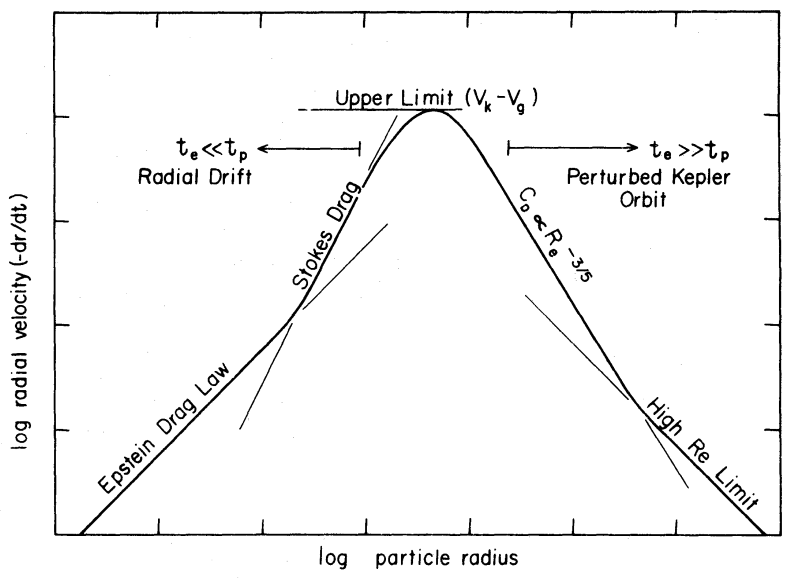
\includegraphics[width=0.9\textwidth]{figures/chap1_drift.png}
   \caption{Schematyczny rysunek zależności pomiędzy rozmiarem ziaren pyłu, a
   maksymalną prędkością radialnego dryfu. Obrazek pochodzi z
   pracy~\cite{W77}}
   \label{fig:chap1_drift}
\end{figure}

Ziarna te są w~stanie osiągać prędkości radialne rzędu
$10^2\div10^3\cm\s^{-1}$~\cite{W77}, co przekłada się na ucieczkę tych cząstek w
kierunku centralnej gwiazdy w~skali czasowej rzędu setek lat!  Kolejną
konsekwencją zależności radialnego dryfu od rozmiaru cząstek jest zróżnicowanie
ich prędkości względem siebie. Cząstki pyłu sklejają się dzięki oddziaływaniom
międzycząsteczkowym, które są szczególnie wydajne w~przypadku małych cząstek
i~dużego ich zagęszczenia. Wraz ze wzrostem cząstek proces zlepiania zachodzi
coraz wolniej.  Siły elektrostatyczne faworyzują małe cząstki, które mają większy stosunek
powierzchni do masy. Przy odpowiednio niskiej prędkości względnej kolizje
prowadzą do tworzenia coraz to większych aglomeratów cząstek~\citep{BW08}, ale
dla dużych różnic w prędkościach najbardziej prawdopodobnym rezultatem zderzenia
jest fragmentacja bądź odbicie~\citep{Z10}. 

\par Nie dość, że czas w którym ziarna pyłu o rozmiarach $0.1 \div 10\m$ mogły
by rosnąć jest niezmiernie krótki, to nie jesteśmy w~stanie wskazać żadnego
mechanizmu powodującego dalszy wzrost rozmiarów pyłu. Problem ten nosi nazwę
\emph{metrowej bariery wzrostu} i~jest najważniejszą niewyjaśnioną kwestię
obecnego paradygmatu formacji planet. 

\par W~ogólności dryf radialny przemieszcza pył w~kierunku maksimum ciśnienia w
gazie. Dla modelu dysku, w którym rozkład gęstości jest opisany funkcją
wykładniczą jest to tożsame z~centrum grawitacji. Należy jednak pamiętać, że
turbulentny ośrodek może wytwarzać lokalne, przejściowe maksima w~ciśnieniu
gazu, dla których gradient będzie dużo większy niż gradient globalny. Z tego
względu obszary o podwyższonym ciśnieniu będą działać jako swoiste pułapki na
pył, przejściowo zwiększając jego gęstość.  Cuzzi, Hogan i~Shariff~\citep{CHS08}
postulują, iż przejściowe zagęszczenia pyłu na skutek ruchów turbulentnych są
wyzwalaczem dla dalszych procesów formowania się planetezymali.
%
\begin{figure}
   \centering
   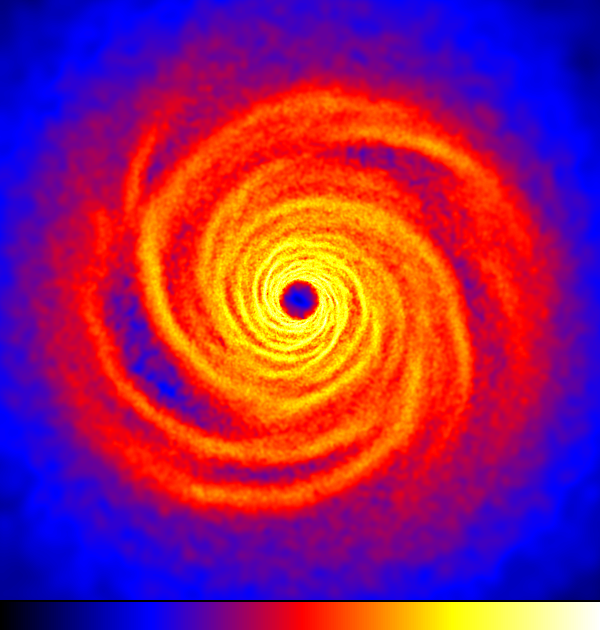
\includegraphics[width=0.46\textwidth]{figures/chap1_gasdisk.png}
   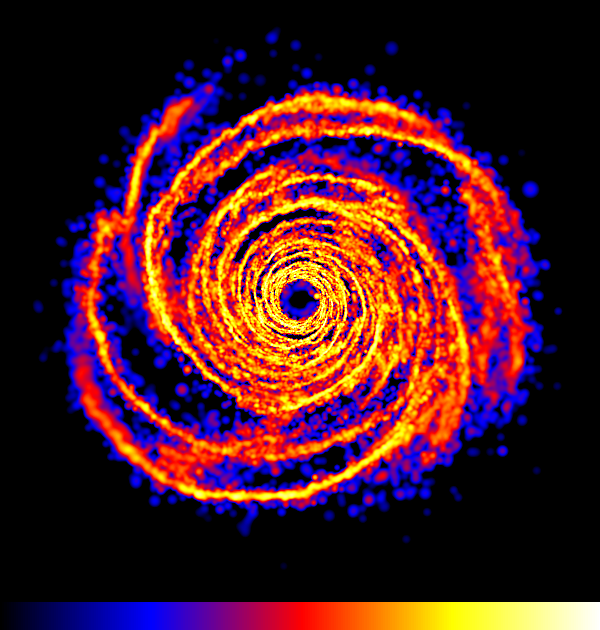
\includegraphics[width=0.46\textwidth]{figures/chap1_dustdisk.png}
   \caption{Symulacja dwuskładnikowego, izotermicznego dysku
      pro\-to\-pla\-ne\-tar\-ne\-go.
      Lewy panel przedstawia rozkład ciśnienia gazu, prawy zaś rozkład gęstości
      gazu. Wy\-raź\-nie widać jak pył jest pułapkowany w~lokalnych maksimach
      ciśnienia. Obrazek za\-po\-ży\-czo\-ny~z pracy~\cite{RLP2006}}
   \label{fig:chap1_trap}
\end{figure}

\subsection{Sedymentacja i~niestabilność Kelvina-Helmholtza (KHI)}
W~dotychczasowych rozważaniach pominęliśmy wpływ pionowej składowej siły
grawitacji pochodzącej od gwiazdy macierzystej na dynamikę ziaren pyłu. O ile
gaz zostaje ściśnięty przez grawitację do momentu osiągnięcia równowagi
hydrostatycznej z gradientem ciśnienia~\mref{eq:zeq}, o tyle opadaniu pyłu nie
przeciwdziała żaden proces fizyczny~\footnote{na chwilę pomińmy fakt, że gaz
jest ośrodkiem turbulentnym i~przez wzajemne sprzężenie wpływa na dynamikę
pyłu}. Sedymentacja mogłaby zatem prowadzić do wytworzenia się cienkiej i~bardzo
gęstej warstwy pyłu, która po przekroczeniu wartości krytycznej rozpadłaby się
pod własnym ciężarem~\citep{GW73}. Zauważmy jednak, że osiadanie pyłu prowadzi
do stopniowego zwiększenia stosunku gęstości pyłu do gazu w~płaszczyźnie dysku.
Ponadto, jak już było wspomniane w~poprzednim podrozdziale, pył porusza się na
wybranej orbicie z~prędkością keplerowską, natomiast gaz pod wpływem radialnego
gradientu ciśnienia z~prędkością podkeplerowską. Duża koncentracja pyłu
w~płaszczyźnie powoduje, że gaz jest efektywniej ,,pchany'' przez pył i~zaczyna
poruszać się szybciej niż warstwy gazu leżące poniżej i~powyżej płaszczyzny
rotacji dysku.  Prowadzi to do wytworzenia się pionowego gradientu prędkości
azymutalnej gazu.  Taka sytuacja powoduje wzbudzenie niestabilności
Kelvina-Helmholtza i~pojawienie się turbulencji w~gazie.  Na skutek wzajemnego
sprzężenia turbulentne ruchy gazu skutkują mieszaniem składnika pyłowego
i~hamowaniem sedymentacji~\cite{JHK06}. Niedawne badania pokazują że tylko
bardzo masywne dyski, o~metaliczności dużo większej niż słoneczna, są nie
wrażliwe na ten proces~\citep{L10}. Podobnie jak w~przypadku niestabilności
magnetorotacyjnej turbulentne ruchy gazu skutkują analogicznymi ruchami pyłu,
jednakże i~w~tym wypadku ustala się pewien stan równowagi dynamicznej między
sedymentacją pyłu, a turbulencją~\cite{JHK06}. 

\subsection{Niestabilność strumieniowa}
Pomimo działania turbulencji wywołanej poprzez szereg opisywanych wcześniej
niestabilności płynowych, w~dysku protoplanetarnym może uformować się warstwa
pyłu o skończonej grubości, dużo mniejszej niż grubość dysku gazowego. Pył ten
jest jednak zbyt rzadki, aby wzbudziła się w~nim niestabilność
grawitacyjna~\cite{JHK06} {\bf jeszcze praca AJ o MRI}.
\par Pomimo tych niesprzyjających warunków istnieje proces który dominuje
ewolucję pyłu w~momencie w~którym stosunek gęstości pyłu do gęstości
gazu zbliża się do jedności. Tym mechanizmem jest {\it niestabilność
strumieniowa} po raz pierwszy przedstawiona w~pracy~\cite{YG05}. Wraz ze
wzrostem gęstości pyłu spowodowanego jego dryfem w~kierunku najbliższego
maksimum ciśnienia gazu, wzrasta wypadkowa siła z~jaką pył oddziałuje na gaz.
Prowadzi to zwiększenia prędkości gazu i~wzrostu ciśnienia na skutek zagarniania
obszarów gazów poruszających się wolniej. Zwiększa to maksimum ciśnienia w~gazie
i przyspiesza dryft pyłu z~otaczających go obszarów. W~przypadku braku działania
dodatkowych sił, gradient ciśnienia skierowany na zewnątrz gęstniejącego obszaru
powodowałby jego szybkie rozmycie, ale w~wypadku rotującego dysku połączenie
ciągłego dryfu pyłu i~siły Coriolisa prowadzi do wytworzenia się równowagi
geostroficznej~\cite{JBL11}. Nasycenie gęstości pyłu następuje w~momencie gdy
masa porcji pyłu jest w~stanie wyrwać się z~lokalnego maksimum gazu.  Nawet
zaniedbując efekt samograwitacji w~trakcie ewolucji niestabilności strumieniowej
lokalna gęstość pyłu może zwiększyć się tysiąckrotnie~\cite{JY07}, co może
prowadzić do wytworzenia się grawitacyjnie związanych obiektów~\cite{J07}.
Niedawne badania niestabilności strumieniowej skupiały się na różnych aspektach
fizycznych które mają wpływ na jej rozwój t.j.: uwzględnienie szerokiego
spektrum rozmiaru cząstek pyłu~\cite{BS10a}, wpływ globalnego gradientu
ciśnienia w~dysku okołogwiazdowym~\cite{BS10b}, stratyfikacja dysku~\cite{T12}.
Niemniej jednak wszystkie publikacje były ograniczone do lokalnego
przybliżenia dysku.

\section{Cel i plan pracy}
Głównym celem pracy jest zbadanie niestabilności strumieniowej w~
realistycznym przybliżeniu radialnie rozciągłego dysku.

Celem badań jest oszacowanie i~opis wpływu niestabilności strumieniowej na
proces generowania lokalnego wzrostu stosunku gęstości pyłu do gazu w~globalnym
dysku pyłowo-gazowym. Pył jako ważny składnik dysku okołogwiazdowego można
opisywać w~przybliżeniu płynowym (funkcja już zaimplementowana w~kodzie PIERNIK
patrz (Hanasz, et al. 2009b) lub w~przybliżeniu punktów materialnych. Obecnie w
literaturze naukowej dominuje druga  metoda, ważne jest więc jakościowa
i~ilościowa weryfikacja własności niestabilności strumieniowej w przybliżeniu
płynowym.


%%%%%%%%%%%%%%%%%%%%%%%%%%%%%%%%%%%%%%%%%%%%%%%%%%%%%%%%%%%%%%%%%%%%%%%%%%%%%%%%
% vim: tw=80 ts=3: 

%\begin{savequote}[75mm]
%   $\ldots$\qauthor{$\ldots$}
%\end{savequote}

\chapter{Liniowa analiza stabilności}
\label{sec:lsa}
W~tym rozdziale przedstawiono poszczególne kroki liniowej analizy stabilności
dla niestabilności strumieniowej w oparciu o pracę~\citep{YG05}.
Analiza stabilności opiera się na trzech elementach:
\begin{enumerate}
   \item znalezieniu stanu równowagi dla zadanego układu równań,
   \item zadaniu zaburzeń o małej amplitudzie,
   \item znalezieniu modów własnych problemu liniowego, ich częstości oraz
      liniowego tempa wzrostu. 
\end{enumerate}
Niestety dla układu równań hydrodynamiki dwóch sprzężonych płynów w~rozciągłym
dysku keplerowskim nie istnieje warunek równowagowy. Spowodowane jest to
migracja pyłu na centrum grawitacji na skutek utraty momentu pędu przez tarcie
aerodynamiczne. Naturalną konsekwencją migracji są znaczne zmiany w~radialnym
profilu rozkładu gęstości pyłu. Należy jednak zauważyć, że charakterystyczna
skala czasowa migracji jest rzędu setek bądź więcej lat, przy założeniu iż mamy
do czynienia z~aglomeratami pyłu o rozmiarach metrowych. Z~tego względu możemy
założyć że zmiany w~profilu gęstości są procesem powolnym w~stosunku do typowego
tempa wzrostu niestabilności strumieniowej, co zostanie wykazane w~dalszej
części pracy.

Kolejnym utrudnieniem jest radialna rozciągłość rozważanego dysku
okołogwiazdowego, która implikuje zależność stanu niezaburzonego od
promienia dysku. W~tym wypadku najogólniejszym podejściem byłaby
globalna analiza stabilności po przez rozwiązanie dwupunktowego problem
brzegowego (np.~\cite{PHM04, KH06}), jednakże takie podejście jest dużo bardziej
skomplikowane. Przedstawianą tu lokalną analizę należy zatem traktować jako
pierwsze przybliżenie pełnej liniowej analizy niestabilności strumieniowej.
Niestabilne mody uzyskane w~ramach liniowej analizy posłużą nam jako punkt
odniesienia dla modów uzyskiwanych w~globalnym eksperymencie numerycznym.

Najbardziej wygodnym układem do lokalnego opisu niestabilności strumieniowej
jest tzw. kostka ścinana~\footnote{ang. shearing box}~\citep{HGB95}, czyli
kartezjański układ współrzędnych, którego początek współporusza się z~płynem na
wybranej orbicie $R_0$ z~częstością keplerowską $\Omega_0 \equiv
\Omega\left(R_0\right)$. Zwyczajowo przyjmuje się, że oś $x$ jest skierowana
radialnie na zewnątrz, oś $y$ jest w~kierunku azymutalnym, zaś $z$ jest osią
wertykalną. Zgodnie z~pracą~\cite*{YJ07} układ równań ciągłości oraz ruchu dla
obu składników można wyrazić poprzez:
%
\begin{align}
\partial_t \rho_g &+ \mathbf{u}\cdot\nabla\rho_g - \frac{3}{2}\Omega x\partial_y\rho_g 
 = -\rho_g\nabla\cdot\mathbf{u},\label{eqc1}\\
\partial_t \rho_d &+ \mathbf{w}\cdot\nabla\rho_d - \frac{3}{2}\Omega x\partial_y\rho_d 
 = -\rho_d\nabla\cdot\mathbf{w},\label{eqc2}\\
\partial_t \mathbf{u} &+ \left(\mathbf{u}\cdot\nabla\right)\mathbf{u} 
 - \frac{3}{2}\Omega x\partial_y\mathbf{u} 
 = 2\Omega u_y \hat{\mathbf{x}} -\frac{1}{2}\Omega u_x \hat{\mathbf{y}} \notag\\
 &- \frac{\epsilon}{\tau_f}(\mathbf{u}-\mathbf{w}) -c_s^2\nabla\ln\rho_g 
 +2\eta\Omega^2 R \hat{\mathbf{x}},\label{eqm1}\\
\partial_t \mathbf{w} &+ \left(\mathbf{w}\cdot\nabla\right)\mathbf{w} 
 - \frac{3}{2}\Omega x\partial_y\mathbf{w}
 = 2\Omega w_y \hat{\mathbf{x}} -\frac{1}{2}\Omega w_x \hat{\mathbf{y}} \notag\\
 &- \frac{1}{\tau_f}(\mathbf{w}-\mathbf{u}), \label{eqm2}
\end{align}
%
gdzie wyrazy takie jak $(3/2)\Omega x$ po lewej stronie równań, pojawiają się na
skutek transformacji wszystkich prędkości względem liniowego, ścinanego przepływu
$\mathbf{v}_0 = -(3/2)\Omega x \hat{\mathbf{y}}$ w~rotującym układzie
współrzędnych. Warto nadmienić, że wyraz $-(1/2)\Omega \{u,w\}_x
\hat{\mathbf{y}}$ po prawej stronie równań ruchu \mref{eqm1}-\mref{eqm2} jest
sumą dwóch składników: $(-2\Omega \{u,w\}_x + (3/2)\Omega \{u,w\}_x)
\hat{\mathbf{y}}$ z~których pierwszy jest składową siły Coriolisa, a drugi
wynika z~odjęcia wspomnianego wcześniej przepływu średniego. Główną różnicą
pomiędzy równaniami \mref{eqm1} oraz \mref{eqm2} jest brak wyrazu ciśnieniowego
dla składnika pyłowego. YG05 zauważyli, że można w~spójny sposób uwzględnić
globalny, radialny gradient ciśnienia gazu w~ramach kostki ścinanej, poprzez
dodanie liniowego wyrazu, który jest sparametryzowany wielkością określającą
bezwymiarową miarę rotacji podkeplerowskiej:

\begin{equation}
\eta \equiv - \frac{\partial_R P}{2\rho_g\Omega^2 R} \sim \frac{c_s^2}{v_K^2}.
\end{equation}

Układ równań \mref{eqc1}-\mref{eqm2} posiada znane rozwiązanie równowagowe~\citep{N86}

\begin{align}
\bar{\mathbf{w}} &= \left[ 
 -2\tau_s\xi, \frac{\tau_s^2\xi - 1}{1+\epsilon},
 0
\right]\eta v_K, \label{eq:w0}\\
\bar{\mathbf{u}} &= \left[ 
 2\epsilon\tau_s\xi, -\frac{1 + \epsilon\tau_s^2\xi}{1+\epsilon},
 0
\right]\eta v_K, \label{eq:u0}
\end{align}
%
gdzie $\tau_s = \Omega \tau_f$ to bezwymiarowy \emph{czas
zatrzymania}~\footnote{ang. dimensionless stopping time} i~$\xi =
((1+\epsilon)^2 + \tau_s^2)^{-1}$.  Linearyzacja równań \mref{eqc1}-\mref{eqm2},
polega na rozbiciu zmiennych na część stałą $\bar{\mathbf{q}}$ oraz zaburzenie
$\mathbf{q}^\prime$. W~rezultacie $\mathbf{q} =
\bar{\mathbf{q}} + \mathbf{q}^\prime$, gdzie $\mathbf{q}=[\rho_d, w_x, w_y, w_z,
\rho_g, u_x, u_y, u_z]$. Zakładamy równocześnie, że zaburzenie przyjmuje postać
osiowo-symetrycznej fali płaskiej:

\begin{equation}
   \label{eq:planar}
   \mathbf{q}^\prime(x,z,t) = \tilde{\mathbf{q}}
 \exp\left[i(k_x x + k_z z~-\omega t)\right]
\end{equation}

Po~podstawieniu liniowego zaburzenia układ równań przyjmuje następującą postać

\begin{align}
-i(\omega- k_x\bar{w}_x)\tilde{\rho}_d &= 
 - i~\bar{\rho}_d(k_x\tilde{w}_x + k_z\tilde{w}_z), \label{lin1}\\
-i(\omega- k_x\bar{u}_x)\tilde{\rho}_g &= 
 - i~\bar{\rho}_g(k_x\tilde{u}_x + k_z\tilde{u}_z), \label{lin2}\\
-i(\omega- k_x\bar{u}_x)\tilde{\mathbf{u}} &= 
 2\Omega \tilde{u}_y\hat{\mathbf{x}} - \frac{1}{2}\Omega \tilde{u}_x
 \hat{\mathbf{y}}
 -\frac{\epsilon}{\tau_f}(\tilde{\mathbf{u}} - \tilde{\mathbf{w}}) \notag\\
  -\frac{\tilde{\rho}_d}{\bar{\rho}_g\tau_f}
  (\bar{\mathbf{u}} &- \bar{\mathbf{w}})
  - \frac{c_s^2}{\bar{\rho}_g}ik_x\tilde{\rho}_g\hat{\mathbf{x}} -
  - \frac{c_s^2}{\bar{\rho}_g}ik_z\tilde{\rho}_g\hat{\mathbf{z}}, \label{lin3}\\
-i(\omega- k_x\bar{w}_x)\tilde{\mathbf{w}} &= 
 2\Omega \tilde{w}_y\hat{\mathbf{x}} - \frac{1}{2}\Omega \tilde{w}_x
 \hat{\mathbf{y}} 
 - \frac{1}{\tau_f} (\tilde{\mathbf{w}} - \tilde{\mathbf{u}}), \label{lin4}
\end{align}
%
gdzie $\epsilon = \bar{\rho}_d/\bar{\rho}_g$. Układ równań
\mref{lin1}-\mref{lin4} można zapisać jako

\begin{equation}
 \eurom{A}(k_x,k_z,\omega)\tilde{\mathbf{q}} = 0,
 \label{eq:linset}
\end{equation}
gdzie 
\begin{equation}
 A =
 \setlength\arraycolsep{2pt}
 \begin{bmatrix}
    -i\tilde{\omega}_d & i~k_x \bar{\rho}_d & 0 & i~k_z \bar{\rho}_d & 0 & 0 & 0 & 0 \\
    0 & \frac{1}{\tau_f} -i \tilde{\omega}_d & -2\Omega & 0 & 0 & \frac{1}{\tau_f} & 0 & 0 \\
    0 & \frac{1}{2}\Omega & \frac{1}{\tau_f} -i \tilde{\omega}_d & 0 & 0 & 0 & \frac{1}{\tau_f} & 0 \\
    0 & 0 & 0 & \frac{1}{\tau_f} -i \tilde{\omega}_d & 0 & 0 & 0 & \frac{1}{\tau_f} \\
    0 & 0 & 0 & 0 & -i\tilde{\omega}_g & i~k_x \bar{\rho}_g & 0 & i~k_z \bar{\rho}_g \\
    \frac{\bar{u}_x - \bar{w}_x}{\tau_f \bar{\rho}_g} & -\frac{\epsilon}{\tau_f} & 0 & 0 &
    \frac{c_s^2}{\bar{\rho}_g i~k_x} & \frac{\epsilon}{\tau_f}-i\tilde{\omega}_g &
    -2\Omega & 0\\
    \frac{\bar{u}_y - \bar{w}_y}{\tau_f \bar{\rho}_g} & 0 & -\frac{\epsilon}{\tau_f} & 0 & 0 &
    \frac{1}{2}\Omega & \frac{\epsilon}{\tau_f} -i \tilde{\omega}_g & 0 \\
    0 & 0 & 0 & -\frac{\epsilon}{\tau_f} & \frac{c_s^2}{\bar{\rho}_g i~k_z} & 0 & 0 &
    \frac{\epsilon}{\tau_f} -i \tilde{\omega}_g
 \end{bmatrix}
%
\end{equation}
zaś $\tilde{\omega}_d = \omega - k_x \bar{w}_x$ i~$\tilde{\omega}_g = \omega -
k_x \bar{u}_x$.
%
Nietrywialne rozwiązania układu liniowego \mref{eq:linset} istnieją wtedy i~tylko
wtedy gdy równanie dyspersyjne 
\begin{equation}
 \det|\eurom{A}(k_x,k_z,\omega)|=0.
 \label{eq:disprel}
\end{equation}
%
Dla zadanych wartości $(k_x, k_x)$ relację \mref{eq:disprel} można rozwiązać ze
względu na $\omega$ i~dzięki temu otrzymać związki pomiędzy amplitudami
składowych wektora $\tilde{\mathbf{q}}$.
Tempo wzrostu niestabilności definiujemy jako urojoną część zespolonej
częstotliwości $s=\Im(\omega)$.
%
Analiza  liniowej fazy wzrostu niestabilności strumieniowej wzbudzanej w
symulacjach została przedstawiona w podrozdziale~\ref{sec:simulation_analysis},
gdzie porównano tempo wzrostu najszybciej roznących modow w eksperymentach
numerycznych do tempa wzrostu obliczonego jako rozwiązanie związku
dyspersyjnego~\mref{eq:disprel}. Podobnie liczby falowe  najszybciej rosnących
modów niestabilności w eksperymentach numerycznych zostaną porównane z
przewidywaniami analitycznymi.

%%%%%%%%%%%%%%%%%%%%%%%%%%%%%%%%%%%%%%%%%%%%%%%%%%%%%%%%%%%%%%%%%%%%%%%%%%%%%%%%
% vim: tw=80 ts=3: 

\begin{savequote}[75mm]
Strike hot iron and call forth sparks; strike a man and call forth fury; to shape man or metal to thy will, thou must
strike with force.
\qauthor{Collected Sermons of Carras, Thief by Looking Glass Studios}
\end{savequote}

\chapter{Eksperyment numeryczny}
\section{Metodyka}
\label{sec:metodyka}
Badania zaprezentowane w niniejszej pracy opierają się na szeregu eksperymentach
numerycznych wykonanych z pomocą autorskiego kodu płynowego PIERNIK tworzonego
od 2006 roku w Centrum Astronomii UMK.  Algorytmy numeryczne kodu PIERNIK
opierają się na zachowawczym schemacie płynowym typu ,,Relaxing
TVD''~\cite{jin-xin-95} w połączeniu z~dzielonym, kierunkowym całkowaniem
przestrzennym i~czasowym przy użyciu algorytmu\linebreak Runge-Kutta drugiego
rzędu~\cite{2003PASP..115..303T,2003ApJS..149..447P}. Konstrukcja kodu umożliwia
modelowanie wieloskładnikowego ośrodka np. płynu neutralnego i~płynu
bezciśnieniowego (pył) z uwzględnieniem oddziaływań
międzypłynowych~\cite{piernik1,piernik2}. PIERNIK wyposażony jest w
wielosiatkowy algorytm przeznaczony do wyznaczania przybliżonych rozwiązań
równań różniczkowych typu parabolicznego i eliptycznego, a w szczególności
solwer multigridowy pozwalający efektywnie rozwiązywać paraboliczne
i~eli\-pty\-czne równania różniczkowe, w~tym równanie Poissona opisujące
samograwitację pyłu~\citep{HG00}. Ponadto w kodzie PIERNIK zaimplementowano
solwer multipolowy pozwalający na szybkie określenie warunków brzegowych dla
potencjału grawitacyjnego~\citep{J77} oraz możliwość prowadzenia obliczeń na
siatkach w cylindrycznym układzie współrzędnych przy zachowaniu moment pędu do
poziomu numerycznej precyzji~\cite{M07,SO10}. Kod PIERNIK posiada również
implementację algorytmu szybkiego transportu eulerowskiego~\footnote{ang.
\emph{Fast Advection in Rotating Gaseous Objects -- FARGO}}~\citep{M00} w~ujęciu
wielopłynowym.
\par 
Ponadto PIERNIK korzysta z~algorytmu typu \emph{Constraint
Transport}~\cite{EH88} zapewniającego spełnienie warunku bezźródłowości pola
magnetycznego, a także możliwość wykonywania symulacji przy użyciu siatek
adaptywnych~\footnote{ang.  \emph{Adaptive Mesh Refinement -- AMR}}. Kod został
zrównoleglony przy użyciu protokołu MPI i wykazuje dobrą silną jak i bardzo
dobrą słabą skalowalność w zakresie do $10^4$ rdzeni obliczeniowych.
%
\par Obliczenia opisywane w~tej pracy zostały przeprowadzone z~wykorzystaniem:

\begin{itemize}
   \item infrastruktury PL-Grid, w~szczególności klastrów
      komputerowych Galera+ (Trójmiejska Akademicka Sieć Komputerowa), Hydra
      (Interdyscyplinarne Centrum Modelowania Matematycznego i Komputerowego),
      Zeus (Akademickie Centrum Komputerowe CYFRONET), Inula (Poznańskie Centrum
      Superkomputerowo Sieciowe) w~ramach grantu \emph{plggpiernik},

   \item klastrów PRACE, w~szczególności klastrów komputerowych
      Cartesius (SurfSara), Fionn (Irish Centre for High-end Computing) w~ramach grantu \emph{PIERNIK-SI} w
      projekcie Distributed European Computing Initiative (DECI-11).
\end{itemize}
Sumaryczne zużycie wyniosło kilka milionów CPUh.


%We conduct numerical simulations with the aid of a
%parallel MHD code PIERNIK using the cylindrical coordinate system. 


\subsection{Podstawowe równania}
W dalszych rozważaniach założymy, że opis dynamiki gazowo-pyłowego dysku
okołogwiazdowego może być oparty na układzie równań opisujących dwa oddziałujące
dynamicznie płyny - gaz w przybliżeniu izotermicznym oraz  pył traktowany jako
płyn bezciśnieniowy. Równania hydrodynamiki przyjmują dla takiego modelu
następującą postać:
%
% CONSERVATIVE FORM
\begin{align}
   \partial_t \rho_g &+ \nabla\cdot\left(\rho_g\mathbf{u}\right) = 0,\label{eq1}\\
   \partial_t \rho_d &+ \nabla\cdot\left(\rho_d\mathbf{w}\right) = 0,\label{eq2}\\
\partial_t \left(\rho_g\mathbf{u}\right) &+
   \nabla\cdot(\mathbf{u}\otimes(\rho_g\mathbf{u})+P) \notag\\
 &= -\rho_g\left(\nabla\Phi +
\frac{\rho_d}{\tau_f\rho_g}(\mathbf{u}-\mathbf{w})\right),\label{eq3}\\
\partial_t \left(\rho_d\mathbf{w}\right) &+
\nabla\cdot(\mathbf{w}\otimes(\rho_d\mathbf{w})) \notag\\
 &= -\rho_d\left(\nabla\Phi + \frac{1}{\tau_f}(\mathbf{w}-\mathbf{u})\right)
\label{eq4}.
\end{align}
% NON-CONSERVATIVE FORM
%\begin{align}
%\partial_t \rho_g &+ \nabla\cdot\left(\rho_g\mathbf{u}\right) = 0,\\
%\partial_t \rho_d &+ \nabla\cdot\left(\rho_d\mathbf{w}\right) = 0,\\
%\partial_t \mathbf{u} &+ \left(\mathbf{u}\cdot\nabla\right)\mathbf{u} = 
% -\nabla\Phi + \frac{\rho_d}{\tau_f\rho_g}(\mathbf{w}-\mathbf{u})
% -c_s^2\nabla\ln\rho_g,\label{eq3} \\
%\partial_t \mathbf{w} &+ \left(\mathbf{w}\cdot\nabla\right)\mathbf{w} = 
% -\nabla\Phi - \frac{1}{\tau_f}(\mathbf{w}-\mathbf{u}),\label{eq4}
%\end{align}

\noindent gdzie $\rho_g$, $\rho_d$ to odpowiednio gęstości gazu i~pyłu,
$\mathbf{u}$, $\mathbf{w}$ ich prędkości, $P$ to ciśnienie gazu, $\tau_f$ jest
skalą czasową tarcia~\footnote{ang. friction time}~\mref{eq:tauf}, a $\Phi$ to
potencjał grawitacyjny.

\par Ze względu na specyfikę zagadnienia badanego w~niniejszej pracy
najwygodniejszym układem współrzędnych jest układ cylindryczny. W~kodzie PIERNIK
równania mechaniki płynów w geometrii cylindrycznej wyrażone są w postaci
zachowującej moment pędu~\cite{M07,SO10}, która wprowadza tylko jeden, dodatkowy
wyraz źródłowy do równań ruchu~\mref{eq3} - \mref{eq4}: odpowiednio
$\left((\rho_g u_\phi + P) / R\right)\mathbf{\hat{R}}$ oraz $(\rho_d w_\phi / R)
\mathbf{\hat{R}}$.
%
\par Przyspieszenie będące skutkiem wzajemnego oddziaływania pyłu i gazu
przyjmuje postać $\rho_d/\tau_f\rho_g(\mathbf{u}-\mathbf{w})$
i~$1/\tau_f(\mathbf{w}-\mathbf{u})$ odpowiednio dla równań \mref{eq3}
i~\mref{eq4} w~zależności od tego jak zostanie potraktowane, może prowadzić do
znacznego skrócenia kroku czasowego. Z tego względu zdecydowano o implementacji
pół niejawnego schematu modyfikującego bezpośrednio prędkości gazu i~pyłu,
opisanego w pracy~\cite{TB09}.

%W~ramach pracy skupiono się na dyskach rozciągających się relatywnie dużych
%promienii tj. 2~AU. Zakładając, za pracą~\cite{CD93}, że przejście do
%reżimu Stokesa zachodzi dla ziaren pyłu o promieniu większym niż
%$a = 9/4\lambda_g$ gdzie $\lambda_g = 4.2\times 10^4\textrm{
%cm} (10^{-14}\textrm{ g cm}^{-3}/\rho_g) \approx (R/1 \textrm{AU})^{2.75}$~cm 
%jest średnią drogą swobodną molekuł gazu~\citep{W77,BT09}, zaś $R$ jest
%odległością radialną od centrum dysku. Przy tych założeniach, reżim Epstein ma
%%zastosowanie dla dominującej części domeny obliczeniowej nawet dla największych
%symulowanych przez nas ziaren pyłu. Skala czasowa tarcia przyjmuję zatem
%następującą postać:
%

\subsection{Podstawowy algorytm płynowy kodu PIERNIK}
Do rozwiązania układu równań \mref{eq1}--\mref{eq4}, jak wspomniano wcześniej
użyta została tzw. \textit{metoda relaksacji TVD}~\cite{jin-xin-95}, która
zapewnia wysoką dokładność rozwiązań równań hydrodynamicznych oraz numeryczną
stabilność, przy stosunkowo niskich nakładach mocy obliczeniowych. Poniżej
przedstawiono krótki \textit{metody relaksacji TVD} na przykładzie równania

\begin{equation}\label{diffeuler}
   \partial_t \mathbf{u} + \partial_{x} \mathbf{F}(\mathbf{u}) = 0.
\end{equation}
wzorując się na pracach Trac \& Pen~\cite*{2003PASP..115..303T}
oraz Pen, et al.~\cite*{2003ApJS..149..447P}, które zostały użyte jako punkt
wyjścia przy tworzeniu \textbf{PIERNIKa}. 

\paragraph{Podział ,,zaburzenia'' na fale biegnące w~prawą i~lewą stronę.} ~\\
%
Zgodnie z pracą Trac\&Pen~\cite{2003PASP..115..303T} układ \mref{diffeuler}
można zastąpić układem postaci:
%
\begin{gather}
   \partial_t \mathbf{u} + \partial_x (c\mathbf{w}) = 0, \label{rel1}\\
   \partial_t \mathbf{w} + \partial_x (c\mathbf{u}) = 0, \label{rel2}
\end{gather}
%
gdzie $c(x,t)$ jest dowolną, dodatnią funkcją większa co do modułu od
największej prędkości falowej układu: 
%
\begin{equation}\label{fs}
   c \ge |v| + c_s,
\end{equation}
nazywaną \emph{prędkością mrożącą}, a $\mathbf{w} = \mathbf{F}(\mathbf{u})/c$. 
Równanie \mref{fs}, zgodnie z~warunkiem CFL zapewniającym stabilność schematu
%
\begin{equation}\label{cfl}
   \frac{c_{\textrm{max}}\Delta t}{\Delta x} \le 1,
\end{equation}
%
nakłada nam silne ograniczenie na krok czasowy.  Układ relaksacyjny zawiera dwa
sprzężone, liniowe równania adwekcji wielkości zachowawczych $\mathbf{u}$ oraz
$\mathbf{w}$. Aby rozwiązać równania \mref{rel1} i~\mref{rel2} należy dokonać
zamiany zmiennych:
%
\begin{gather}
   \mathbf{u}^R = \frac{\mathbf{u} + \mathbf{w}}{2}, \\
   \mathbf{u}^L = \frac{\mathbf{u} - \mathbf{w}}{2}, \\
   \intertext{co pozwala zapisać}
   \partial_t \mathbf{u}^R + \partial_x (c\mathbf{u}^R) = 0,\label{rel3}\\
   \partial_t \mathbf{u}^L + \partial_x (c\mathbf{u}^L) = 0.\label{rel4}
\end{gather}
%
Równania \mref{rel3} i~\mref{rel4} można interpretować jako prawa zachowania
opisujące propagację fal w~pra\-wą i~lewą stronę z~prędkością $c$. Sumując można
je wyrazić jako
%
\begin{equation}
   \partial_t \mathbf{u} + \partial_x \mathbf{F}^R - \partial_x \mathbf{F}^L = 0,\\
\end{equation}
%
gdzie $\mathbf{F}^R=c \mathbf{u}^R$ i~$\mathbf{F}^L=c \mathbf{u}^L$. 
%
\paragraph{Obliczenie strumieni wielkości zachowawczych metodą \emph{,,pod wiatr''}.}~\\
%
W~celu rozwiązania \mref{rel3} i~\mref{rel4} należy policzyć strumienie
wielkości zachowawczych. W~podstawowej wersji \textbf{Piernika--MHD} strumienie
na brzegach komórek są liczone z~dokładnością do drugiego rzędu w~przestrzeni
$\left(\epsilon \sim O\left[(\Delta x)^2\right]\right)$. 
Podwyższenie dokładności schematu następuje poprzez monotoniczną interpolację
strumieni obliczonych w centrach komórek na ściany. Reprezentacja pochodnych za
pomocą różnic skończonych obliczanych metodą \emph{,,pod wiatr''}\footnote{ang.
,,upwind'' method}~\cite{cir}, zapewnia stabilność numeryczną schematu.
Korzystając z definicji strumienia $\mathbf{F}_n^{(1),t}=c \mathbf{u}_n^t$, jako
wielkości określonej na środku komórki, w~zależności od kierunku propagacji fali
strumień na brzegu jest obliczany w~następujący sposób:
%
\begin{equation}
   \mathbf{F}^{(1),t}_{n+1/2} = 
   \begin{cases}
      \mathbf{F}^{(1),t}_{n}  \quad \textrm{jeżeli }c>0,\\
      \mathbf{F}^{(1),t}_{n+1}\quad \textrm{jeżeli }c<0.
   \end{cases}
\end{equation}
%
Następnie liczona jest poprawka strumieni drugiego rzędu, ponownie z
uwzględnieniem kierunku propagacji fali:
%
\begin{align} \label{lab1}
   \begin{cases} 
      \Delta \mathbf{F}^{L,t}_{n+1/2} = \frac{\mathbf{F}^t_{n} - \mathbf{F}^t_{n-1}}{2} \\
      \Delta \mathbf{F}^{R,t}_{n+1/2} = \frac{\mathbf{F}^t_{n+1} - \mathbf{F}^t_{n}}{2}
   \end{cases} \textrm{ dla prędkości }c>0,\\
   \label{lab2}\begin{cases} 
   \Delta \mathbf{F}^{L,t}_{n+1/2} = -\frac{\mathbf{F}^t_{n+1} - \mathbf{F}^t_{n}}{2} \\
   \Delta \mathbf{F}^{R,t}_{n+1/2} = -\frac{\mathbf{F}^t_{n+2} - \mathbf{F}^t_{n+1}}{2}
   \end{cases} \textrm{ dla prędkości }c<0.
\end{align}

\paragraph{Użycie ,,ogranicznika strumienia''.}~\\
Do wyznaczenia ostatecznej poprawki drugiego rzędu jest użyta specjalna funkcja,
tzw. \emph{ogranicznik strumienia}. Ograniczniki strumienia są używane, aby
uniknąć niefizycznych oscylacji, które pojawiłyby się po dodaniu poprawek
drugiego rzędu w~obszarach zawierających nieciągłości.  Ostateczna poprawka jest
wyznaczana z~wyrażenia

\begin{equation}
   \Delta \mathbf{F}^{t}_{n+1/2} = \phi\left(\Delta
   \mathbf{F}^{L,t}_{n+1/2},\Delta \mathbf{F}^{R,t}_{n+1/2} \right),
\end{equation}

gdzie przykładowy ogranicznik strumienia~\cite{leer} to

\begin{equation}
   \phi(a,b) = 
   \begin{cases}
      \frac{2ab}{a+b}, & \textrm{ gdy }ab>0 \\
      0, & \textrm{ gdy }ab<0
   \end{cases}.
\end{equation}

Użycie funkcji $\phi$ jest jednym z~warunków metody \emph{relaksacji TVD} i
przekłada się na stabilność schematu numerycznego.

\paragraph{Całkowanie w~czasie}~\\

Całkowanie w~czasie jest przeprowadzone przy użyciu standardowego schematu
Rungego -- Kutty. Najpierw wykonywany jest krok połówkowy

\begin{equation}
   \mathbf{u}^{t+\Delta t/2}_{n} = \mathbf{u}^{t}_{n} -
   \left(\frac{\mathbf{F}^t_{n+1/2} - \mathbf{F}^t_{n-1/2}}{\Delta x}
   \right)\frac{\Delta t}{2} + \mathbf{S}_n^t \frac{\Delta t}{2},
\end{equation}

gdzie

\begin{equation}
   \mathbf{F}^{t}_{n+1/2} = \mathbf{F}^{R,t}_{n+1/2} -
   \mathbf{F}^{L,t}_{n+1/2};\quad \mathbf{S}_n^t\textrm{ --- wyrazy źródłowe}.
\end{equation}

Następnie, przy użyciu wartości połówkowych $\mathbf{u}^{t+\Delta t/2}_{n}$,
obliczane są poprawki do strumieni i~wykonywany jest całkowity krok czasowy

\begin{equation}
   \mathbf{u}^{t+\Delta t}_{n} = \mathbf{u}^{t}_{n} -
   \left(\frac{\mathbf{F}^{t+\Delta t/2}_{n+1/2} - \mathbf{F}^{t+\Delta
   t/2}_{n-1/2}}{\Delta x} \right)\Delta t + S_n^{t+\Delta t/2}\Delta t.
\end{equation}

% Zgodnie z~\mref{cfl} im większa prędkość gazu, tym krótszy krok czasowy, co
% okaże się dużą niedogodnością przy zastosowaniu \emph{klasycznej metody kostki
% ścinanej} opisanej dalszej części pracy.

\subsection{FARGO}
Ze względu na obecność rotacji, dyski keplerowskie stanowią mało wdzięczny
obiekt badań numerycznych, szczególnie w~wypadku kiedy charakterystyczne
prędkości płynu osiągane w~interesujących procesach są drobnym ułamkiem
prędkości rotacji. Zgodnie z~warunkiem Couranta-Friedrichsa-Lewy'ego~\cite{cir},
stabilność schematu numerycznego jest zapewniona wtedy i~tylko wtedy, kiedy w
jednym kroku całkowania numerycznego sygnał nie propaguję się dalej niż o jedną
komórkę obliczeniową. W~związku z~tym, że prędkość rotacji dysku keplerowskiego
jest malejąca, a azymutalny rozmiar komórki na siatce cylindrycznej jest rosnącą
funkcją promienia, to najsilniejsze ograniczenie na rozmiar kroku czasowego
wprowadza dynamika gazu na najkrótszej symulowanej orbicie. Jedną z~technik
pozwalających uniknąć powyższych ograniczeń jest algorytm FARGO~\citep{M00}.
Oryginalnie został on zaprojektowany dla dwuwymiarowych dysków, lecz został
rozszerzony przez innych autorów~\cite{KBK09} do przypadków trójwymiarowych.  W
dalszych rozważaniach przedstawione jest uogólnienie algorytmu FARGO dla
przypadku dwóch płynów poruszających się z różnymi prędkościami orbitalnymi.
%
\par FARGO opiera się na kierunkowym podziale części adwekcyjnej równań
hydrodynamiki. W~kierunku radialnym i~wertykalnym stosuje się klasyczny solwer
(w przypadku PIERNIKa RTVD), natomiast w~kierunku azymutalnym rozbija się
adwekcję na trzy etapy:
\begin{enumerate}
   \item obliczenie średniej prędkości kątowej $\bar{\omega}_i$ dla każdego
      płynu i~każdego promienia o indeksie $i$
      \begin{equation}
         \bar{\omega}_i = \frac{1}{N_\varphi~N_z} ~ \sum_{j,k} \omega_{i,j,k},
      \end{equation}
      gdzie $N_\varphi,\,N_z$ to odpowiednio liczba komórek w~kierunku
      azymutalnym i~wertykalnym, zaś $\omega_{i,j,k}$ to prędkość kątowa
      poszczególnych komórek obliczeniowych.
   \item  obliczenie całkowitej liczby komórek dla przesunięcia w~kierunku
      azymutalnym
      \begin{equation}
         n_i = {\tt Nint} \left( \bar{\omega}_i \Delta t/\Delta \varphi \right),
      \end{equation}
      gdzie {\tt Nint} oznacza funkcję określającą \emph{najbliższą liczbę
      całkowitą}, $\Delta\varphi$ rozmiar komórki w~kierunku azymutalnym,
      $\Delta t$ bieżący krok czasowy. Przesunięcie o odległość $n_i \Delta
      \varphi$ w~czasie $\Delta t$ można wykorzystać do
      zdefiniowania tzw. ,,prędkości kątowej przesunięcia'' (ang. \emph{Shift
      velocity})
      \begin{equation}
         \omega_i^{\rm sh} = n_i \frac{\Delta \varphi}{\Delta t}.
      \end{equation}
   \item obliczenie ,,stałej, rezydualnej'' (ang. \emph{Constant Residual})
      prędkości kątowej  dla każdego promienia, będącej odchyleniem prędkości
      przesunięcia od wartości średniej
      \begin{equation}
         \omega_i^{\rm cr}= \bar{\omega}_i - \omega_i^{\rm sh}
      \end{equation}
   \item obliczenie właściwej prędkości ,,rezydualnej'' (ang. \emph{residual})
      dla każdej komórki, będącej odchyleniem lokalnej prędkości kątowej w
      każdej komórce od średniej prędkości kątowej na promieniu na którym
      znajduje się dana komórka obliczeniowa 
      \begin{equation}
         \omega_{i,j,k}^{\rm res} = \omega_{i,j,k} - \bar{\omega}_i
      \end{equation}
\end{enumerate}

Zdefiniowane powyżej cząstkowe prędkości kątowe $\omega_i^{\rm sh},
\omega_i^{\rm cr}, \omega_{i,j,k}^{\rm res}$ sumują się do wyjściowej prędkości
kątowej $\omega_{i,j,k}$ dla poszczególnych komórek:

\begin{equation}
   \omega_{i,j,k} = \omega_{i,j,k}^{\rm res} + \omega_i^{\rm cr} + \omega_i^{\rm
sh}.
\end{equation}

Transport zachowawczych wielości płynowych zgodnie z~równaniami \mref{eq1} --
\mref{eq4} w~kierunku azymutalnym jest następnie wykonywana w~trzech krokach:

\begin{enumerate}
   \item przesunięcie wartości wielkości zachowawczych o $n_i$ komórek. Jak już
      było wcześniej wspomniane, ten krok jest równoznaczny z~transportem płynu
      z~prędkością $\omega_i^{\rm sh}$. Ze względu na fakt, iż ta operacja
      sprowadza się do przeindeksowania komórek obliczeniowych, nie nakłada ona
      żadnych ograniczeń na numeryczny krok czasowy.
   \item adwekcja~\footnote{adwekcja jest rozumiana jako rozwiązanie układu
      równań \mref{eq1} -- \mref{eq4} pozbawionego wyrazów źródłowych po prawej
      stronie.} wielkości zachowawczych z~prędkością $\omega_i^{\rm cr}$ przy
      użyciu metody RTVD
   \item wykonanie pełnego całkowania równań \mref{eq1} -- \mref{eq4} przy
      założenie, że płyn poruszą się teraz z~prędkością kątową
      $\omega_{i,j,k}^{\rm res}$.
\end{enumerate}
Korzystając z~faktu, że $\omega_i^{\rm sh} \gg \max\left(\omega_i^{\rm cr},
\omega_{i,j,k}^{\rm res}\right)$, a tylko prędkości po prawej stronie
nierówności mają wpływ na warunek CFL, w~znaczący sposób zwiększamy krok
czasowy. Aby zachować stabilność algorytmu należy zapewnić, że
przesunięcie w~kierunku azymutalnym nie odseparuje dwóch sąsiednich (w kierunku
radialnym i~wertykalnym) komórek, co przekłada się na warunek

\begin{equation}\label{eq:tshear}
   \Delta t_{\rm shear} = 0.5 ~ \min_{i,j,k} \left( \frac{\Delta\varphi}
   {|\omega_{i,j,k} - \omega_{i-1,j,k}|} \right)
\end{equation}

Niemniej jednak pomimo ograniczenia~\mref{eq:tshear}, dla typowych eksperymentów
numerycznych przeprowadzonych w~tej pracy zastosowanie FARGO pozwoliło uzyskać
od 10 do 100 krotnego wydłużenia kroku czasowego.


\subsection{Potencjał grawitacyjny}
Potencjał grawitacyjny obecny w~równianach ruchu~\mref{eq3} - \mref{eq4} można
rozbić na dwa składniki
\begin{equation}
   \Phi = \Phi_{\textrm{ext}} + \Phi_{\textrm{self}},
\end{equation}
gdzie $\Phi_{\textrm{ext}}$ jest stałym w~czasie potencjałem pochodzącym od
gwiazdy macierzystej, zaś $\Phi_{\textrm{self}}$ potencjałem samograwitującego
płynu. Potencjał zewnętrzny $\Phi_{\textrm{ext}}$ został przyjęty jako potencjał
od masy punktowej
\begin{equation}
   \Phi_{\textrm{ext}} = -\frac{GM}{r} \mathbf{e}_r,
\end{equation}
gdzie $G$ to stała grawitacji, $M = 1\Msun$ masa obiektu centralnego, $r$
promień sferyczny, $\mathbf{e}_r$ radialny wersor kierunkowy.
Aby wyizolować niestabilność strumieniową z~pośród
szeregu innych procesów, które mogą zachodzić w~dysku protoplanetarnym,
zaniedbano pionową składową przyspieszenia grawitacyjnego pochodzącą od
centralnego obiektu w~dysku, która prowadziła by do naturalnej sedymentacji pyłu
w płaszczyźnie dysku i~wzbudzenia się niestabilności
Kelvina-Helmholtza~\cite{JHK06}
\begin{equation}\label{eq:phiext}
   \Phi_{\textrm{ext}} = -\frac{GM}{R} \mathbf{e}_R.
\end{equation}

\par Potencjał $\Phi_{\textrm{self}}$ jest określony przez równanie Poissona
\begin{equation}\label{eq:poisson}
   \nabla^2 \Phi_{\textrm{self}} = 4\pi G \rho.
\end{equation}
Do rozwiązania równania \mref{eq:poisson} został użyty iteracyjny, solwer
multigridowy~\citep{HG00} połączony z~solwerem multipolowym~\citep{J77} w~celu
odpowiedniego obliczenia potencjału na nieperiodycznych brzegach domeny
obliczeniowej. Oba algorytmy zostały zaimplementowane w~PIERNIKu przez dra
Artura Gawryszczaka (CAMK W-wa).

\section{Warunki początkowe}
Domena obliczeniowa we wszystkich eksperymentach rozciąga się pomiędzy $2\AU$, a
$7\AU$ w~kierunku radialnym i~ma $0.375\AU$ wysokości. W~eksperymentach
trójwymiarowych rozciągłość w~kącie azymutalnym wynosi $\pi / 6$.

\par Początkowy rozkład gęstości materii w~dysku określony jest poprzez formułę
wynikająca z~przepisu Minimalnej Masy Mgławicy Słonecznej~\footnote{ang.
\emph{Minimal Mass Solar Nebula}}~\cite{H81}
\begin{equation}\label{eq:mmsn}
   \Sigma(R) = 1700 \left(\frac{R}{1\textrm{ AU}}\right)^{-3/2} 
   \textrm{ g cm}^{-2}.
\end{equation}
W~przeciwieństwie do MMSN dla której profil temperatury jest wykładniczą funkcją
promienia, zakładamy że izotermiczny gaz posiada stałą temperaturę $T_0 = 170\K$
w całej objętości. Należy mieć na uwadze, że w~izotermicznym gazie najłatwiej
doprowadzić do formowania się zagęszczeń na skutek jego samograwitacji, w
porównaniu do przypadku adiabatycznego, który wymaga uważnego potraktowania
dodatkowych procesów fizycznych t.j. grzanie i~chłodzenie się gazu~\cite{Nel00}.
Ze względu na szereg komplikacji i~technicznych przeszkód na drodze do bardziej
realistycznego opisu gazu, zdecydowano się na zastosowania warunku
izotermicznego jak najprostszego z~możliwych opisów.
\par Przyjmujemy iż zewnętrzny potencjał~\mref{eq:phiext} jest określony przez
masę punktową $M=1\,\textrm{M}_\odot$ Pomimo zaniedbywania pionowej składowej
grawitacji, określamy charakterystyczną pionową skalę wysokości $H$, aby
oszacować gęstość przestrzenna na wybranym promieniu,
wykorzystując~\mref{eq:mmsn}, tak jakby gaz znajdował się w~pionowej równowadze
hydrostatycznej
%
\begin{equation}\label{eq:rhoR}
   \rho(R,z) =  \rho(R,0) \exp\left(-\frac{z^2}{2H(R)^2}\right),
\end{equation}
gdzie $\rho(R,0)$ jest gęstością gazu w~płaszczyźnie dysku, a $H^2 = 2 c_s^2 R^3/
GM$.
%
Powyższe równanie całkujemy ze względu na współrzędną \emph{z} korzystając z
definicji gęstości powierzchniowej
\begin{equation} \label{eq:sigmaR}
   \Sigma(R) = \int_{-\infty}^\infty \rho(R,z) dz,
\end{equation}
%
otrzymujemy zależność
\begin{equation}
   \label{eq:rho}
    \rho(R,0) = \frac{\Sigma(R) }{\int_{-\infty}^\infty
   \exp\left(-\frac{z^2}{2H(R)^2}\right) dz}.
\end{equation}
Dla wybranej temperatury $T_0$ dysku, całka w~mianowniku po prawej stronie
równanie~\mref{eq:rho} przyjmuje wartości z~przedziału $[0.4,2]\AU$ dla $R \in
[2,7]\AU$. Dla ułatwienia obliczeń przyjmujemy, że wartość tej całki wynosi $1\AU$.
Warunek początkowy opiera się o radialną równowagę sił obliczoną niezależnie dla
składnika gazowego i~pyłowego. Gaz utrzymywany jest w~równowadze hydrostatycznej
pomiędzy grawitacją, siła odśrodkową i~gradientem ciśnienia, pył natomiast
porusza się z~prędkością keplerowską tak, aby równoważyć radialną składową
grawitacji.

\subsection{Warunki brzegowe}
Zarówno w~kierunku $z$ jak i~$\phi$ zastosowano periodyczne warunki brzegowe.
Aby zapobiec ucieczce masy z~domeny obliczeniowej w~kierunku radialnym użyto
warunków odbiciowych, tzn. w~warstwie brzegowej wielkości płynowe z~najbliższej
brzegu warstwy fizycznej domeny obliczeniowej są kopiowane ze zmianą znaku
składowej pędu prostopadłej do ściany domeny.

\par Aby zminimalizować niefizyczne odbicia fal od radialnych brzegów domeny,
wprowadzono obszary tłumiące na wewnętrznych i~zewnętrznych obszarach dysku o
szerokości $\sim0.5\AU$. W~obszarach tych wszystkie wielkości płynowe są
poddawane ewolucji z~dodatkowym wyrazem tłumiącym
\begin{equation}
  \frac{\textrm{d}X}{\textrm{d}t} = - \frac{X-X_0}{T_d}f(R).
\end{equation}
Ze względów stabilności numerycznej funkcja $f(R)$ ma skomplikowany przebieg
\begin{equation}\label{eq:overlap}
   \begin{split} 
      f(R) &= 1 - \tanh\left(\left(R - R_\textrm{in} + 1
      \right)^{f_\textrm{in}}\right)\\ &+ \max\left\{ \tanh\left(\left(R -
      R_\textrm{out} + 1\right)^{f_\textrm{out}}\right), 0\right\}, 
   \end{split}
\end{equation}
gdzie $X_0$ jest początkową wartością $X$, a $T_d$ jest skalą czasową tłumienia,
rzędu okresu orbitalnego na najniższej orbicie.
Wykładniki $f_\textrm{in}=f_\textrm{out}\equiv10$ określają szerokość przedziału
przejściowego pomiędzy obszarem ewoluującym bez tłumienia, a obszarem tłumionym
i zostały dobrane tak, aby tłumienie nie wpływało w~znaczącym stopniu na
stabilność całego układu. Przebieg funkcji $f(R)$ opisywanej równaniem
\mref{eq:overlap} został przedstawiony na rysunku~\ref{fig:overlap}.
%
\begin{figure}
   \centering
   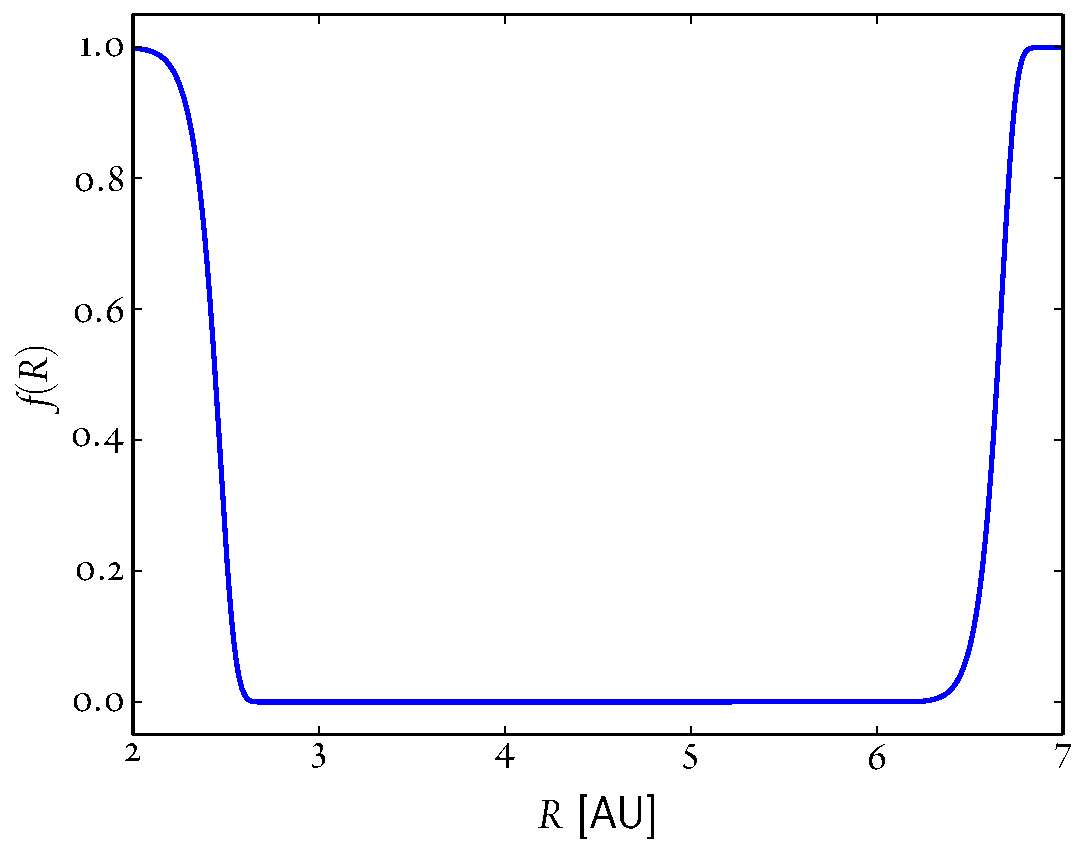
\includegraphics[width=0.5\textwidth]{figures/overlap}
   \caption{Przebieg funkcji $f(R)$ opisywanej równaniem~\mref{eq:overlap} dla
   zakresu promieni użytego we wszystkich symulacjach przedstawionych w~tej
pracy.}
   \label{fig:overlap}
\end{figure}
%
\subsection{Parametry symulacji}\label{ch2:simpar}
%
W~ramach pracy doktorskiej przeprowadzono szereg symulacji 2D modyfikując
początkowy $\epsilon$ oraz promień cząstek $a$, w~celu weryfikacji użytych metod
i wskazania optymalnych parametrów dla pełnych symulacji trójwymiarowych. Aby
móc porównać wyniki z~pracą innych autorów~\citep{JY07} parametr $\epsilon$
wybrano z~przedziału $[0.2, 2.0]$. Taki dobór parametru $\epsilon$ pozwala także
wzbudzić morfologicznie odmienny wyniki niestabilności strumieniowej, które
zostaną opisane w~dalszej części pracy. Promień cząstek pyłu został dobrany, tak
aby otrzymane wyniki można było porównać z~pracą JY, a także tak, aby były na
tyle małe aby ich obecność w~dysku protoplanetarnym można było wyjaśnić w~ramach
modelu zderzeniowego wzrostu przedstawionego w~rozdziale 1. Pełne zestawienie
użytych parametrów zostało przedstawione w~tabeli~\ref{tab1}.

\begin{table}
   \centering
   \begin{tabular}{cccccc}
      \hline
      Nazwa & $N_r \times N_\varphi \times N_z$ &
      $a$~[cm] & $\epsilon$ & $T_\textrm{end}$~[yr] \\
      \hline
      BD3d  &  $2560  \times 512 \times 192$  & 50  & 3.0 & 500  \\
      BD3dS &  $2560  \times 512 \times 192$  & 50  & 3.0 & 250  \\
      AA    &  $5120  \times 1   \times 300$  & 10  & 0.2 & 3000 \\
      AB    &  $5120  \times 1   \times 300$  & 10  & 1.0 & 3000 \\
      AC    &  $5120  \times 1   \times 300$  & 10  & 2.0 & 3000 \\
      BA    &  $5120  \times 1   \times 300$  & 50  & 0.2 & 3000 \\
      BB    &  $5120  \times 1   \times 300$  & 50  & 1.0 & 3000 \\
      BB3d  &  $2560  \times 512 \times 192$  & 50  & 1.0 & 500  \\
      BC    &  $5120  \times 1   \times 300$  & 50  & 2.0 & 3000 \\
      AAh   &  $10240 \times 1   \times 600$  & 10  & 0.2 & 1700 \\
      AAu   &  $20480 \times 1   \times 1200$ & 10  & 0.2 & 1800 \\
      ABh   &  $10240 \times 1   \times 600$  & 10  & 1.0 & 1400 \\
      BAh   &  $10240 \times 1   \times 600$  & 50  & 0.2 & 1730 \\
      BBh   &  $10240 \times 1   \times 600$  & 50  & 1.0 & 3000 \\
      \hline
   \end{tabular}
\caption{Parametry użyte w~symulacjach. Kolumny opisują w~kolejności: oznaczenie
   kodowe symulacji, ilość komórek obliczeniowych w~kierunkach $r$, $\varphi$ i
   $z$, promień cząstek, początkowy stosunek gęstości pyłu do gęstości gazu,
całkowity czas trwania symulacji w~latach.}
\label{tab1}
\end{table}

%%%%%%%%%%%%%%%%%%%%%%%%%%%%%%%%%%%%%%%%%%%%%%%%%%%%%%%%%%%%%%%%%%%%%%%%%%%%%%%%
% vim: tw=80 ts=3: 

\begin{savequote}[75mm]
   If I model a phenomenon accurately, does that mean I understand it? Or might it be simple coincidence, or an artifact
   of the technique? Of course, as an ardent simulationist, I myself put much faith in Engine-modeling.
\qauthor{Edward Mallory, The Difference Engine by William Gibson and Bruce Sterling}
\end{savequote}

\chapter{Wyniki}


%The following two sections describe
%different non-linear evolution of streaming instability in quasi-global setup
%with reference to similar case shown by JY07.

\section{Symulacje dwuwymiarowe}
Poniżej przedstawiono opis wyników uzyskanych dla symulacji w~przypadku
dwuwymiarowym. Ich celem, w~połączeniu z~liniową analizą stabilności, była
weryfikacja zaimplementowanych metod oraz poprawności przyjętego modelu. Każdy z
przedstawionych wyników można porównać do analogicznych eksperymentów
numerycznych z~pracy JY07~\cite{JY07}. Pomimo istotnych różnic w~użytych
metodach (JY stosowali kod wysokiego rzędu -- PENCIL, a także traktowali pył
jako cząstki materialne, a nie płyn), wyniki we wszystkich przypadkach wykazują
zgodność ilościową i~jakościową.

\subsection{Luźno związane ,,kamienie''}% ($a=50\,\textrm{cm}$, $\tau_s\approx
%1.2$)\label{marg_boulders}}

\begin{figure*}
   \centering
   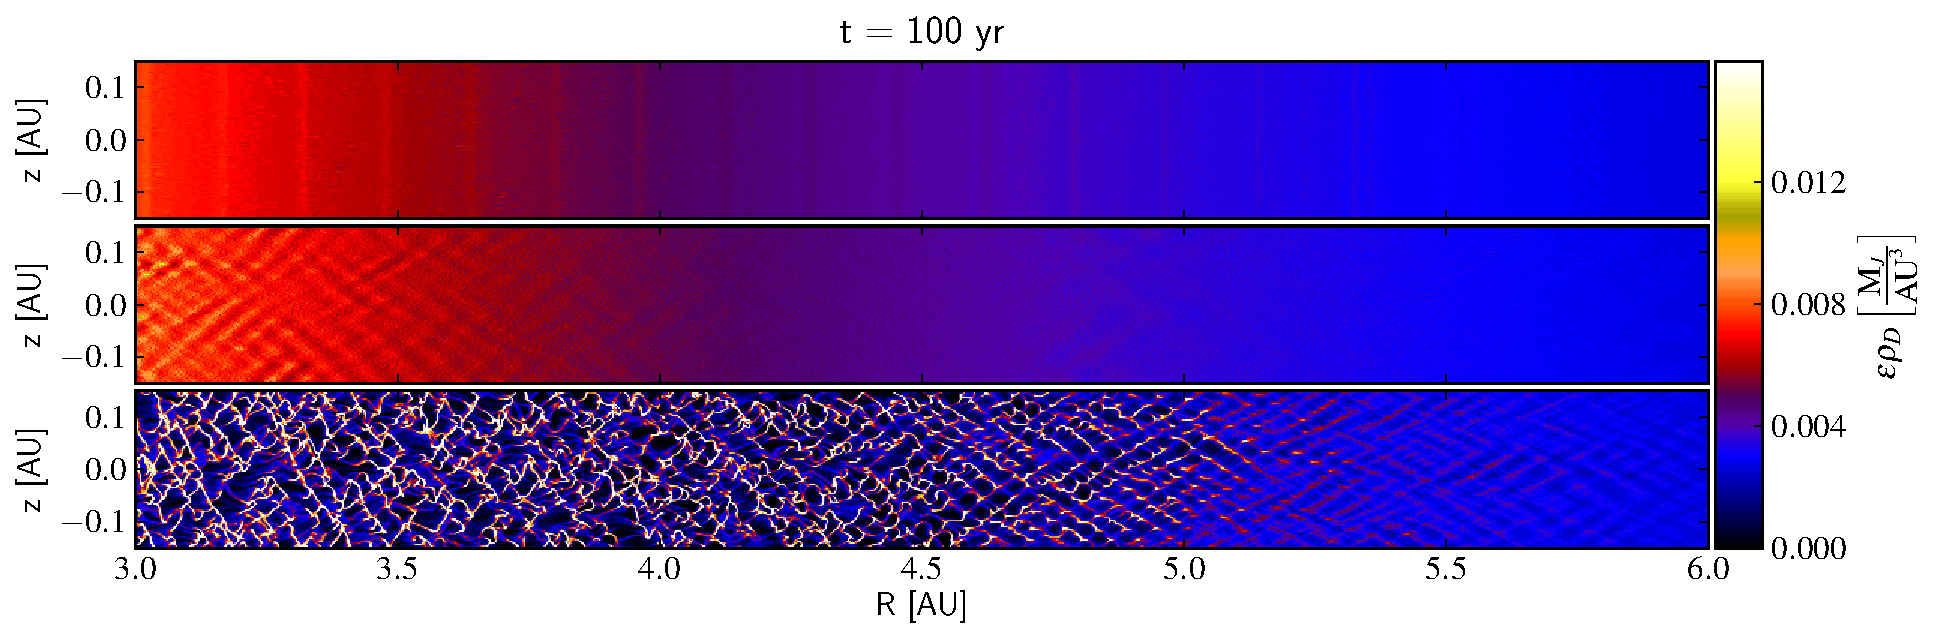
\includegraphics[width=0.99\linewidth]{figures/fig1a}
   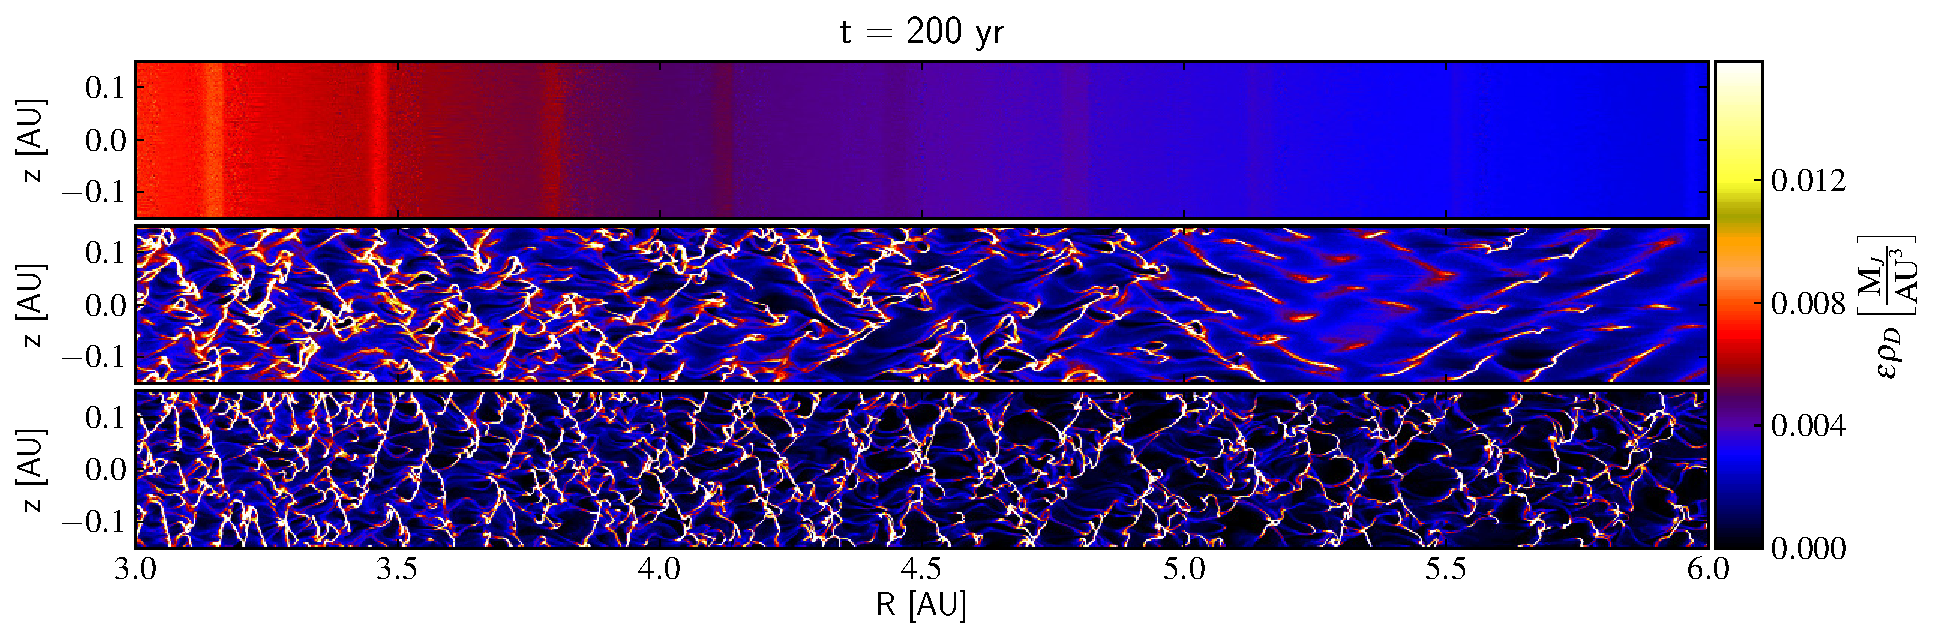
\includegraphics[width=0.99\linewidth]{figures/fig1b}
   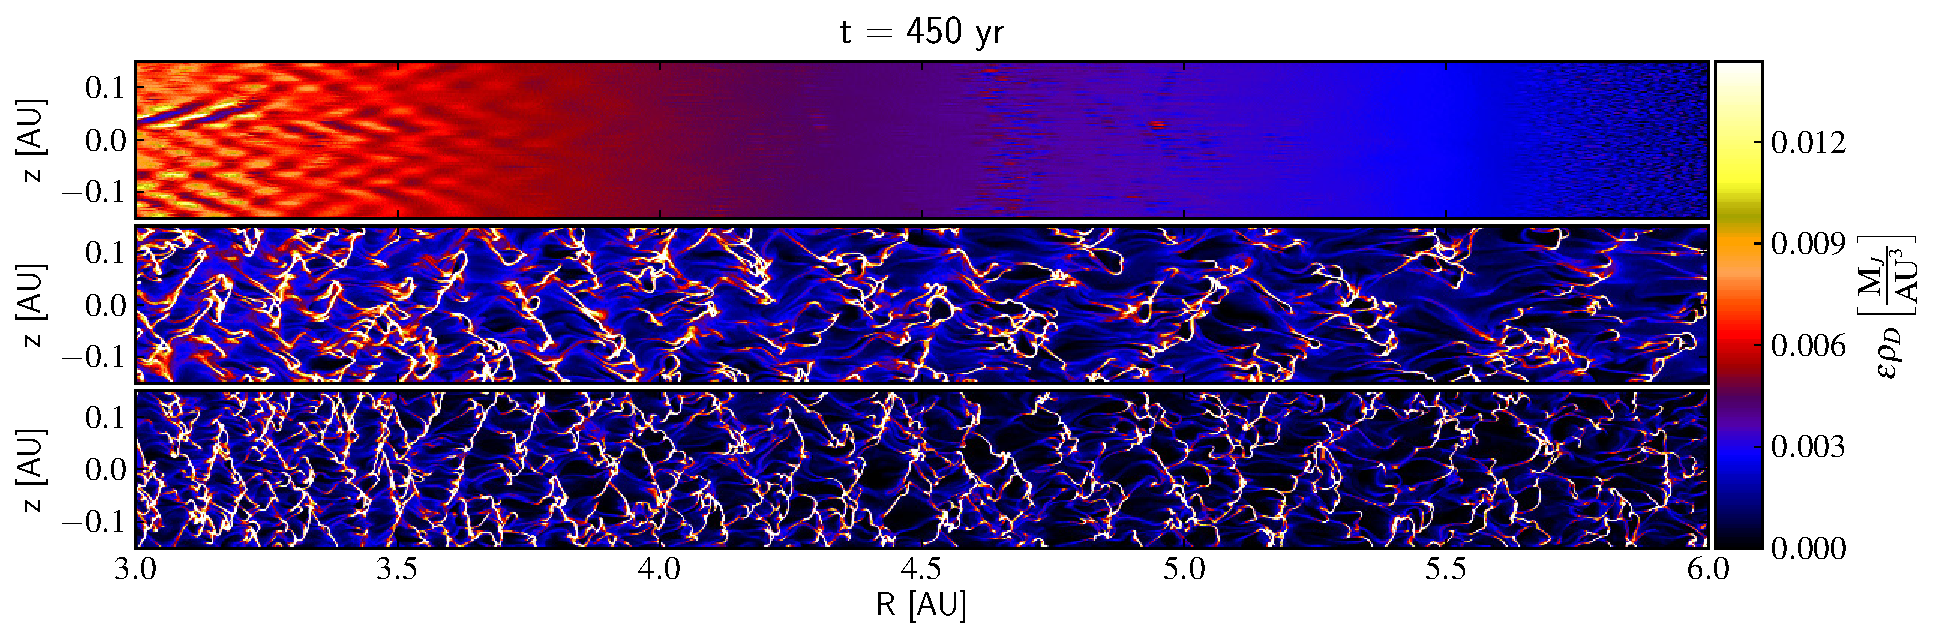
\includegraphics[width=0.99\linewidth]{figures/fig1c}
   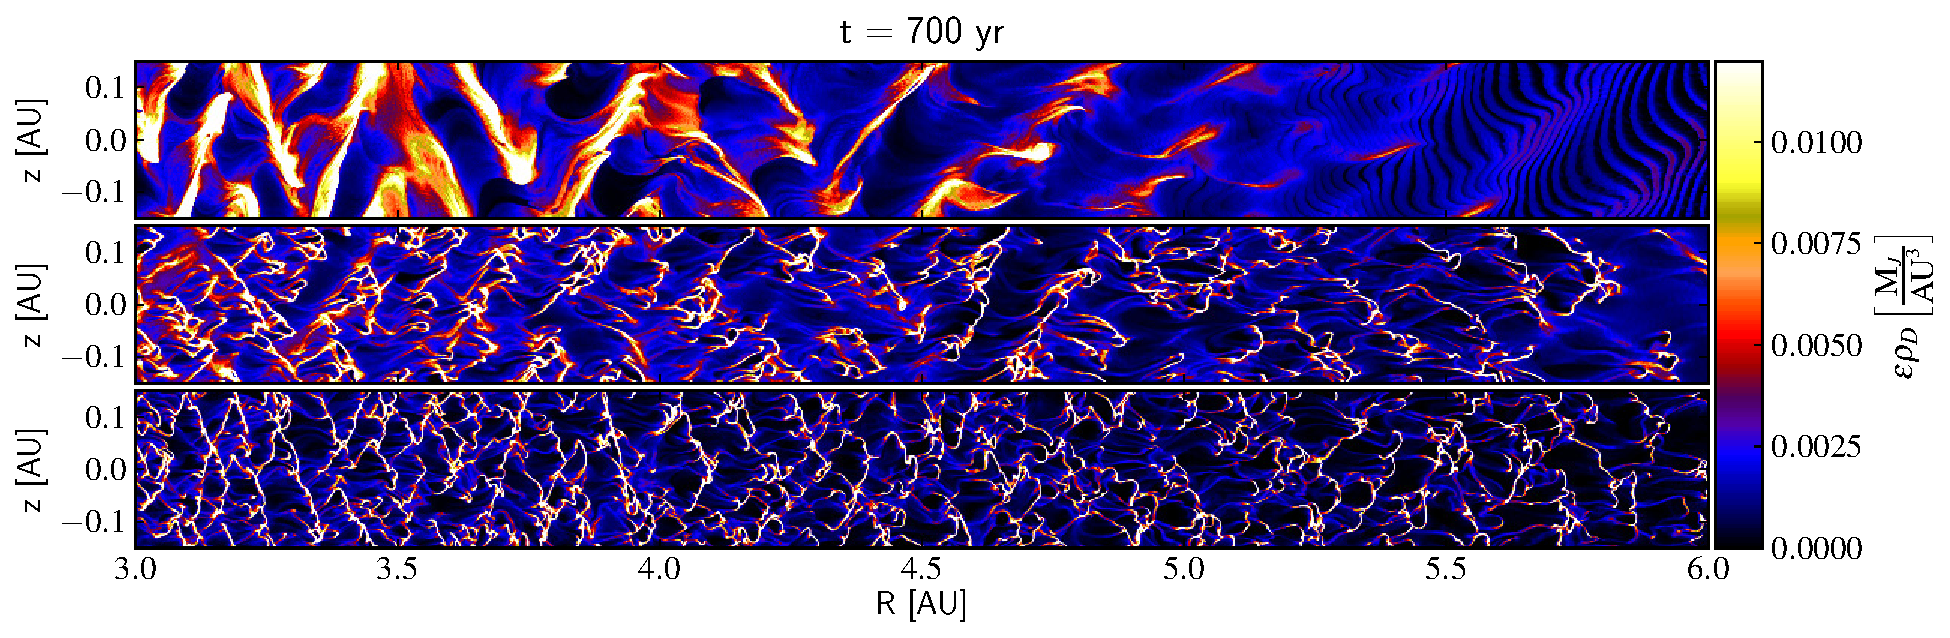
\includegraphics[width=0.99\linewidth]{figures/fig1d}
   \caption{Migawki gęstości pyłu dla symulacji z~$50$~cm ziarnami pyłu
      dla czasu $100$, $200$, $450$ oraz $700$~lat odpowiednio dla lewego
      górnego, prawego górnego, dolnego lewego i~dolnego prawego panelu.
      Każdy z~paneli jest podzielony na trzy części różniące się początkowym 
      $\epsilon = 0.2, 1, 2.0$ odpowiednio dla górnego (BAh), środkowego (BB) i
      dolnego (BC) podpanelu.}
   \label{fig1}
\end{figure*}
%

Niestabilność strumieniowa tworzy najbardziej prominentne struktury pyłu dla
cząstek pyłu o $\tau_s \sim 1$, czyli dla cząstek odsprzęgających się od
dynamiki gazu.
Przy wybranych parametrach symulacji opisanych w~rozdziale~\ref{ch2:simpar},
bezwymiarowy parametr ,,stopping time'' jest bliski jedności dla cząstek pyłu o
rozmiarach $50\cm$ (BA, BB, BC). Początkowa liniowa faza ewolucji jest
zdominowana przez wzrost gęstości dla najbardziej niestabilnych modów i~prowadzi
do znacznego wzrostu lokalnej gęstości pyłu i~uformowania się
charakterystycznych, wydłużonych diagonalnie włókien. W~rzeczywistości są to
spłaszczone struktury rozciągające się w~kierunku współrzędnej azymutalnej. Po
osiągnięciu nasycenia i~przejścia do nieliniowej ewolucji, włókna, na skutek
dużej prędkości w~kierunku wertykalnym ulegają fragmentacji i~wzajemnie się
przenikają. Jednakże pył dalej poruszą się po charakterystycznych
,,v''--kształtnych trajektoriach, które wytworzyły się podczas liniowej fazy
ewolucji. Migawki z~czasowej ewolucji gęstości pyłu zostały przedstawione na
obrazku~\ref{fig1}. Wyraźny jest wpływ początkowego stosunku gęstości pyłu do
gęstości gazu $\epsilon$ na morfologię formujących się obłoków: zarówno ich
typowy rozmiar, jak i~kąt nachylenia względem płaszczyzny dysku. Dla $\epsilon =
1$ pył poruszą się i~formuje struktury nachylone pod kątem $45^o$, dla
pozostałych przypadków $\epsilon=0.2, 2.0$ kąt nachylenia jest dużo większy,
przez co formujące się struktury są rozciągnięte w~kierunku \emph{z}. We
wszystkich wypadkach niestabilność strumieniowa prowadzi do lokalnego wzrostu
gęstości o prawie 2 rzędy wielkości.  Ze względu na swoją gęstość

\subsection{Mocno sprzężony ,,żwir''}
%($a=10\,\textrm{cm}$, $\tau_s\approx 0.24$)
%\label{tight_boulders}}
\begin{figure*}
   \centering
   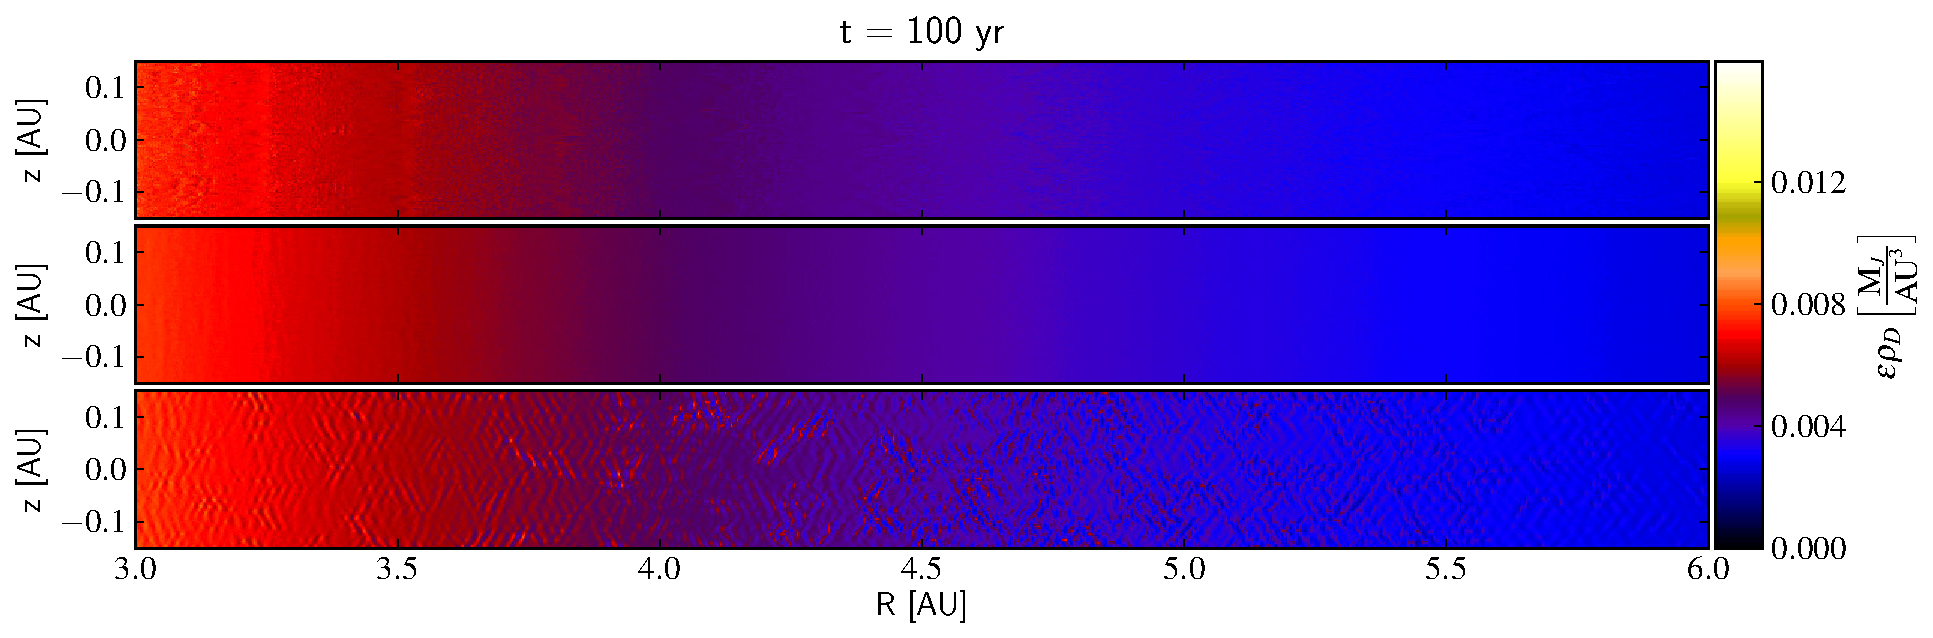
\includegraphics[width=0.99\linewidth]{figures/fig2a}
   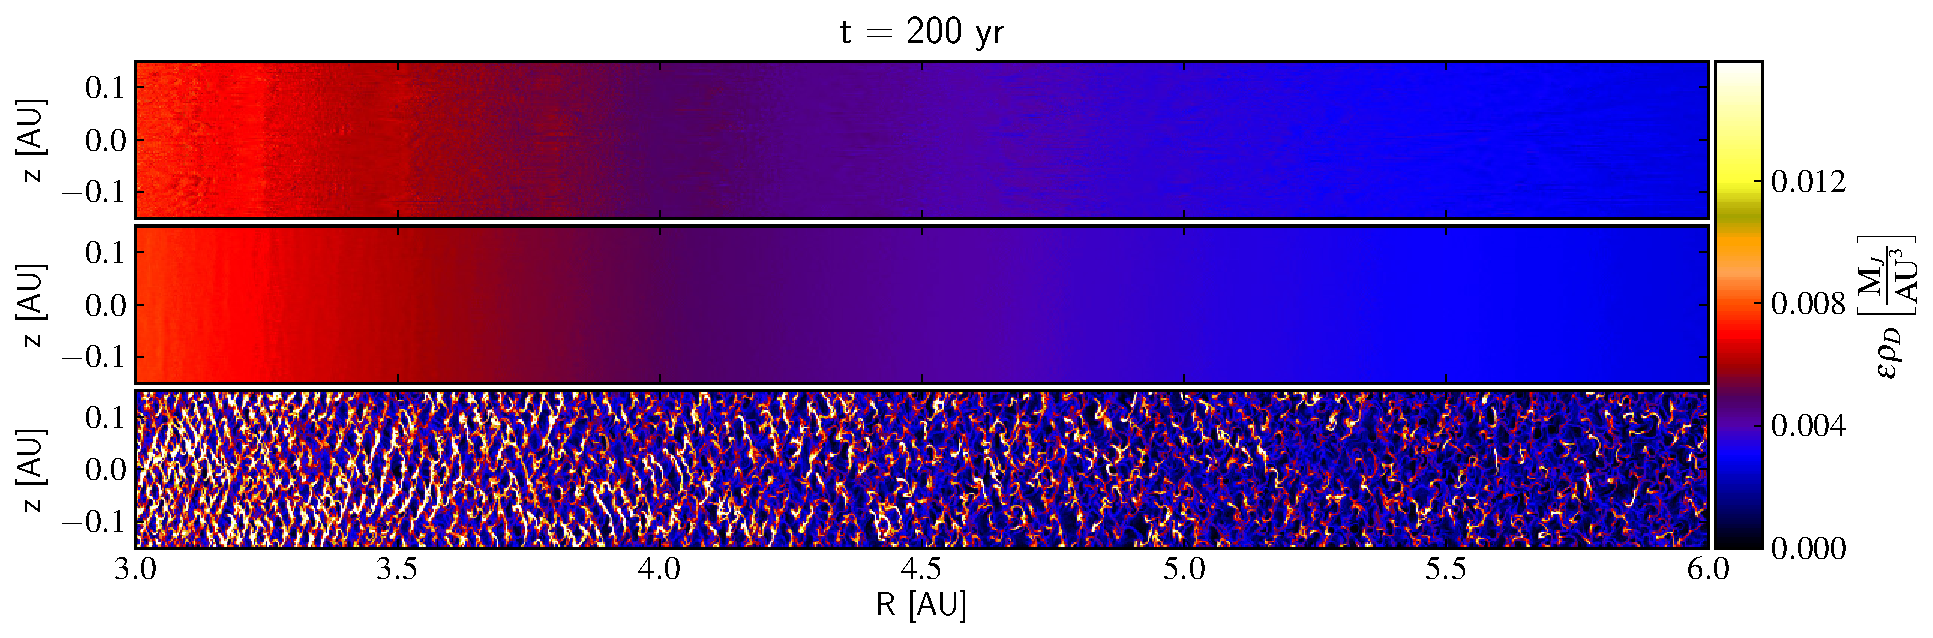
\includegraphics[width=0.99\linewidth]{figures/fig2b}
   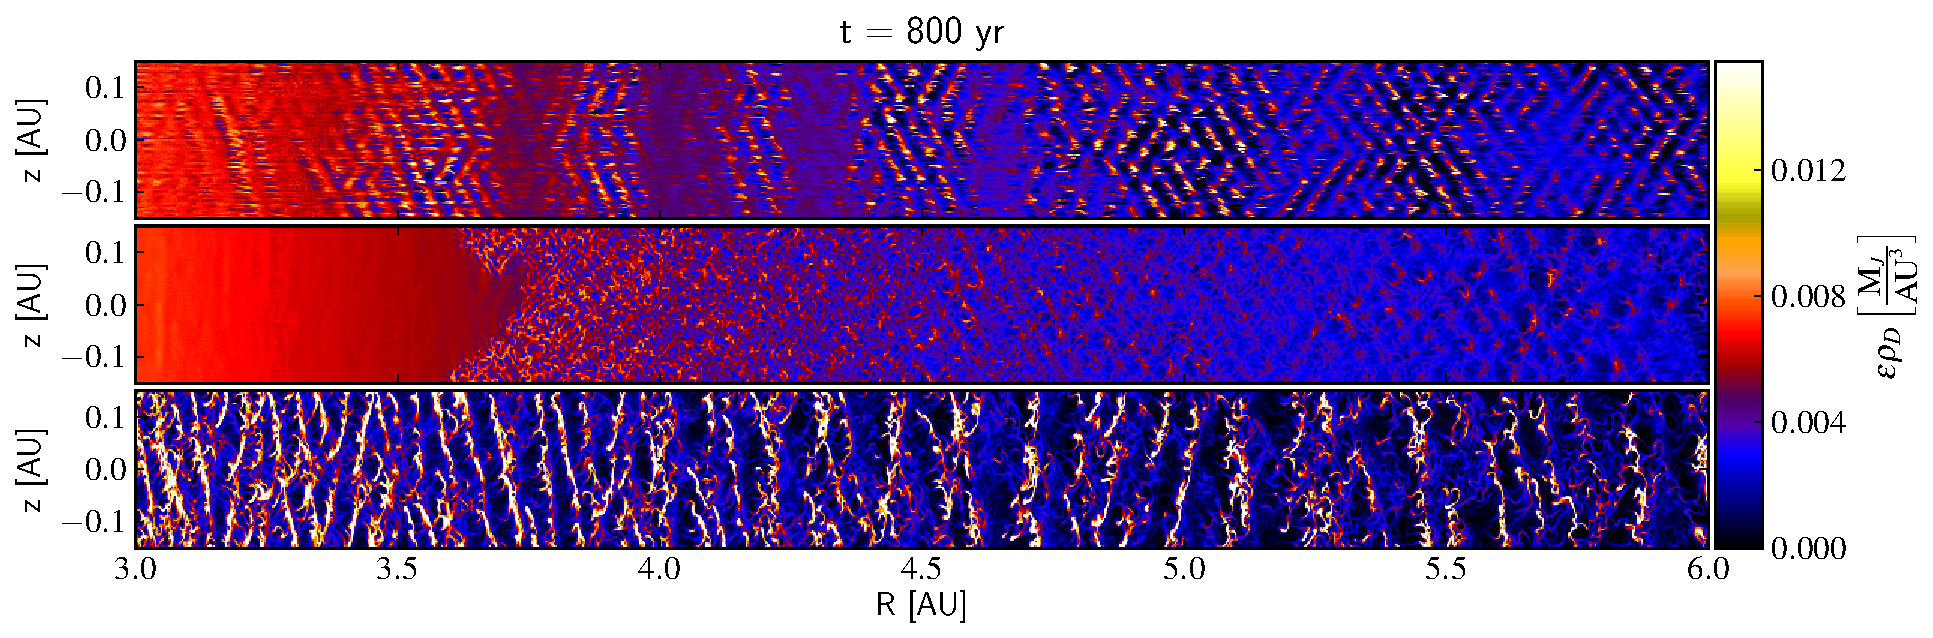
\includegraphics[width=0.99\linewidth]{figures/fig2c}
   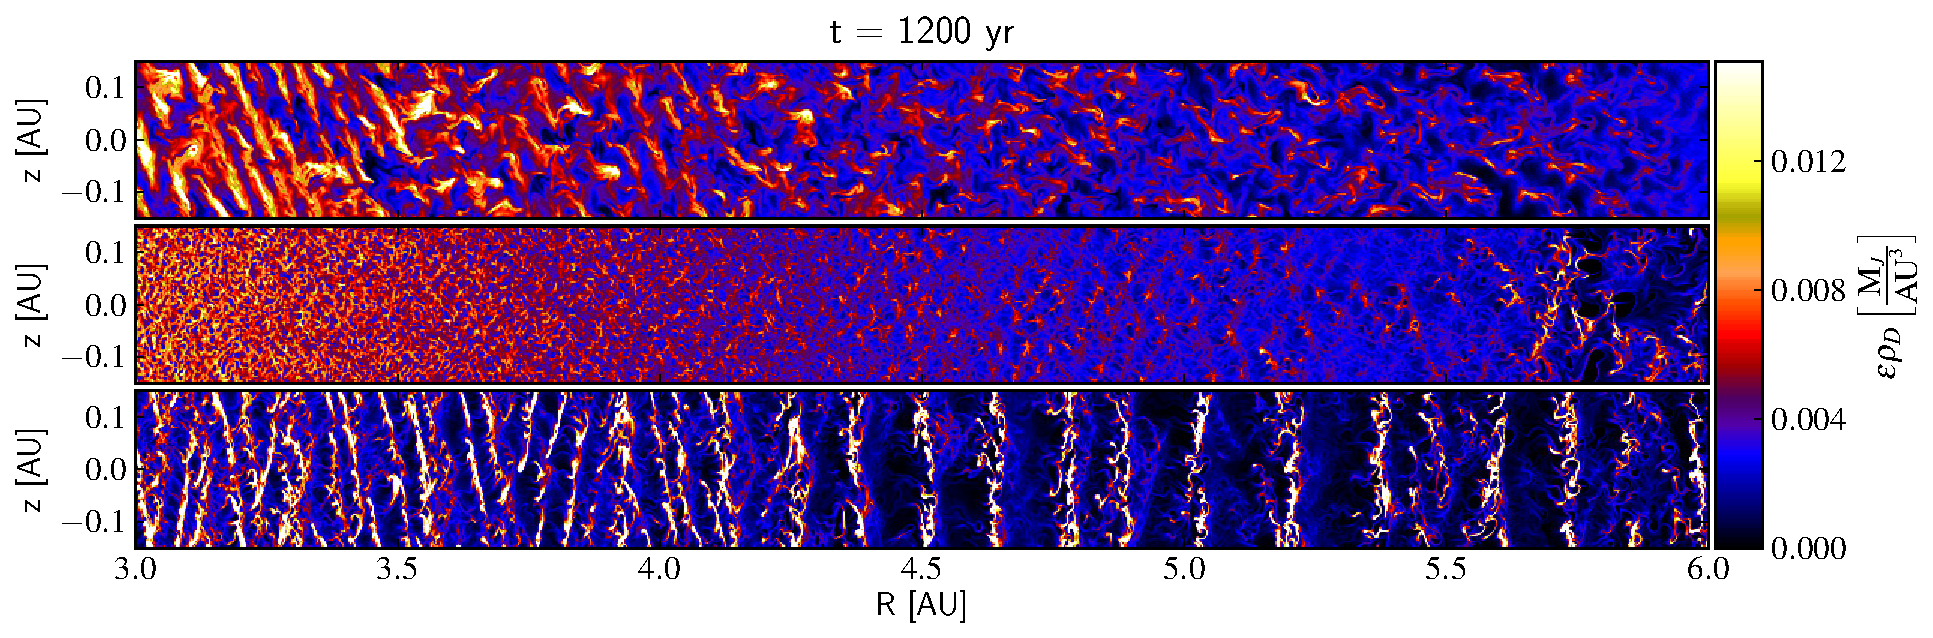
\includegraphics[width=0.99\linewidth]{figures/fig2d}
   \caption{Migawki gęstości pyłu dla symulacji z~$10$~cm ziarnami pyłu
      dla czasu $100$, $200$, $800$ oraz $1200$~lat odpowiednio dla lewego
      górnego, prawego górnego, dolnego lewego i~dolnego prawego panelu.
      Każdy z~paneli jest podzielony na trzy części różniące się początkowym 
      $\epsilon = 0.2, 1, 2.0$ odpowiednio dla górnego (AA), środkowego (AB) i
      dolnego (AC) podpanelu.}
   \label{fig2}
\end{figure*}
Czasowy przebieg symulacji dla silnie sprzężonego pyłu (AA - AC) został
przedstawiony na Rysunku~\ref{fig2}. Ewolucja pyłu dla przypadku $\epsilon =
2.0$ i~$10\cm$ ziaren pyłu (AC) nie odbiega znacząco od ewolucji analogicznego
przypadku dla $50\cm$ ziaren pyłu. Liniowa faza niestabilności podczas której
pył zostaje zagęszczony dla najbardziej niestabilnych modów, prowadzi do
wytworzenia się struktur wydłużonych w~kierunku wertykalnym. Ze względu na
mniejsze tempo migracji dla sprzężonych cząstek pyłu, zagęszczenia są pochylone
w kierunku radialnym tylko w~niewielkim stopniu. Maksymalna gęstość pyłu nie
przekracza dwudziestokrotności wartości początkowej.
\par Przypadek $\epsilon = 0.2$ charakteryzuje się niskim tempem wzrostu. W
początkowej liniowej fazie wzrost lokalnej gęstości pyły prowadzi do uformowania
się charakterystycznej diagonalnej siatki zagęszczeń. Lokalne maksima gęstości
sięgają nawet stukrotnej wielokrotności gęstości początkowej. Jednakże, przejście
do fazy nieliniowej prowadzi do gwałtownego rozmycia skupisk pyłu i~osiągnięcia
quasi-stacjonarnego stanu, w~którym zagęszczenia podlegają silnej turbulencji,
zaś ich maksymalna amplituda nie przekracza jednego rzędu wielkości względem
stanu początkowego (por. Rysunek~\ref{fig4}).

\par Najciekawszym przypadkiem, zasadniczo odbiegającym od pozostałych, jest
symulacja AB ($\epsilon=1.0,\, a=10\cm$). Początkowo ewolucja przebiega w
identyczny sposób jak dla pozostałych warunków, tzn. pojawia się regularny wzór
w gęstości pyłu odpowiadający najbardziej niestabilnym długościom fal. Jednakże 
po $800$~latach w~symulacji AB (mniej więcej dwa razy szybciej w~symulacji ABh)
pojawiają się gwałtownie rozszerzające się bąble wypełnione nie wielką ilością
pyłu, które silnie koncentrują pył na swoich brzegach (por. Rysunek~\ref{fig3}). 
Znacząco wzrasta prędkość z~którą porusza się pył, po okresie kilkuset lat
silnie turbulentne ruchy propagują się na całą domenę obliczeniową. Ta
specyficzna ewolucja niestabilności strumieniowej jest spowodowana odmiennym
przebiegiem liniowego tempa wzrostu niestabilności (patrz Rysunek~\ref{fig2b})
Dla ustalonych parametrów fizycznych AB tempo wzrostu niestabilności $s$ wypada
w punkcie przegięcia funkcji $s(\epsilon)$. Lokalne zwiększenie $\epsilon$ o
tylko $\sim10\%$ przekłada się na dwukrotne zwiększenie tempa wzrostu. Powoduje
to, że drobne zagęszczenia lokalne osiągają nieliniową fazę ewolucji dużo
szybciej niż mniej gęste obszary.  Jest to bezpośrednim powodem obserwowanego
zjawiska, które YJ określili mianem ,,kawitacji''~\footnote{jako analog
gwałtownego pojawiania się bardzo rzadkich bąbli pyłu do nagłego przejścia z
fazy ciekłej do gazowej}.  Turbulencja w~pyle prowadzi do wytworzenia się
lokalnych zagęszczeń sięgających rząd wielkości ponad stan początkowy. Jest to
zgodne z~wynikami przedstawionymi przez JY07 (patrz Rysunek.~8 w~Ich pracy).

\begin{figure} 
\centering
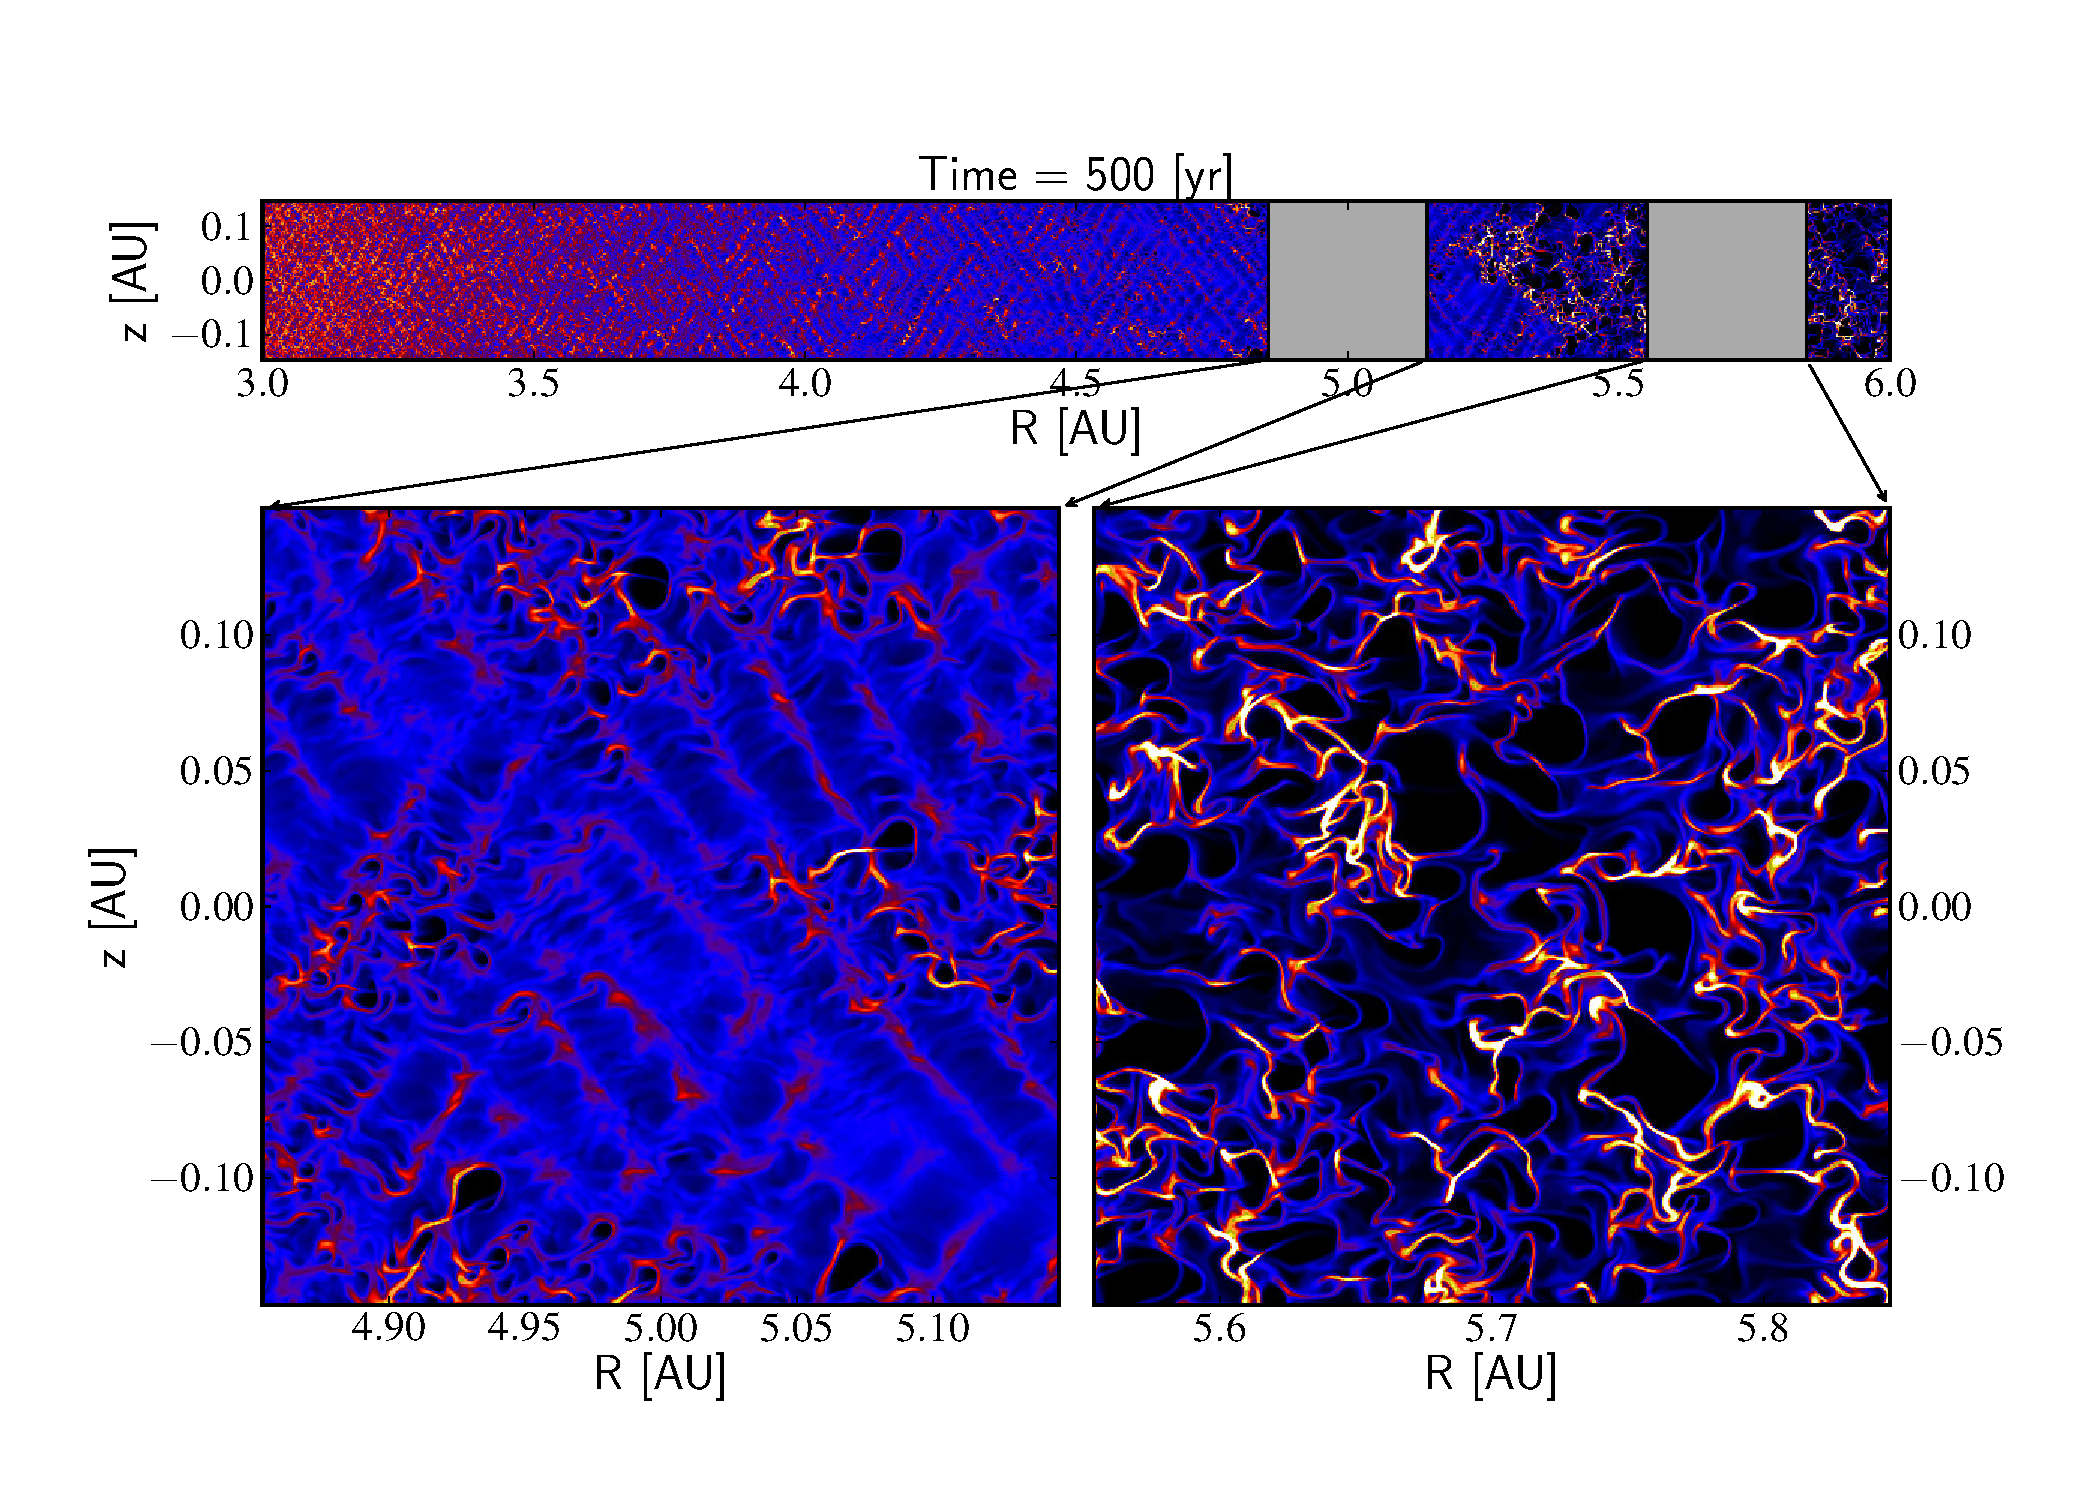
\includegraphics[width=0.98\linewidth]{figures/fig3}
\caption{Migawki gęstości gazu dla symulacji ABh pokazujące dwa ,,zbliżenia''
   obszarów gdzie: występuje pseudo-kawitacja wynikająca z~lokalnych zagęszczeń
   wytworzonych w~liniowej fazie wzrostu (lewy panel) oraz region całkowicie
   opanowany przez wybuchające bąble pustki i~silną turbulencję pyłu (prawy
   panel). Animacja przedstawiająca ewolucję symulacji ABh jest dostępna pod
   adresem \href{http://youtu.be/NoA5-TiQabQ}{http://youtu.be/NoA5-TiQabQ}.}
\label{fig3}
\end{figure}

\begin{figure}
   \centering
   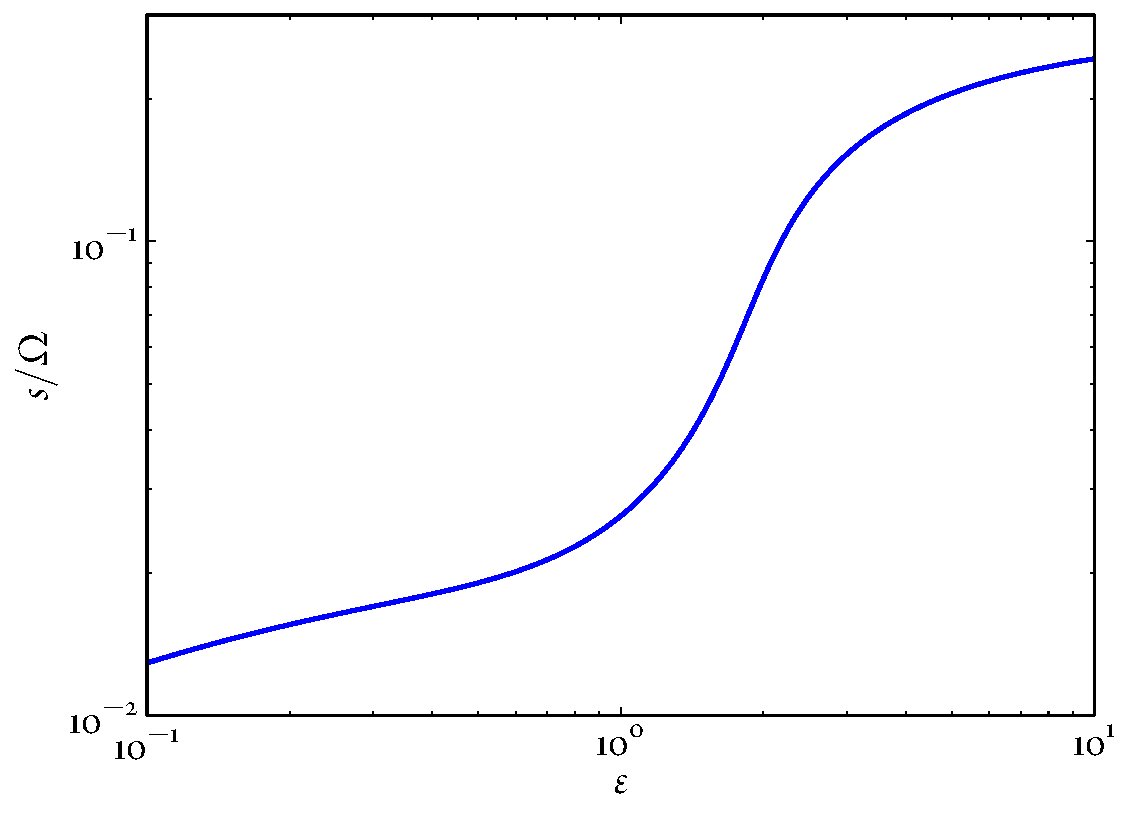
\includegraphics[width=0.5\linewidth]{figures/growthAB}
   \caption{Liniowe tempo wzrostu niestabilności strumieniowej jako funkcja
      stosunku gęstości pyłu do gęstości gazu. Pozostałe parametry niezbędne do
      rozwiązania równania~\mref{eq:disprel} zostały wzięte obszaru znajdującego
   się na lewym panelu Rysunku~\ref{fig2}.}
   %Przełamanie przebiegu funkcji dla
   %   $\epsilon\sim 1$ jest bezpośrednim powodem ,,kawitacji'' obserwowanej w
   %   symulacji AB}
   \label{fig2b}
\end{figure}


\begin{figure}
   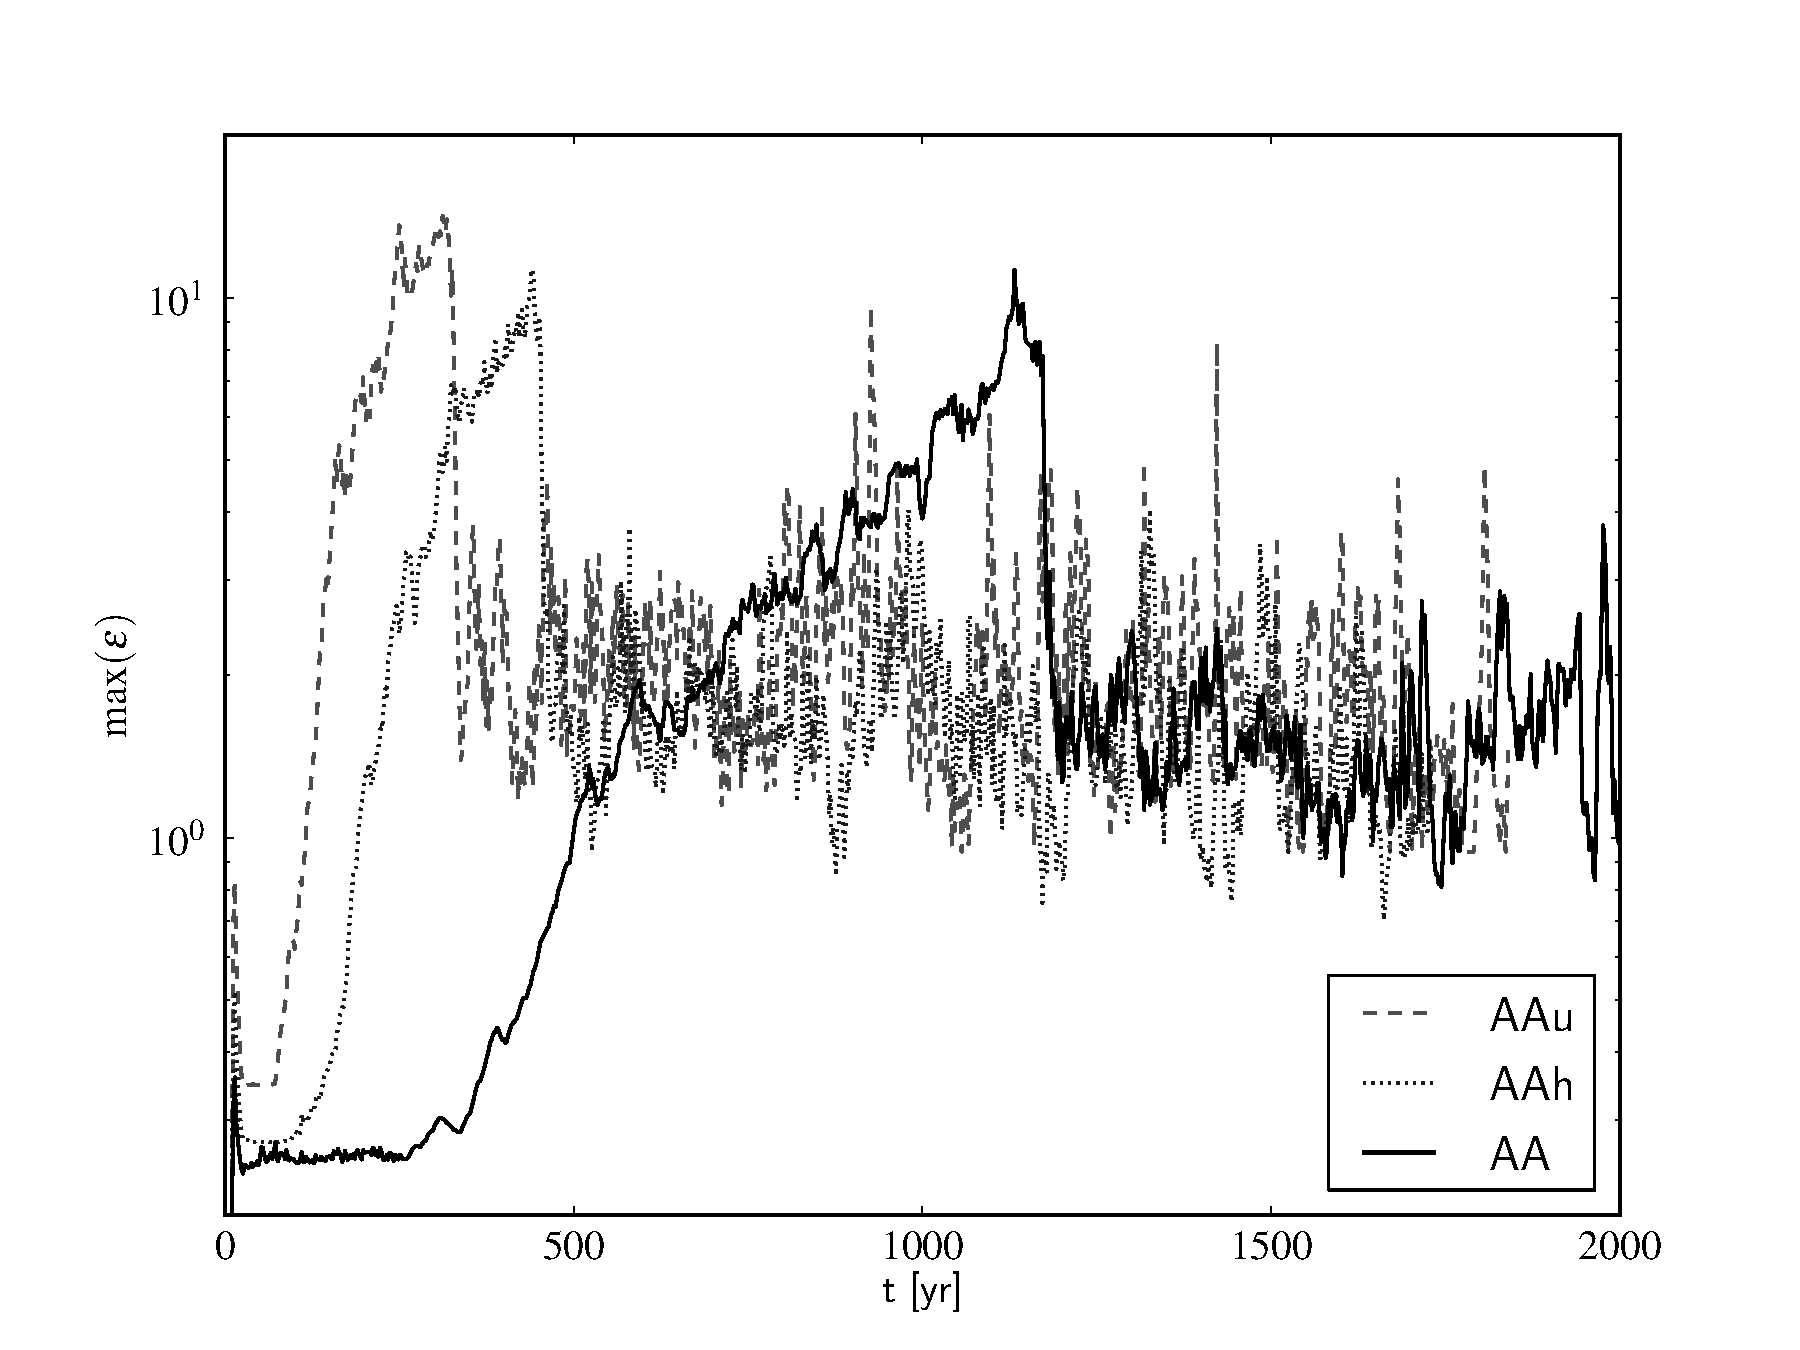
\includegraphics[width=0.98\linewidth]{figures/fig4}
   \caption{
      Maksymalne stosunek gęstości pyłu do gęstości gazu dla trzech symulacji z
      identycznymi, fizycznymi warunkami początkowymi, lecz różną
      rozdzielczością. Ewolucja niestabilności strumieniowej przebiega według
      scenariusza: (1) szybki wzrost podczas liniowej fazy ewolucji, który
      zwiększa lokalnie $\epsilon$ o dwa rzędy wielkości, (2) po
      osiągnięciu krytycznego $\epsilon\approx 10$, zagęszczenia pyłu zostają
      gwałtownie rozmyte, (3) niestabilność osiąga wysycenie, nieliniowa
      ewolucja sprowadza się do oscylacji gęstości pyłu w~postaci dużych,
      rozmytych obszarów o maksymalnej gęstości nieprzekraczającej
      dziesięciokrotności wartości początkowej. Zmiana rozdzielczości nie ma
      wpływu na powyższy scenariusz, jedynie wprowadza krótsze i~szybciej
   rosnące długości fal skracając etap (1).}

   \label{fig4}
\end{figure}
%

\section{Porównanie wyników z~liniową analizą stabilności}
\label{sec:simulation_analysis}
Aby móc porównać obserwowane tempa wzrostu niestabilności strumieniowej z
analizą przedstawioną w~rozdziale~\ref{sec:lsa} z~domeny obliczeniowej
wyodrębniono małe, kwadratowe ,,łatki'' na wybranych orbitach. Rozmiar wybranych
obszarów $(0.15^2\AU)$ pozwala traktować je w~ramach lokalnego przybliżenia
kostki ścinanej, a także umożliwia wyrażenie stałych parametrów występujących w
równaniach \mref{lin1}--\mref{lin4}) poprzez wartości średnie w~łatce.
Można zatem przyjąć, że $\bar{\rho}_g = \left<\rho_g\right>$, $\bar{\rho}_d =
\left<\rho_d\right>$ to średnie przestrzenne odpowiednio gęstości gazu i
gęstości pyłu, oraz że ich średni wzajemny stosunek to $\bar{\epsilon} =
\left<\rho_d / \rho_g\right>$. Jako Średnią częstość kątowa $\bar{\Omega}$
przyjęto częstość kątową środka łatki. Bezwymiarowa miara podkeplerowskiej
rotacji jest obliczona zgodnie ze wzorem (patrz YG05 rów.~(16) albo JY07
rów.~(1)).  Wypadku trójwymiarowych symulacji, które dokładnie zostaną opisane
w kolejnych częściach tego rozdziału, ,,łatka'' została wybrana w
płaszczyźnie {\it r-z} dla $\varphi = \varphi_\textrm{max} / 2$.
%
\begin{equation}
   \bar{\eta} = -\frac{c_s^2\left<\partial_R \left<\rho_g\right>_z\right>_R}
      {2\bar{\rho}_g\bar{\Omega}^2 R},
   \label{eq:meaneta}
\end{equation}
%
W~równaniu~\mref{eq:meaneta} średnia z~gęstości gazu jest liczona najpierw w
kierunku wertykalnym, a następnie jest obliczana średnia z~radialnej pochodnej 
$\left<\partial_R \rho_g\right>$. Wyrażenie na średni ,,stopping time'' zostało
wyprowadzone z~równania~\mref{eq:tauf}
\begin{equation}
   \bar{\tau}_f = \rho_\bullet a / \left(\bar{\rho}_g \sqrt{c_s^2 +
   \left<\left|\mathbf{u} - \mathbf{v}\right|^2\right>} \right).
\end{equation}
%
Dla spójności średnie prędkości gazu i~pyłu $\bar{\mathbf{u}},
\bar{\mathbf{w}}$ również są brane jako średnie wartości
$\left<\mathbf{u}\right>, \left<\mathbf{w}\right>$ zamiast obliczania ich przy
pomocy równań~\mref{eq:w0}-\mref{eq:u0} wynikających z~założenia dodatkowego
członu w~równaniach, niezbędnego w~przybliżeniu kostki ścinanej. 
Należy zauważyć, że wartości $\left<\mathbf{u}\right>, \left<\mathbf{w}\right>$,
osiągnięte w~sposób naturalny w~trakcie trwania symulacji, nie różnią się od
wartości analitycznych o więcej niż $10\%$.
\par Aby określić liniowe tempo wzrostu dla wzbudzanych modów niestabilności
rozkład gęstości i~prędkości poszczególnych płynów został przekształcony przy
pomocy transformaty Fouriera, tak aby uzyskać informację o amplitudach
wzbudzanych fal. Analiza przebiegu czasowego zmienności amplitud dla
poszczególnych częstości pozwala wyizolować najbardziej niestabilne mody układy.
Ten etap analizy dla jednej z~łatek został przedstawiony na Rysunku~\ref{fig7}.

\begin{figure}
  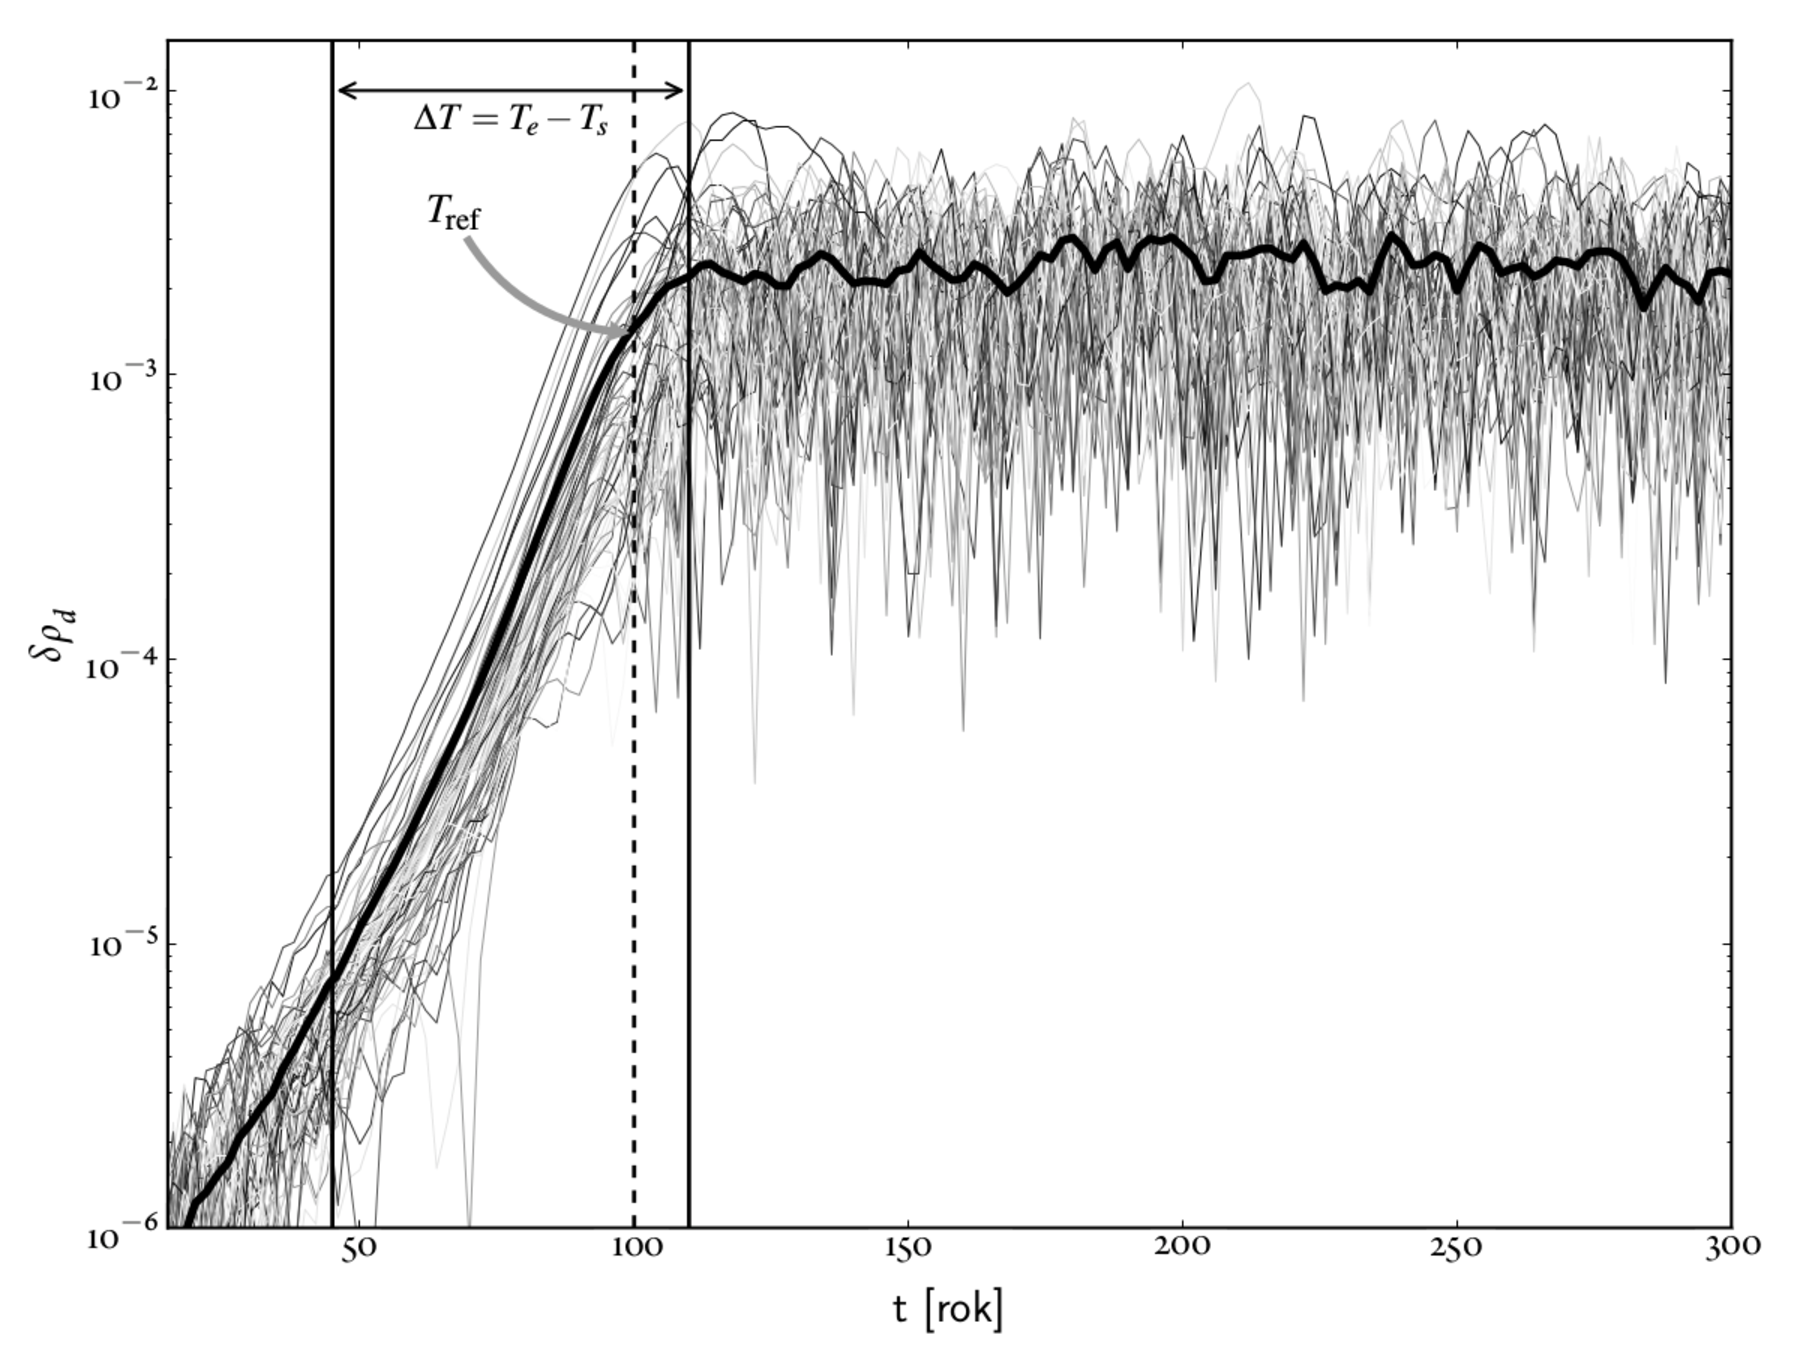
\includegraphics[width=0.98\linewidth]{figures/fig7}

  \caption{Czasowa ewolucja amplitud zaburzenia gęstości pyłu w~przestrzeni
     fourierowskiej dla łatki z~symulacji BB obejmującej obszar 
     $[2.85,3.15]\times[-0.15,0.15]~\AU^2$. Każda cienka, szara linia
     reprezentuje amplitudę dla wybranej pary liczb falowych $k_x, k_z$.
     $\Delta T = T_e - T_s$ to odcinek czasu dla którego do modów jest
     dopasowywane równanie~\mref{eq:fit}. $T_{\textrm{ref}}$ to punkt
     odniesienia dla którego identyfikowane są dominujące mody na podstawie
     wartości maksymalnej amplitud. Gruba, czarna linia pokazuje uśredniony
     przebieg zmienności dla modów, których amplituda dla $t = T_{\textrm{ref}}$
     jest większa niż $10^{-4}$.} 
   \label{fig7} 
\end{figure}

Dla każdego z~badanych obszarów określono czas $T_s$ dla którego część modów
zaczyna wyłaniać się z~szumu i~rozpoczyna fazę liniowego wzrostu. Na
podobnej zasadzie wyznaczono czas $T_e$, dla którego następuje wysycenie
wzrostu. Następnie do wszystkich modów na przedziale $\Delta T = T_e - T_s$
zostaje dopasowana funkcja
%
\begin{equation}
   f(t) = A\exp\left(-s t\right).
   \label{eq:fit}
\end{equation}
%
Powyższa procedura pozawala na określenie tempa wzrostu w~funkcji liczb falowych
$s(k_x, k_z)$ dla wszystkich modów podczas ich liniowego wzrostu. Mody rosnące
najszybciej są określane poprzez znalezienie modów o najwyższej amplitudzie w
wybranym momencie czasu $T_{\textrm{ref}} \lesssim T_e$, tuż przed ich
saturacją. Żadnej z~wielkości: $T_s$, $T_e$, $T_{\textrm{ref}}$ nie da się
określić w~jednoznaczny sposób. Dla każdej łatki z~osobna były one dobierane
arbitralnie na podstawie wizualnej oceny przebiegu dużej ilości modów (patrz
rysunek~\ref{fig7}).  Po określeniu ich tempa wzrostu $s(k_x, k_z)$ jest ono
porównywane z~tempem wzrostu $s_0(k_x, k_z)$ wynikającym bezpośrednio z~liniowej
analizy dla średnich wielkości płynowych w~łatce.

\par Rysunek~\ref{fig8} pokazuje czasową ewolucję amplitud zaburzenia gęstości
pyłu dla 3 najszybciej rosnących modów, wraz z~dopasowaną funkcją~\mref{eq:fit}
i tempem wzrostu wynikającym z~liniowej analizy dla symulacji BB3d, BB oraz BBh.
Wyraźnie widoczny jest wpływ rozdzielczości na numeryczne tempo wzrostu, a także
zbieżność wyników eksperymentu numerycznego z~przewidywaniami teoretycznymi. W
najniższej rozdzielczości tempo wzrostu jest $10\div30\%$ mniejsze niż tempo
analityczne. Ostateczny poziom saturacji dla poszczególnych symulacji znajduje
się na różnym poziomie, ale należy zwrócić uwagę na fakt, że wzrost
rozdzielczości powoduję pojawienie się coraz to krótszych fal, które mogą rosnąć
szybciej i~zmieniać obraz całkowity niestabilności strumieniowej.
 
\begin{figure} 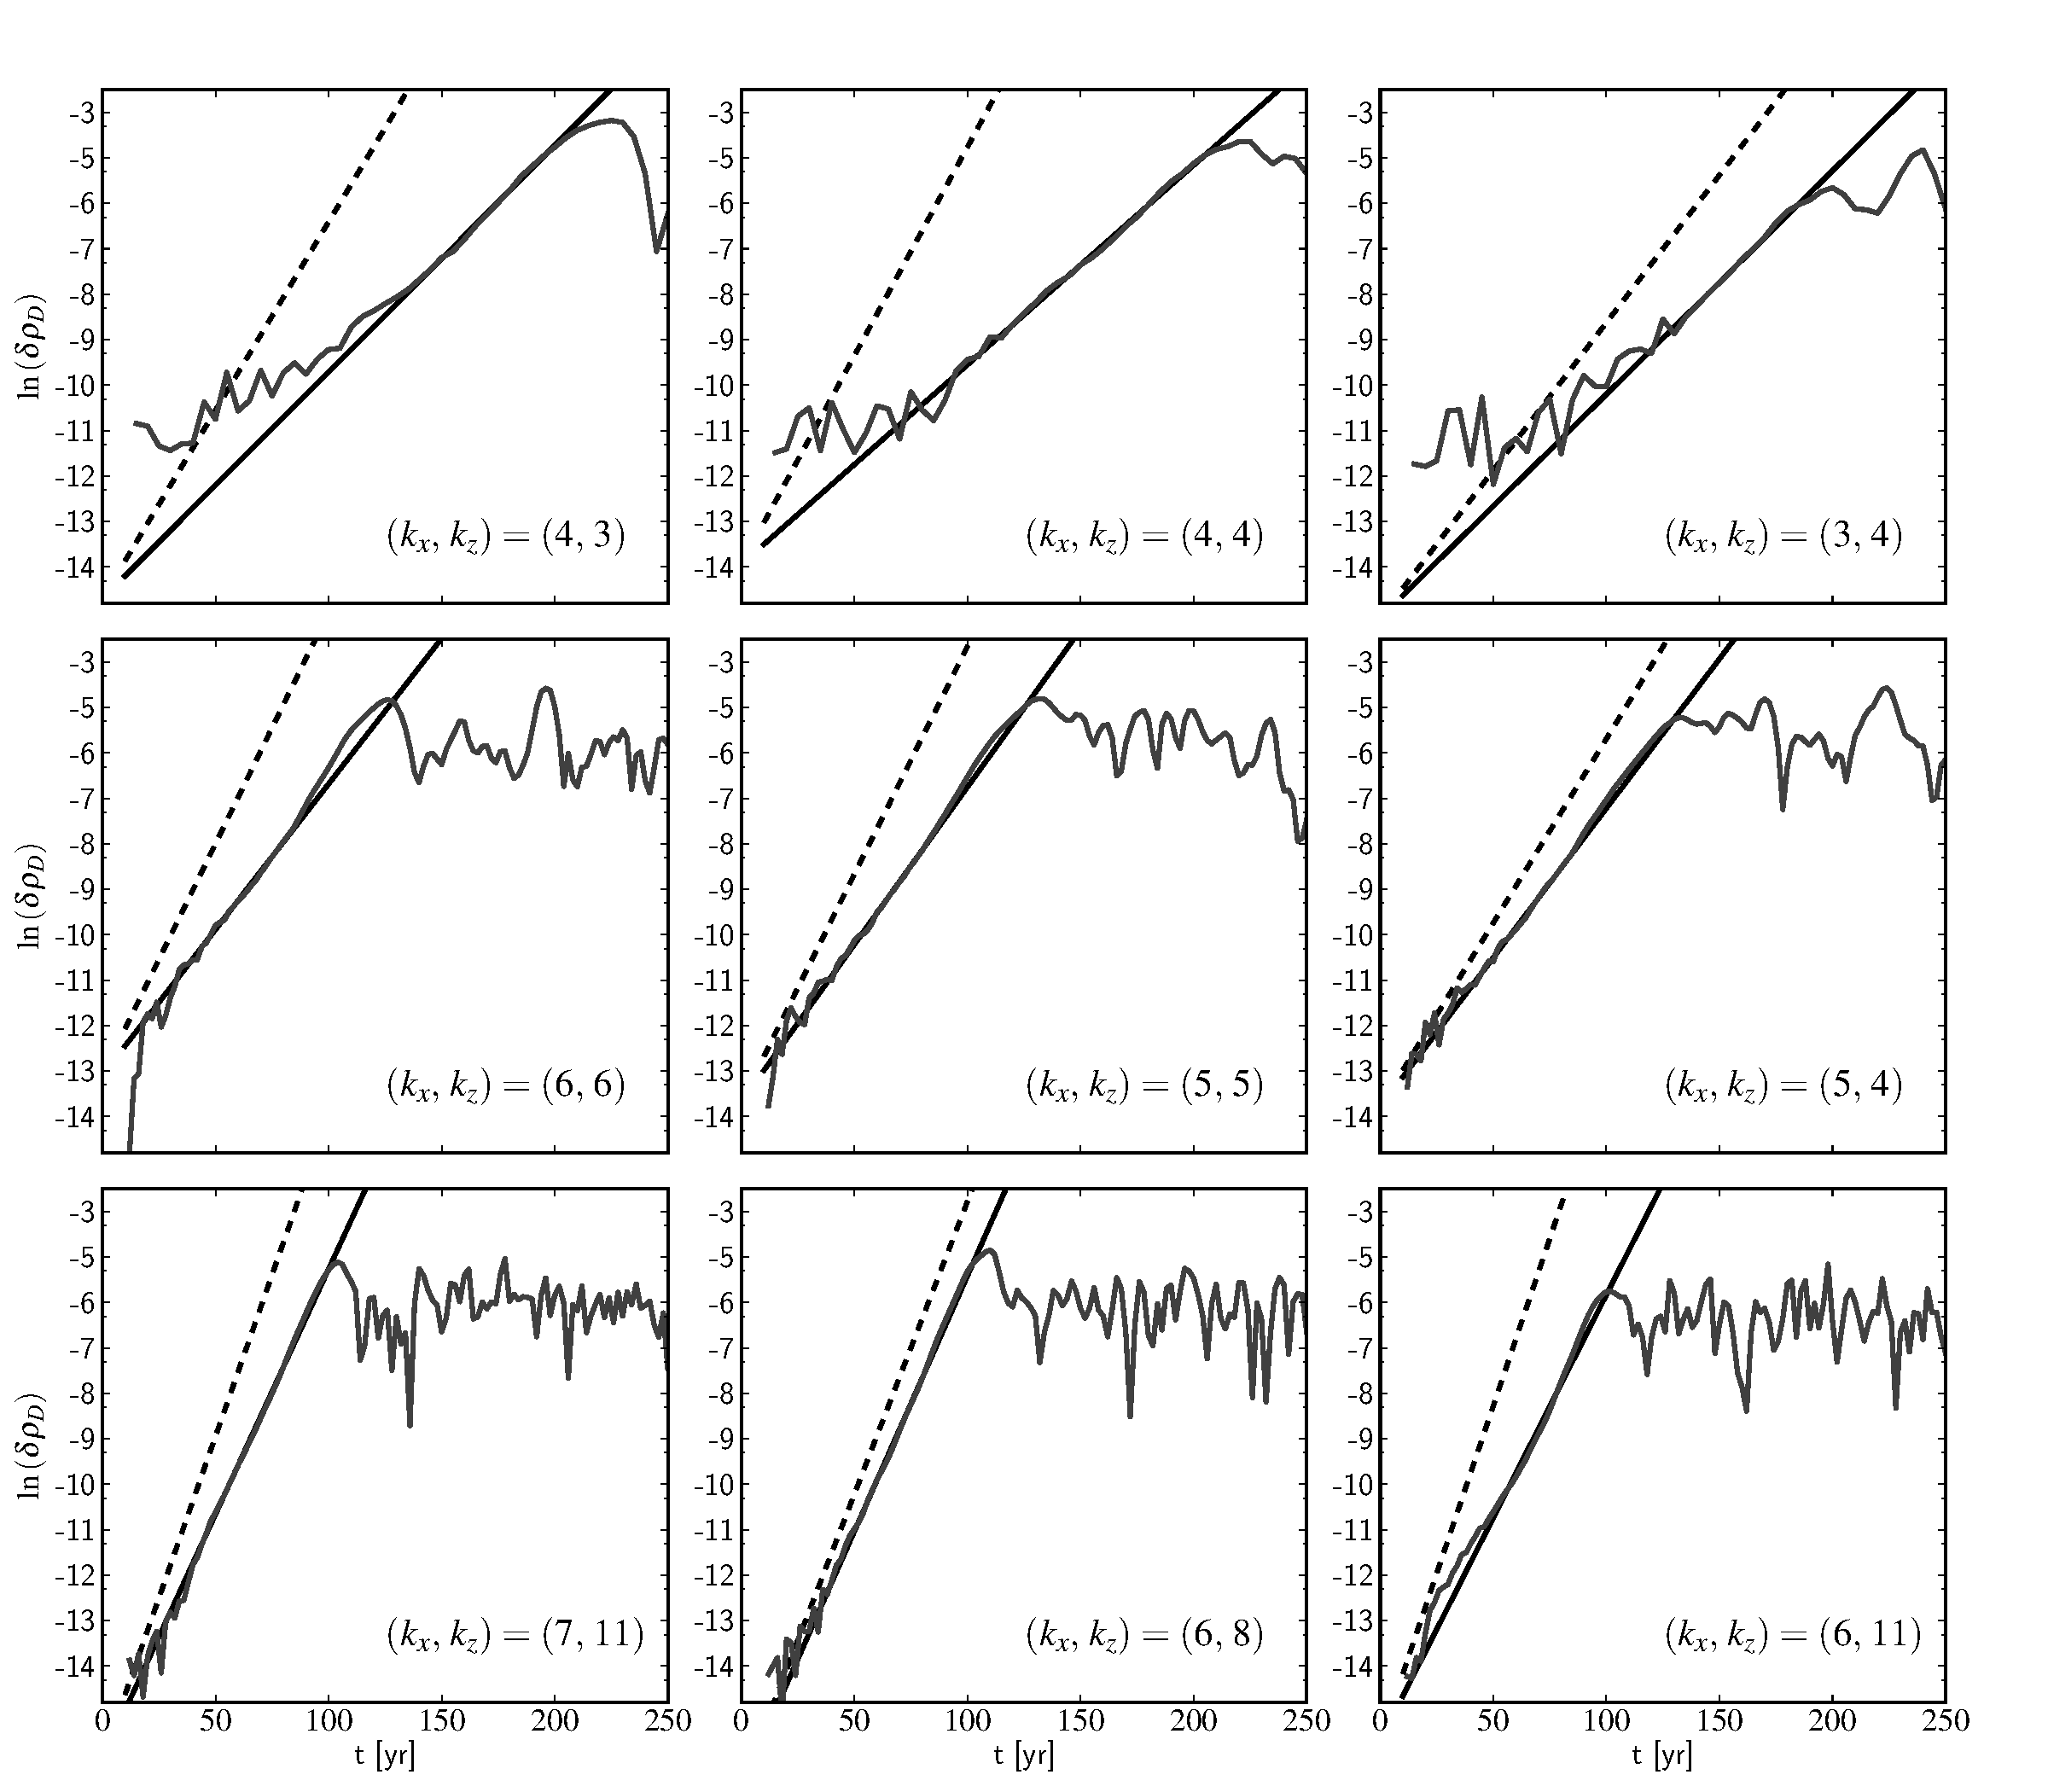
\includegraphics[width=0.98\linewidth]{figures/fig8}
   \caption{Czasowa ewolucja amplitud dominujących modów niestabilności
      strumieniowej mierzona dla zaburzenia gęstości (szara linia) wraz z
      dopasowaniem~\mref{eq:fit} (czarna linia) i~przewidywanym tempem wzrostu
      wynikającym z~liniowej analizy stabilności (linia przerywana).
      Rozwiązanie równania~\mref{eq:linset} jest określone na podstawie
      parametrów średnich kwadratowej łatki ulokowanej na $R=3\AU$ dla symulacji
BB3d (górny panel), BB (środkowy panel) and BBh (dolny panel).  } \label{fig8}
\end{figure}

\par Kolejnym argumentem potwierdzającym zgodność wyników z~liniową analizą
stabilności jest przedstawiony na Rysunku~\ref{fig9} wykres konturowy tempa
wzrostu wynikający z~rozwiązania równania~\mref{eq:disprel} w~zależności od
liczby falowej. Wyraźnie widać na nim, że najszybciej rosnące mody
niestabilności strumieniowej układają się w~charakterystyczny grzbiet w~kierunku
rosnących $k_x$ i~$k_z$.  Wykres tworzony jest dla stanu średniego w~łatce dla
czasu $T_{\textrm{ref}}$.  Następnie 9 dominujących modów wybranych wedle
kryterium opisywanego wcześniej jest zaznaczane przy użyciu punktów. Procedura
jest powtarzana dla symulacji o tych samych parametrach początkowych, ale
różnych rozdzielczościach.  Powyższy schemat działania pozwala potwierdzić, że
liczby falowe dominujących modów wzbudzanych w~eksperymencie numerycznym,
układają wzdłuż wspomnianego wcześniej grzbietu. Jedynym czynnikiem
ograniczającym wzrost modów krótkofalowych jest niewystarczająca rozdzielczość
domeny obliczeniowej. Dla serii symulacji BB3d, BB, BBh efektywna rozdzielczość
siatki wyniosła odpowiednio $150^2, 300^2, 600^2$ komórek obliczeniowych.
Dominujące mody symulacji o najniższej rozdzielczości grupują się poniżej
konturu ''$(-1.0)$'', zaś dla najwyższej praktycznie wszystkie mają tempo
wzrostu powyżej $0.1$. Podobne zachowanie jest widoczne dla pozostałych
symulacji dla których przeprowadzono testy zbieżności, tj. AB, ABh (prawy panel
na rysunku~\ref{fig9}). Przypuszczalnym powodem obecności wyraźnego obcięcia dla
krótki długości fali w~przeprowadzonych symulacjach jest wewnętrzną, numeryczna
dyfuzyjność metody RTVD użytej w~PIERNIKu. Z przeprowadzonych analiz wynika, że
używane algorytmy numeryczne potrzebują przynajmniej 32 komórek obliczeniowych
na długość fali niestabilnego modu, aby poprawnie oddać jego tempo wzrostu.
Należy przy tym zauważyć, że krótsze mody zawierające się w~mniejszej liczbie
komórek nadal pozostają niestabilne, aczkolwiek mogą wykazywać mniejsze tempo
wzrostu niż to wynikające z~liniowej analizy stabilności.

\begin{figure*}
  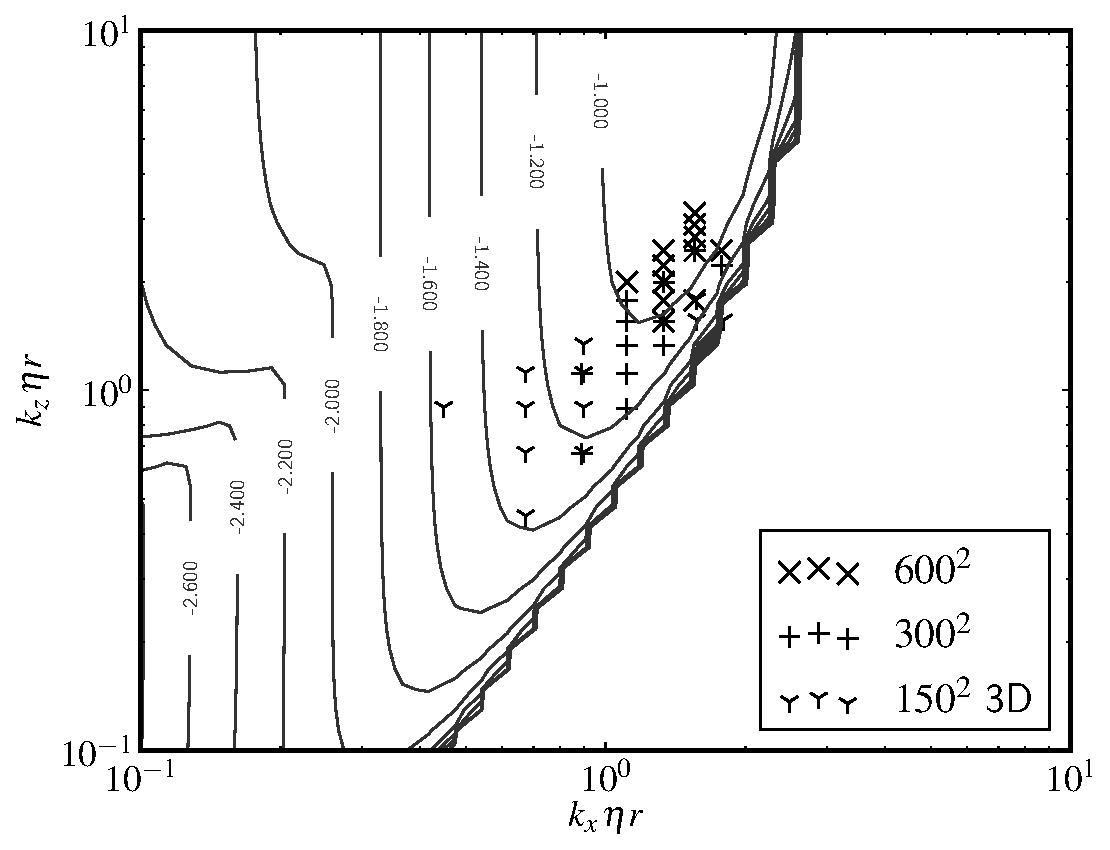
\includegraphics[width=0.48\linewidth]{figures/fig9a}
  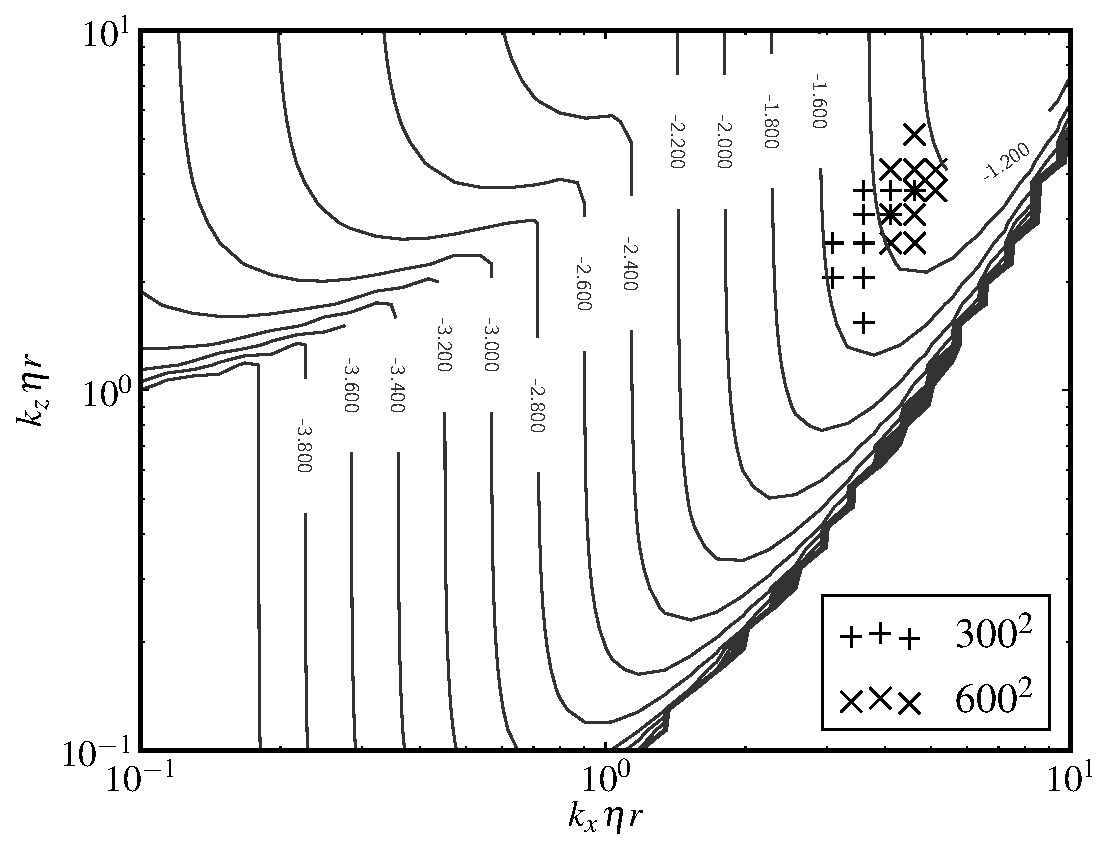
\includegraphics[width=0.48\linewidth]{figures/fig9b}
  \caption{Dziewięć najszybciej rosnących modów o liczbach falowych $(k_x, k_z)$
     wyodrębnionych z~symulacji o tych samych fizycznych warunkach początkowych,
     lecz różnej rozdzielczości siatki obliczeniowej. (lewy panel: BB3d, BB,
     BBh, prawy: AB, ABh). Kontury wyznaczają tempo wzrostu $\log_{10}( s_0(k_x,
  k_z))$ wynikające z~rozwiązania równania~ \mref{eq:disprel} dla średniego
  stanu wybranych łatek w~momencie czasu  $T = T_{\textrm{ref}}$ (dla porównania
  por. Rysunek.~2 z~pracy~\cite{YG05})}
   \label{fig9}
\end{figure*}
 
% \subsection{Convergence}
\par Jako że niestabilność strumieniowa w~ogólności ,,preferuje'' krótsze
długości fali, zwiększenia rozdzielczości zawsze prowadzi do wytworzenia
to zagęszczeń o coraz mniejszych rozmiarach w~krótszym czasie~(por.
Rysunek~\ref{fig10}).  Jednakże przeprowadzone symulacje odtwarzają w~dobrym
stopniu przewidywania liniowej analizy stabilności, a także są w~stanie oddać
wszystkie efekty jakościowe, np. ,,kawitację'' (por. Rysunek~\ref{fig3}) czy
gwałtowne rozmycie niestabilności w~przypadku $\epsilon=0.2$ i~$a=10\cm$, bez
względu na rozmiar najmniejszej komórki obliczeniowej.

\begin{figure}
   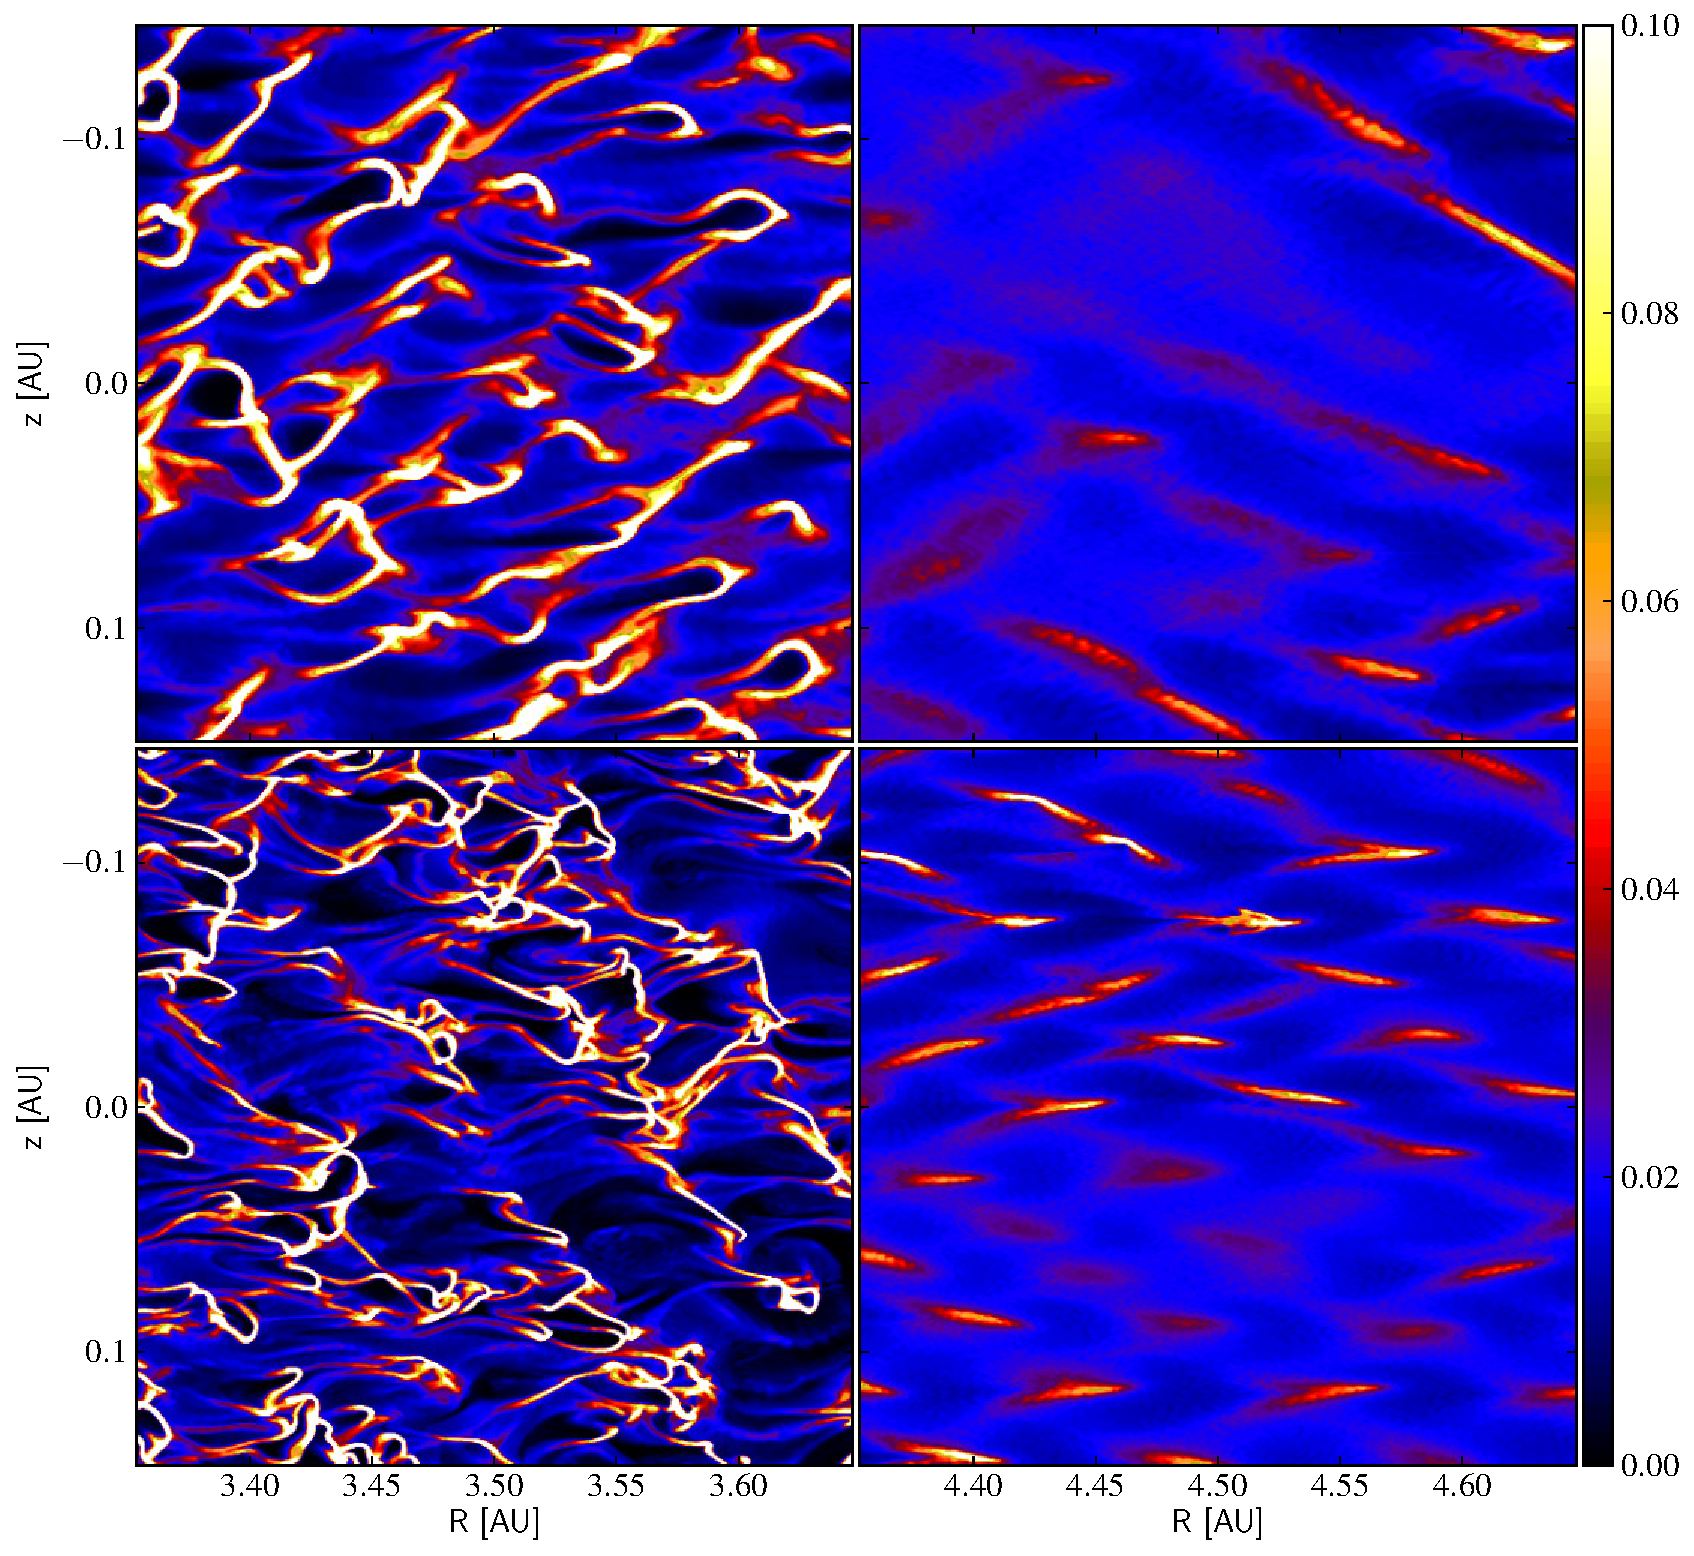
\includegraphics[width=0.98\linewidth]{figures/fig10}
   \caption{Migawki gęstości pyłu dla $t = 160\yr$ dla łatek pochodzących z
      orbit $R=3.5$ i~$4.5\AU$ wyodrębnione z~symulacji o tych samych warunkach
      początkowych lecz różnej rozdzielczości siatki obliczeniowej. Górny panel
      symulacja BB, zaś dolny symulacja BBh. Ze względu na właściwości
      dyfuzji numerycznej, wyższa rozdzielczość promuje krótsze długości
      fali}
   \label{fig10} 
\end{figure}

\section{Symulacje trójwymiarowe}
W~ramach poniższej pracy przeprowadzono 2 rodzaje symulacji pełnego,
trójwymiarowego modelu dysku: z~uwzględnieniem efektów samograwitacji płynów
(BD3dS) oraz bez jej udziału (BB3d, BD3d). Symulacja BB3d została przeprowadzana
w celu ścisłego porównania wyników z~analogicznymi symulacjami dwuwymiarowymi.
Podobnie jak w~przypadku zredukowanym, ewolucja niestabilności strumieniowej
przebiega głównie w~płaszczyźnie \textit{r-z}. Początkowo w~gęstości pyłu
wyłania się przedstawiony już wcześniej ukośny wzór, będący wynikiem działania
najbardziej niestabilnych modów. Wydłużone zagęszczenia pyłu formują warstwy
rozciągające się na cały dysk w~kierunku azymutalnym. Odstępstwa od osiowej
symetrii są zauważalne, lecz praktycznie nie wpływają na zachowanie się
niestabilności (por. Rysunek~\ref{fig:slicenosg}. Podobnie jak w~analogicznych
symulacjach 2D, saturacja niestabilności następuje po lokalnym wzroście gęstości
pyłu o $1\div1.5$ rzędu wielkości.
%
\begin{figure}
   \centering
   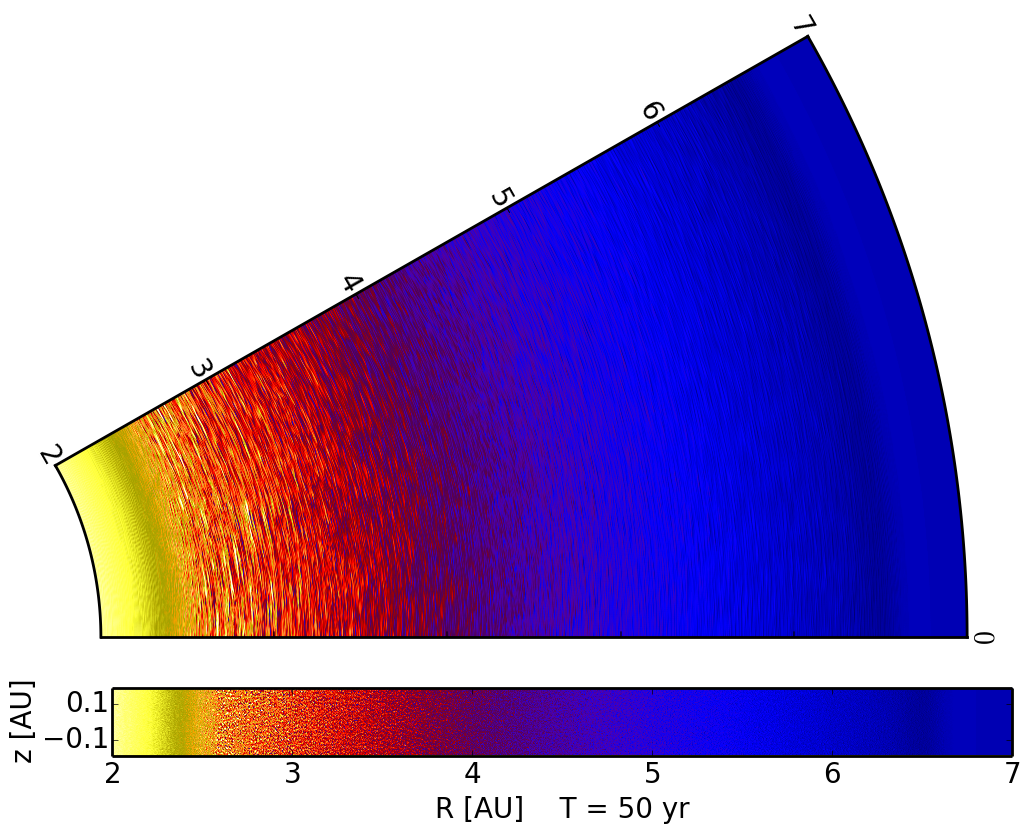
\includegraphics[width=0.44\linewidth]{figures/slice_nosg_01}
   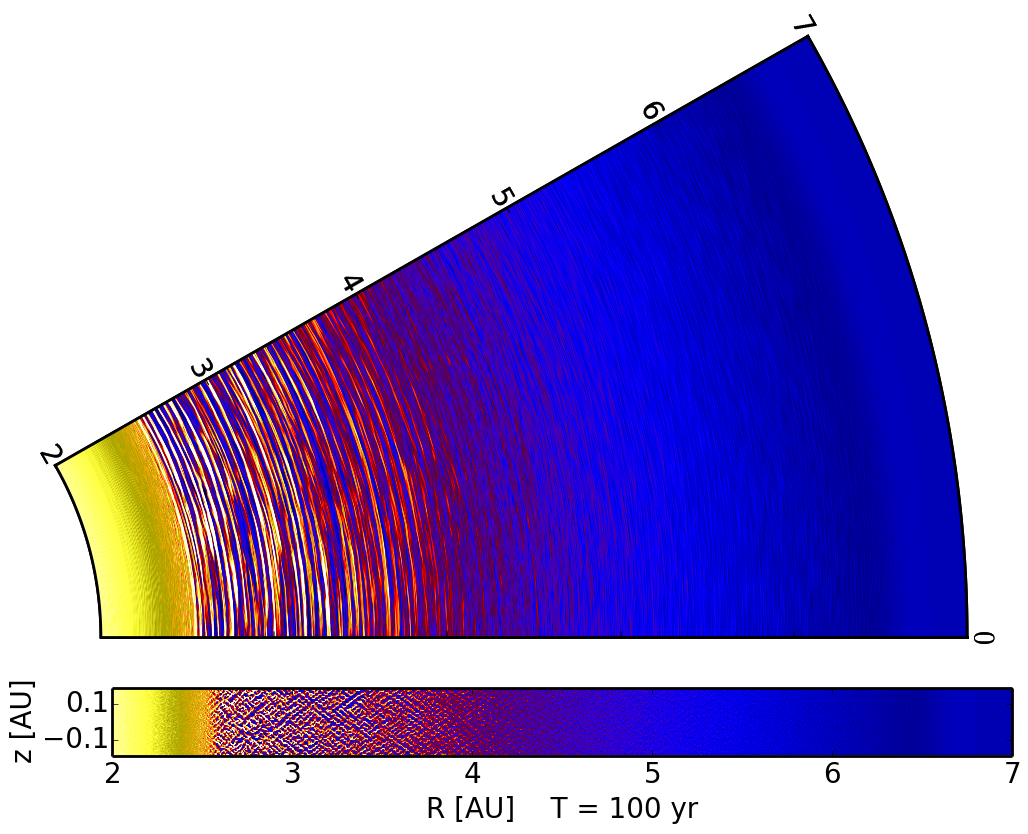
\includegraphics[width=0.44\linewidth]{figures/slice_nosg_02} \\
   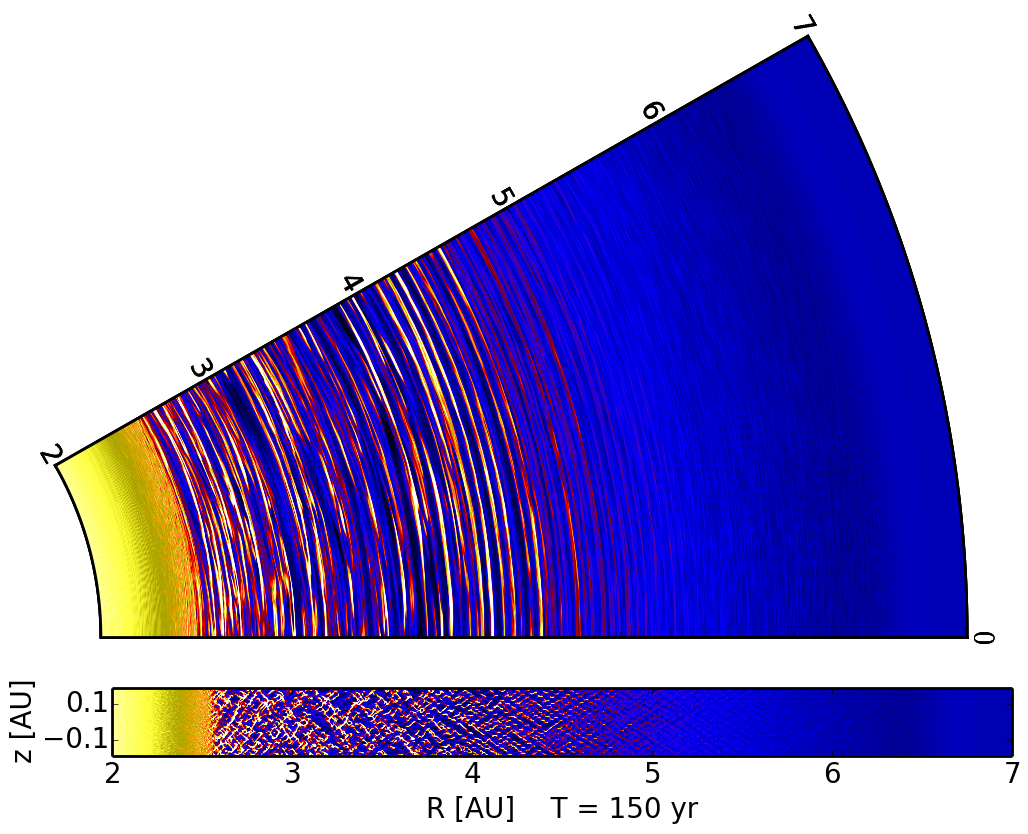
\includegraphics[width=0.44\linewidth]{figures/slice_nosg_03}
   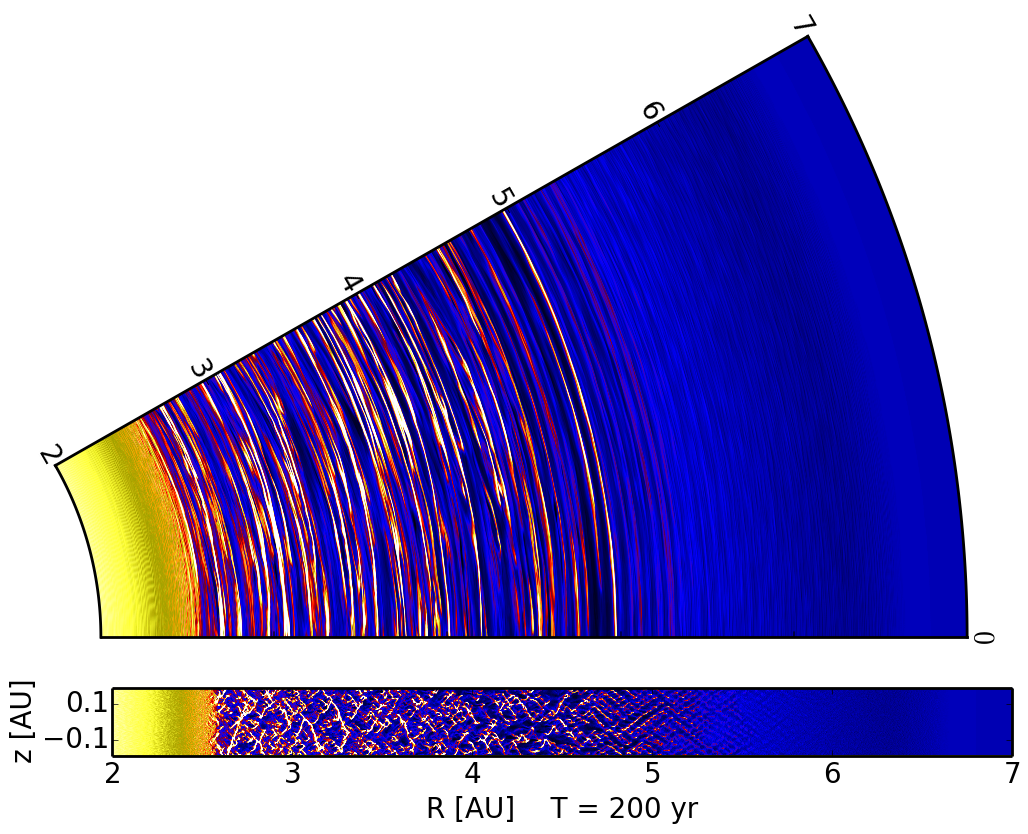
\includegraphics[width=0.44\linewidth]{figures/slice_nosg_04} \\
   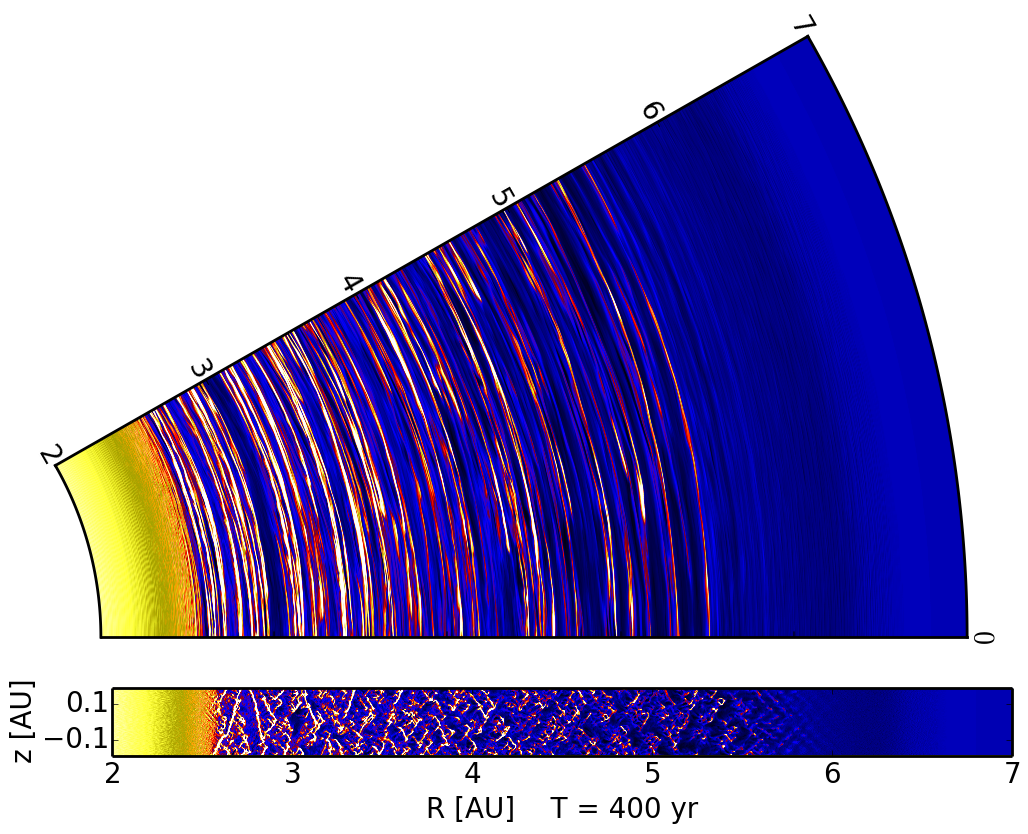
\includegraphics[width=0.44\linewidth]{figures/slice_nosg_05}
   \caption{
      Migawki z~symulacji BD3d obrazujące gęstość pyłu w~cięciach w
      płaszczyznach $R -\varphi$ oraz $R - z$ przechodzących przez środek 
   domeny obliczeniowej, dla czasów $T= 50, 100, 150, 200, 400$}
   \label{fig:slicenosg}
\end{figure}
%
\par Obraz niestabilności strumieniowej diametralnie się zmienia po
uwzględnieniu samograwitacji pyłu. Początkowo ewolucja przebiega wzdłuż tego
samego scenariusza, dominujące mody niestabilności strumieniowej formują
charakterystyczny wzór--kratkę (Rysunek~\ref{fig:slicesg}). Tempo tworzenia się
zagęszczeń w~tej fazie $(50 - 100\yr)$ jest takie samo jak w~przypadku bez
samograwitacji~(Rysunek~\ref{fig:modes3d}). Ponadto dominujące mody lokują się
na mapie stabilności w~obszarze o największym tempie wzrostu wynikającyc z
liniowej analizy (Rysunek~\ref{fig:map3d}).  Pierwsza zauważalną różnicą jest
przekroczenie przez pył gęstości na której wcześniej niestabilność strumieniowa
się wysycała (por. środkowy panel na Rysunku~\ref{fig:hists}). Jest to prostą
konsekwencją faktu, że każde formujące się zagęszczenie jest dodatkowo
wspomagane działającą do wewnątrz siłą samograwitacyjną. Po $150$~latach dysk
pyłowy staje się dużo bardziej pofragmentowany w~kierunku azymutalnym.
Odstępstwo od osiowej symetrii jest wyraźnie zauważalne. Warstwy gęstego pyłu na
skutek wzajemnego oddziaływania grawitacyjnego (jak i~własnego ciężaru)
zaczynają się deformować coraz silniej zmieniając swoją strukturę w~kierunku
azymutalnym. W~ciągu kolejnych $50$~latach samograwitacja ,,ściska'' praktycznie
cały pył do jednej płaskiej warstwy w~płaszczyźnie $R - \varphi$ w~formie
długich pofalowanych włókien (Rysunek~\ref{fig:projs}). W~toku dalszej ewolucji
włókna fragmentują na mniejsze związane grawitacyjnie obiekty -- planetezymale,
które podlegają dalszym oddziaływaniom dynamicznym. 

%
\begin{figure}
   \centering
   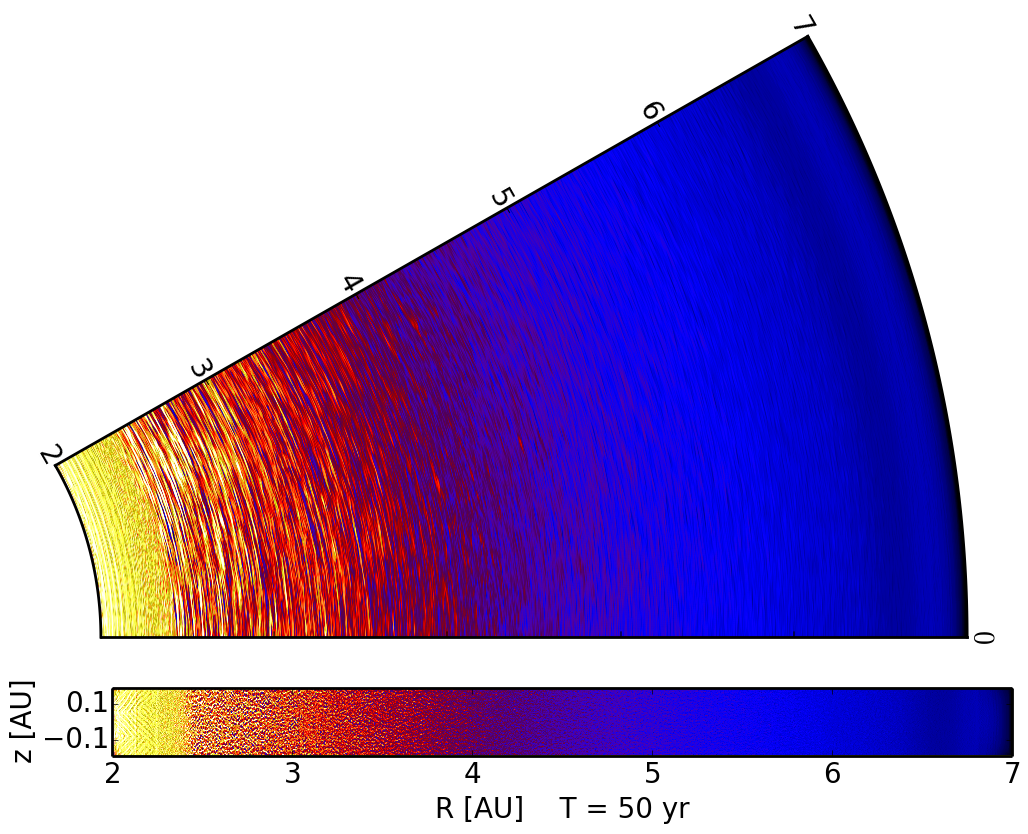
\includegraphics[width=0.44\linewidth]{figures/slice_sg_01}
   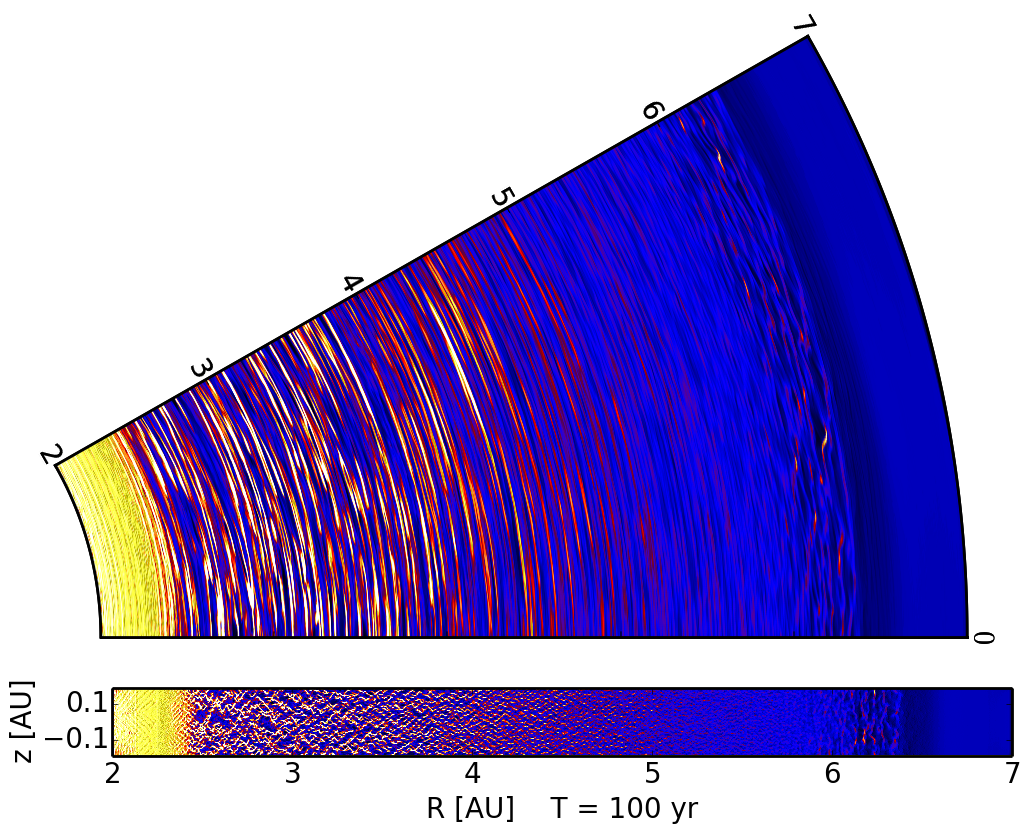
\includegraphics[width=0.44\linewidth]{figures/slice_sg_02} \\
   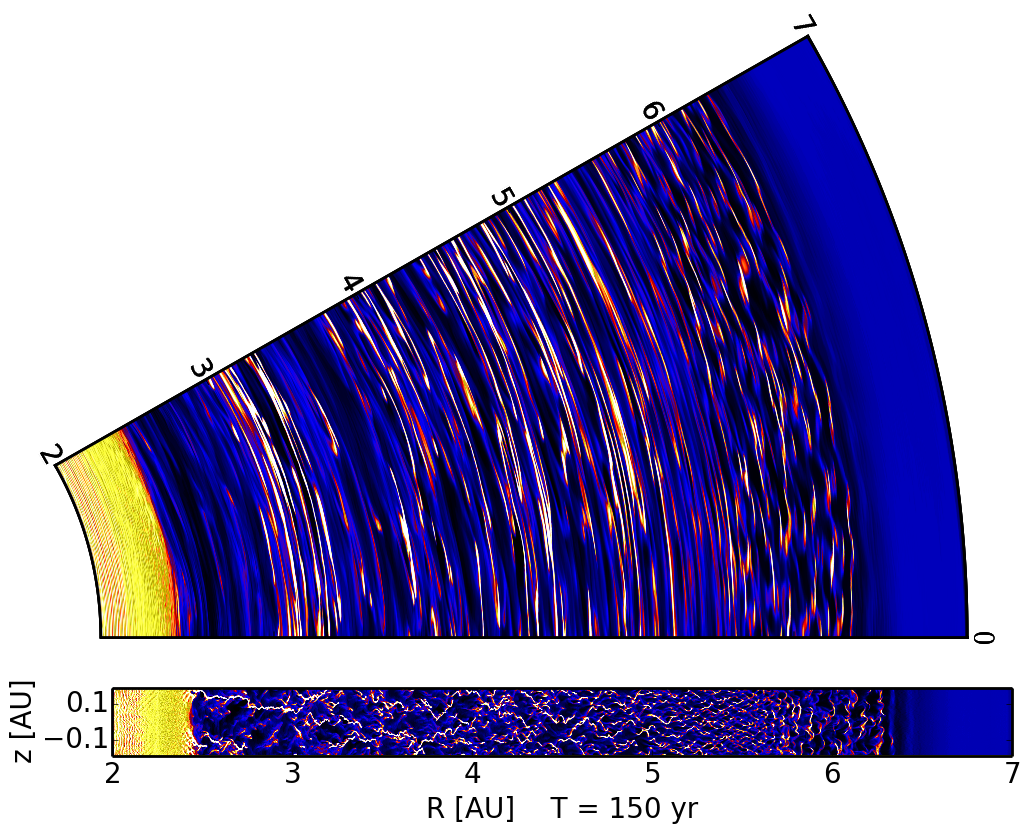
\includegraphics[width=0.44\linewidth]{figures/slice_sg_03}
   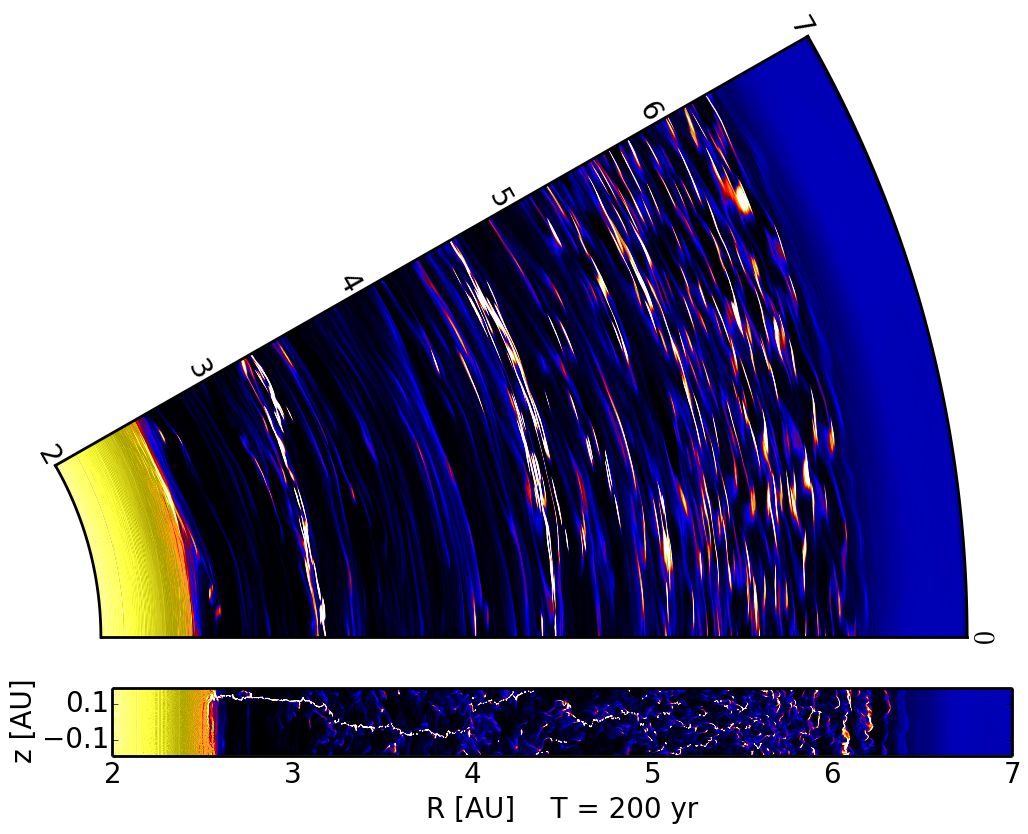
\includegraphics[width=0.44\linewidth]{figures/slice_sg_04} \\
   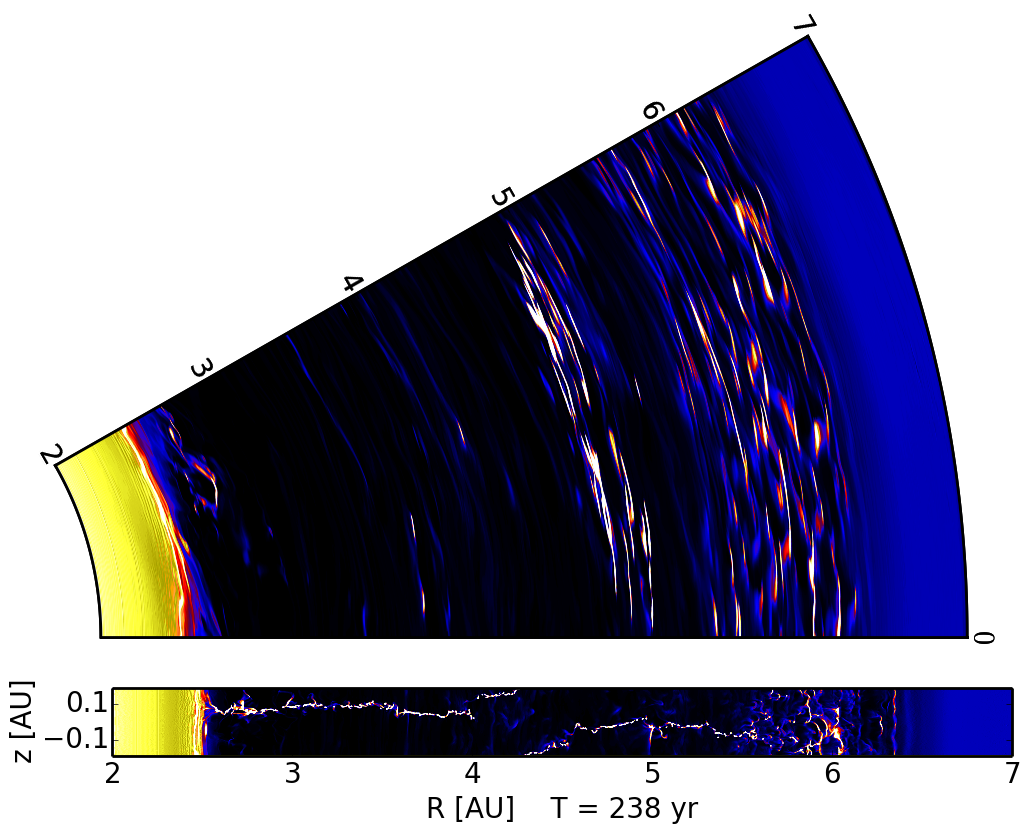
\includegraphics[width=0.44\linewidth]{figures/slice_sg_05}
   \caption{
      Migawki z~symulacji BD3dS obrazujące gęstość pyłu w~cięciach w
      płaszczyznach $R -\varphi$ oraz $R - z$ przechodzących przez środek 
   domeny obliczeniowej, dla czasów $T= 50, 100, 150, 200, 250$}
   \label{fig:slicesg}
\end{figure}
%
\par Wpływ samograwitacji na ewolucję układu dobrze obrazuje zestawienie
histogramów masy pyłu w~funkcji promienia orbitalnego i~gęstości pyłu
(Rysunek~\ref{fig:hists}). Dla symulacji BD3d, pomimo osiągnięcia przez nią
lokalnie zagęszczeń o $1\div1.5$ rzędów większych niż początkowy rozkład,
większość masy pyłu jest równomiernie rozłożona pomiędzy gęstościami $10^{-11}
\div 5\cdot10^{-10}\g\cm^{-3}$. W~połączeniu obrazem wyłaniającym się z~cięć
przez domenę obliczeniową, sugeruje to krótki czas życia zagęszczeń i
nieustający przepływ masy pomiędzy obszarami o niskiej i~wysokiej gęstości.
Natomiast w~symulacji BD3dS rozkład masy jest zgoła inny. Po osiągnięciu
granicznej wartości gęstości $\sim10^{-9}\g\cm^{-3}$ masa zaczyna ,,uciekać'' w
kierunku maksymalnej gęstości. Wytwarza się rozkład potęgowy opadający w
kierunku rzadszych obszarów, z~wyraźnym gwałtownym obcięciem na wartości
granicznej gęstości $\sim10^{-8}\g\cm^{-3}$.
%
\begin{figure} 
  \centering
  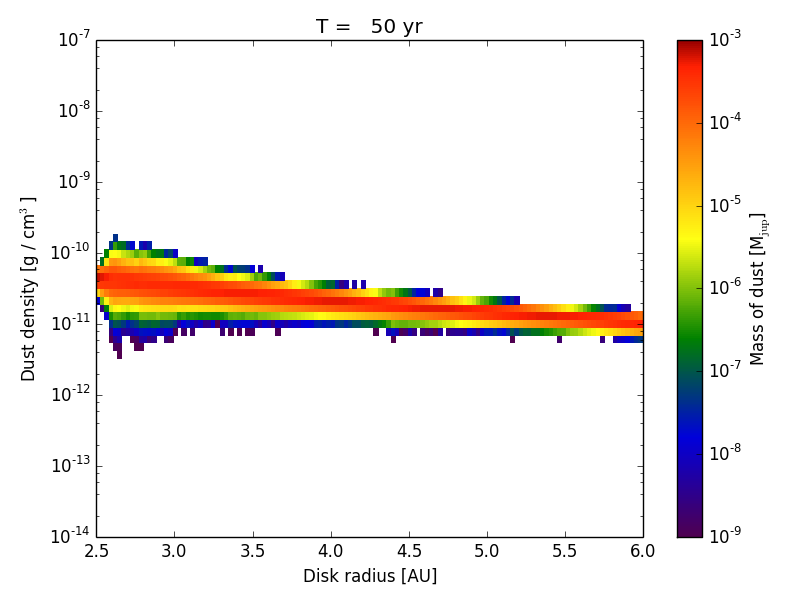
\includegraphics[width=0.4\linewidth]{figures/hist2d_nosg_01.png}
  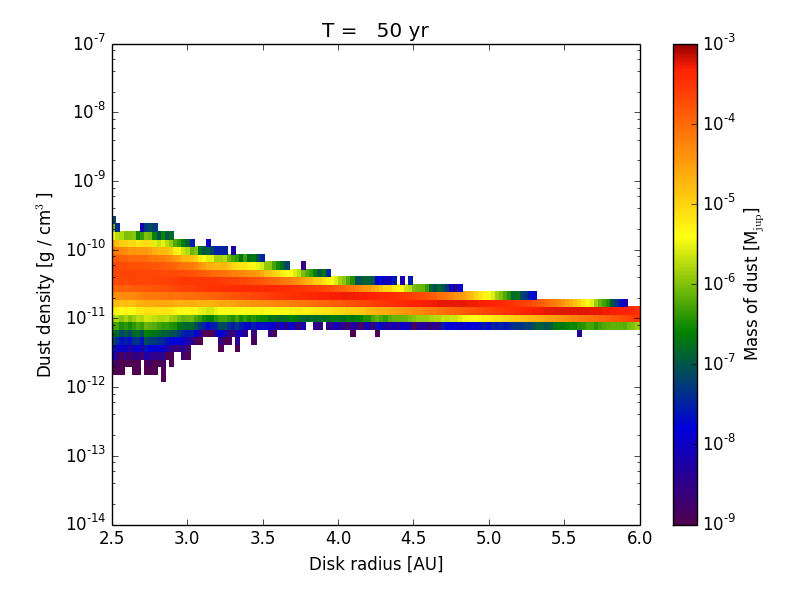
\includegraphics[width=0.4\linewidth]{figures/hist2d_sg_01.png} \\
  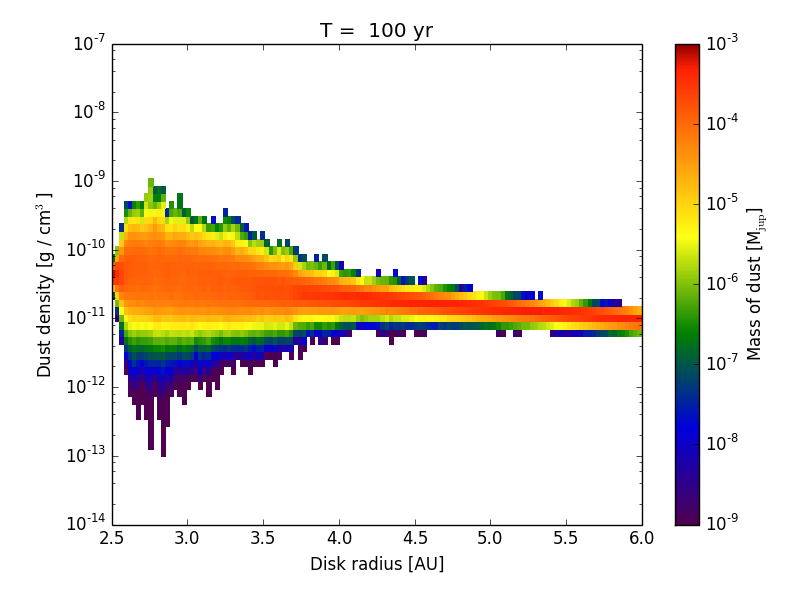
\includegraphics[width=0.4\linewidth]{figures/hist2d_nosg_02.png}
  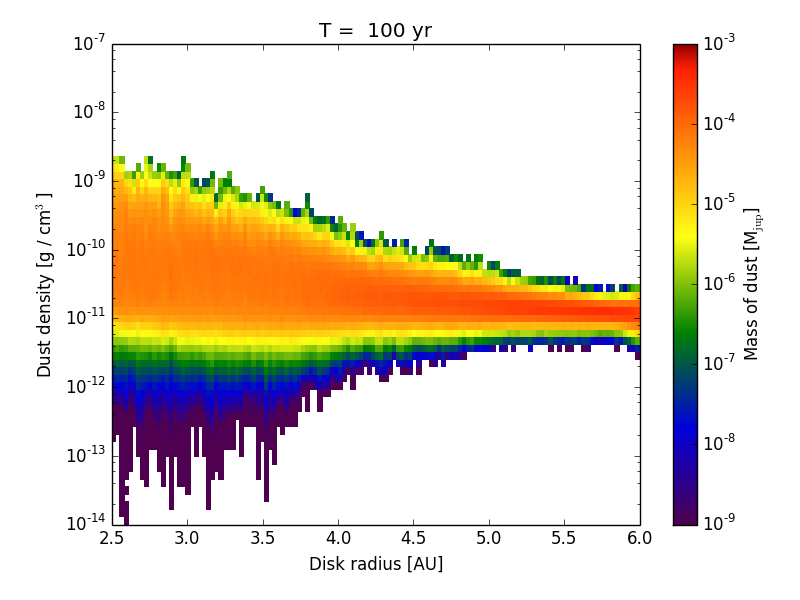
\includegraphics[width=0.4\linewidth]{figures/hist2d_sg_02.png} \\
  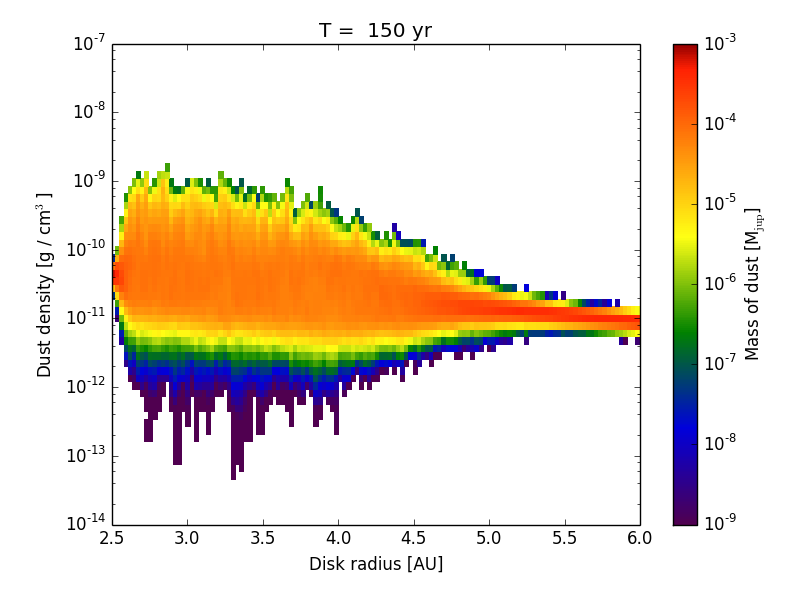
\includegraphics[width=0.4\linewidth]{figures/hist2d_nosg_03.png}
  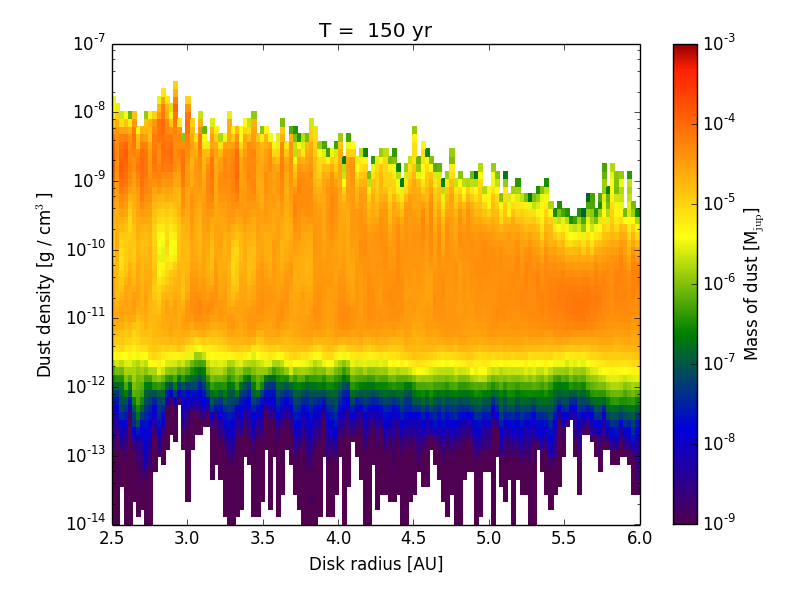
\includegraphics[width=0.4\linewidth]{figures/hist2d_sg_03.png} \\
  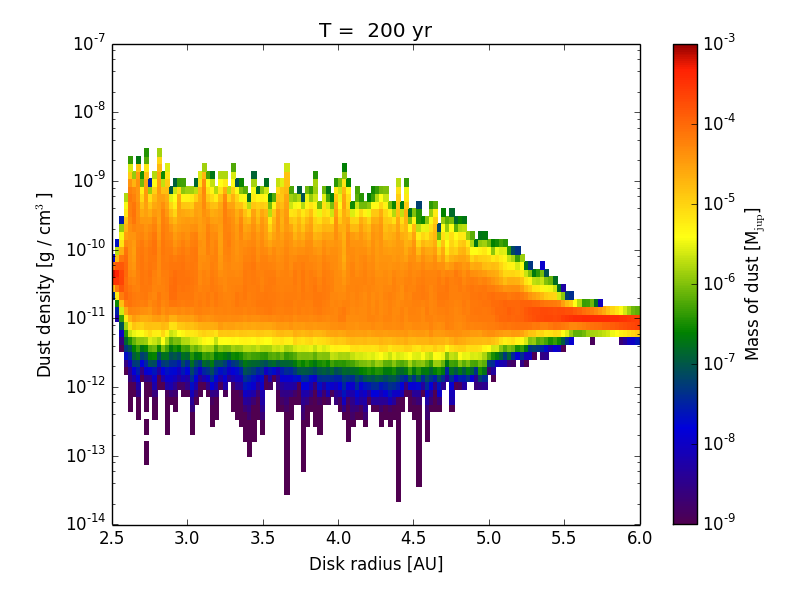
\includegraphics[width=0.4\linewidth]{figures/hist2d_nosg_04.png}
  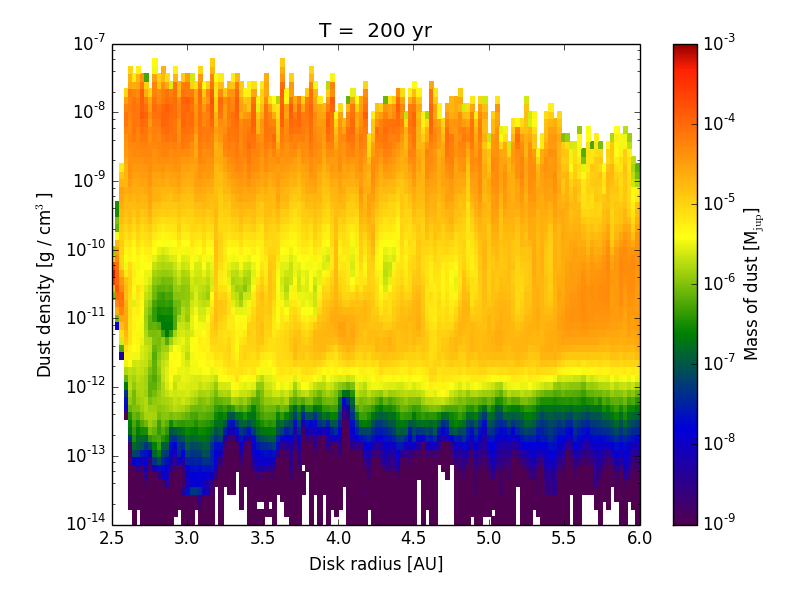
\includegraphics[width=0.4\linewidth]{figures/hist2d_sg_04.png} 
  \caption{Histogramy masy pyłu w~funkcji promienia i~gęstości pyłu, lewa
  kolumna bez samograwitacji, prawa kolumna z~samograwitacja}
  \label{fig:hists} 
\end{figure}
%
\par Histogram masy niestety nie daję informacji o kształcie i
charakterystycznych skalach obiektów w~których znajduje się większość masy pyłu,
ani nie pozwala stwierdzić czy pył jest grawitacyjnie związany. W~celu
rozszerzenia przeprowadzonej analizy zebrany materiał poddano procedurze
identyfikacji topologicznie powiązanych ze sobą komórek obliczeniowych
znajdujących się w~przedziale gęstości $10^{-10}\div10^{-8}\g\cm^{-3}$. W~tym
celu wykorzystano pakiet do analizy i~wizualizacji
danych~\yt{}~\footnote{Szczegółowe informacje na temat \emph{clump-finder'a}
można znaleźć w~rozdziale 7.7 w~pracy~\cite{yt}. Autor niniejszej pracy
rozszerzył pakiet \yt{} o możliwość czytania plików wynikowych z~kodu
PIERNIK, a także zaimplementował wsparcie dla współrzędnych cylindrycznych.}.
Uzyskanie informacji o topologii rozkładu gęstości pyłu jest pierwszym krokiem w
celu ustalenia, czy powstające zagęszczenia są w~stanie utworzyć grawitacyjnie
związane obiekty. Dla każdego zidentyfikowanego obiektu -- ,,clumpu'', można
określić relację pomiędzy jego energią kinetyczną, a studnią potencjału w~której
się znajduje. Kryterium związania można wyrazić przez

\begin{equation}
   \label{eq:bcrit}
   E_{\textrm{kin}} \equiv \sum\limits_{i=1}^N \frac{m_i\tilde{\mathbf{v}}_i^2}{2} 
   < \sum\limits_{i=1}^N m_i\tilde{\Phi}_i \equiv E_{\textrm{pot}},
\end{equation}
gdzie $N$ to liczba komórek obliczeniowych wchodzących w~skład clumpu, $m_i$,
$\tilde{\mathbf{v}}$, $\Phi_i$ to odpowiednio masa pyłu, prędkość w~układzie
środka masy clumpu, potencjał wynikający z~samograwitacji w~poszczególnej
komórce. Potencjał samograwitacyjny został uzyskany bezpośrednio z~PIERNIKa jako
rozwiązanie równania Poissona~\mref{eq:poisson} dla gęstości sumarycznej obu
składników płynowych. Ze względu na gładki rozkład gęstości gazu, jego
kontrybucję można było wyeliminować poprzez odjęcie od potencjału
samograwitacyjnego w~każdej komórce obliczeniowej wartości średniej z~tego
potencjału dla każdej orbity
\begin{equation}
   \tilde{\Phi}_i(R,\varphi,z) = \Phi_i(R,\varphi,z) -
   \left<\Phi_i\right>_{z\varphi}(R).
\end{equation}
%
Przy obliczaniu energii kinetycznej clumpu, poza przejściem z~prędkością do układu środka
masy w~celu uwzględnienia wpływu rotacji obłoku na jego kontrakcję, dodatkowo
wzięto pod uwagę możliwy wpływ turbulencji, która nie jest opisywana przyjętym
modelem
\begin{equation}
   \label{eq:ekin}
   \tilde{\mathbf{v}}_i = \mathbf{v}_i - \frac{\sum m_i \mathbf{v}_i}{\sum m_i}
   + \alpha c_s^2,
\end{equation}
gdzie wartość $\alpha$ ustalono na $0.05$. Zastosowanie
kryterium~\mref{eq:bcrit} dla każdego zidentyfikowanego obiektu, pozwoliło na
oszacowanie że ok. $19\%$ masy pyłu po czasie $T = 250\yr$ skupiła się w~formie
grawitacyjnie związanych obłoków. Na wynik ten ma wpływ dobór parametru $\alpha$
ze względu na postać równania energii kinetycznej~\mref{eq:ekin}. Dla $\alpha <
0.05$ wyraz wynikający z~turbulentnego transportu momentu pędu staje się
zaniedbywalny i~nie zmienia liczby związanych obłoków pyłu. Dla $\alpha = 0.1$
związana masa pyłu spada do $\sim 9\%$ całkowitej masy.  Szczegółowy histogram
mas wszystkich zidentyfikowanych obiektów ($\alpha = 0.05$) został przedstawiony
na Rysunku~\ref{fig:masshist}.

\begin{figure}
   \centering
   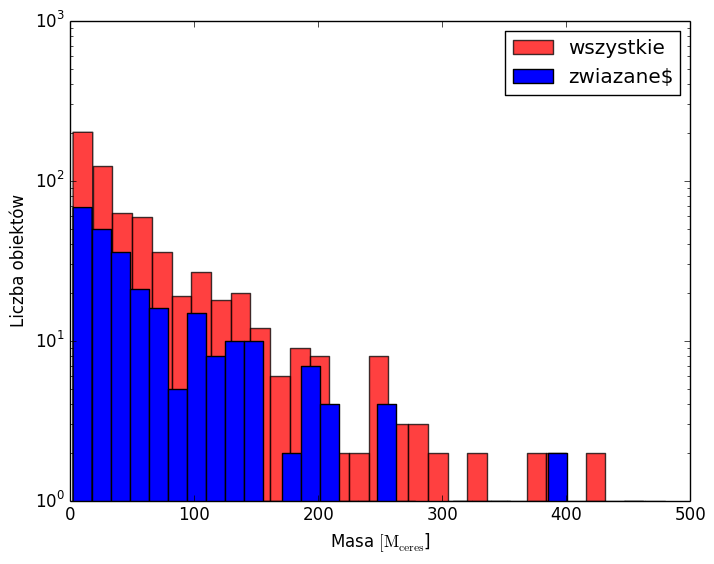
\includegraphics[width=0.49\linewidth]{figures/masshist.png}
   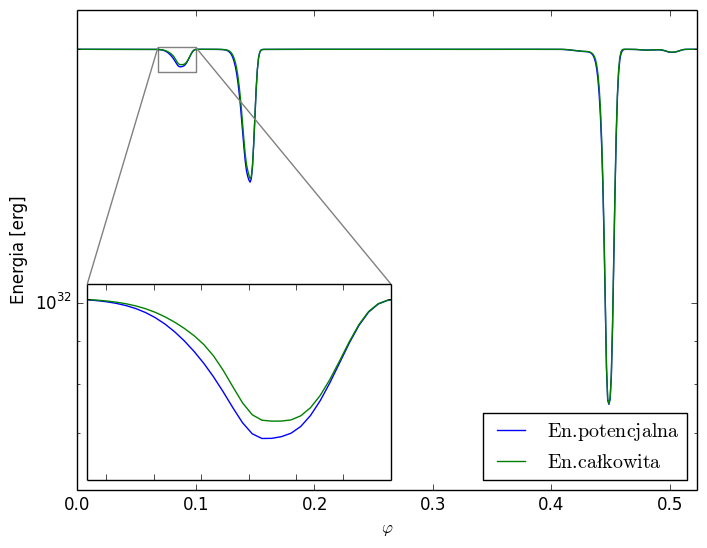
\includegraphics[width=0.49\linewidth]{figures/energie.png}
   \caption{(Lewy panel) Histogram przedstawiający rozkład masy w~topologicznie powiązanych
   obiektach istniejących w~domenie obliczeniowej dla symulacji BD3dS dla czasu
   $T=250\yr$. Kolorem niebieskim zaznaczono clumpy związane grawitacyjnie, zaś
   kolorem czerwonym wszystkie obiekty.
   (Prawy panel) Przekrój azymutalny przez domenę obliczeniową dla $R=3.84\AU$
   i~$z=0.01\AU$ dla czasu $T=250\yr$ pokazujący energię potencjalną (zgodnie z
   definicją w~równaniu~\mref{eq:bcrit}) oraz sumę energii potencjalnej i~energii
   kinetycznej dla danego clumpu.}
   \label{fig:masshist}
\end{figure}
%
\begin{figure}
   \centering
   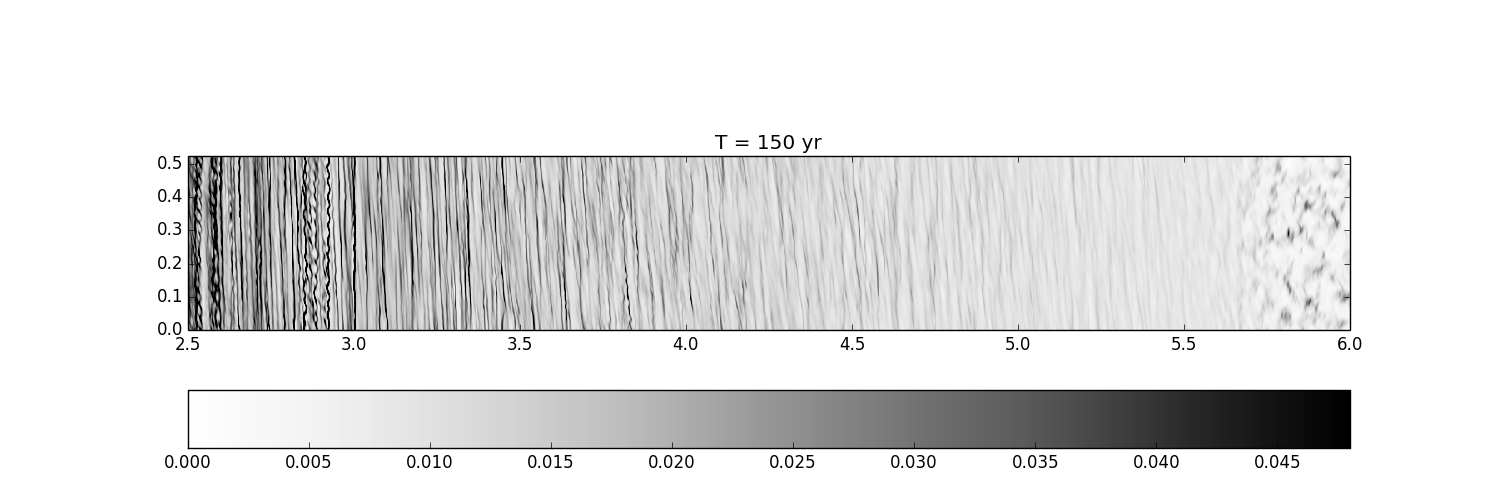
\includegraphics[width=0.95\linewidth]{figures/proj1.png}\\
   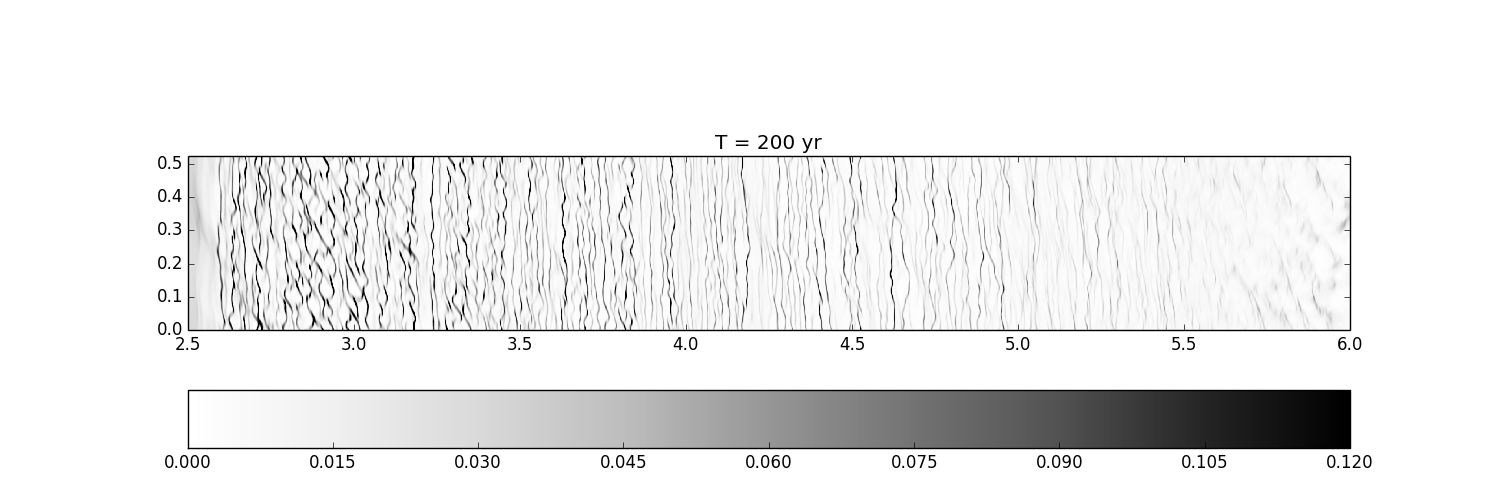
\includegraphics[width=0.95\linewidth]{figures/proj2.png}\\
   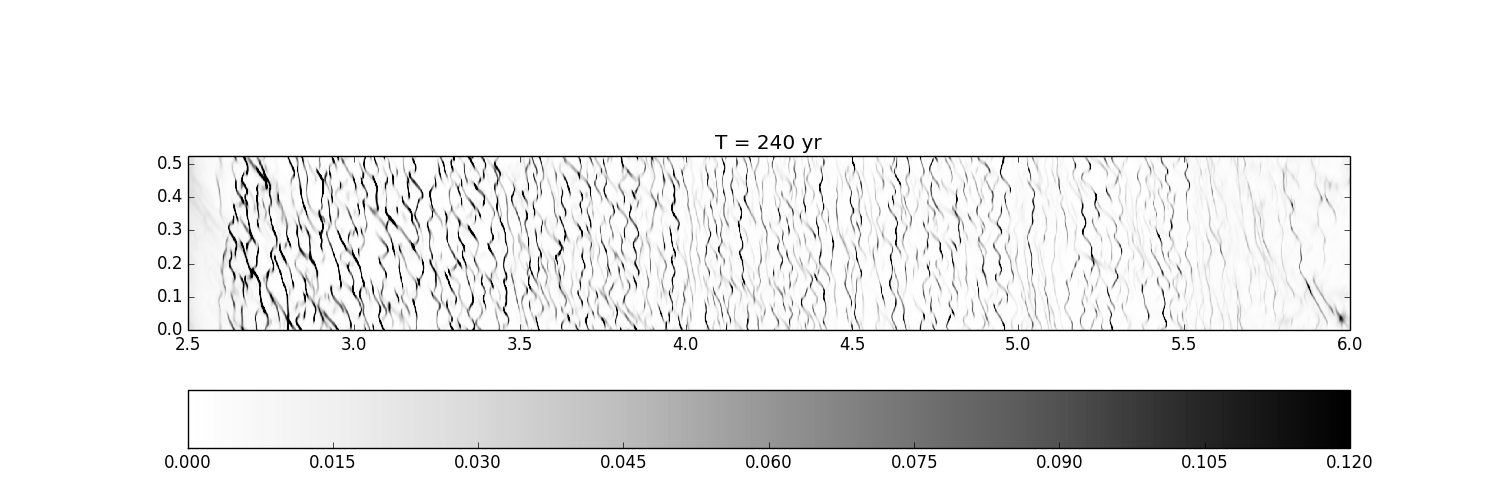
\includegraphics[width=0.95\linewidth]{figures/proj3.png}
   \caption{Gęstość
      kolumnowa pyłu w~symulacji BD3dS dla czasu $T=150, 200, 250\yr$}
   \label{fig:projs}
\end{figure}
%
\begin{figure}
   \centering
   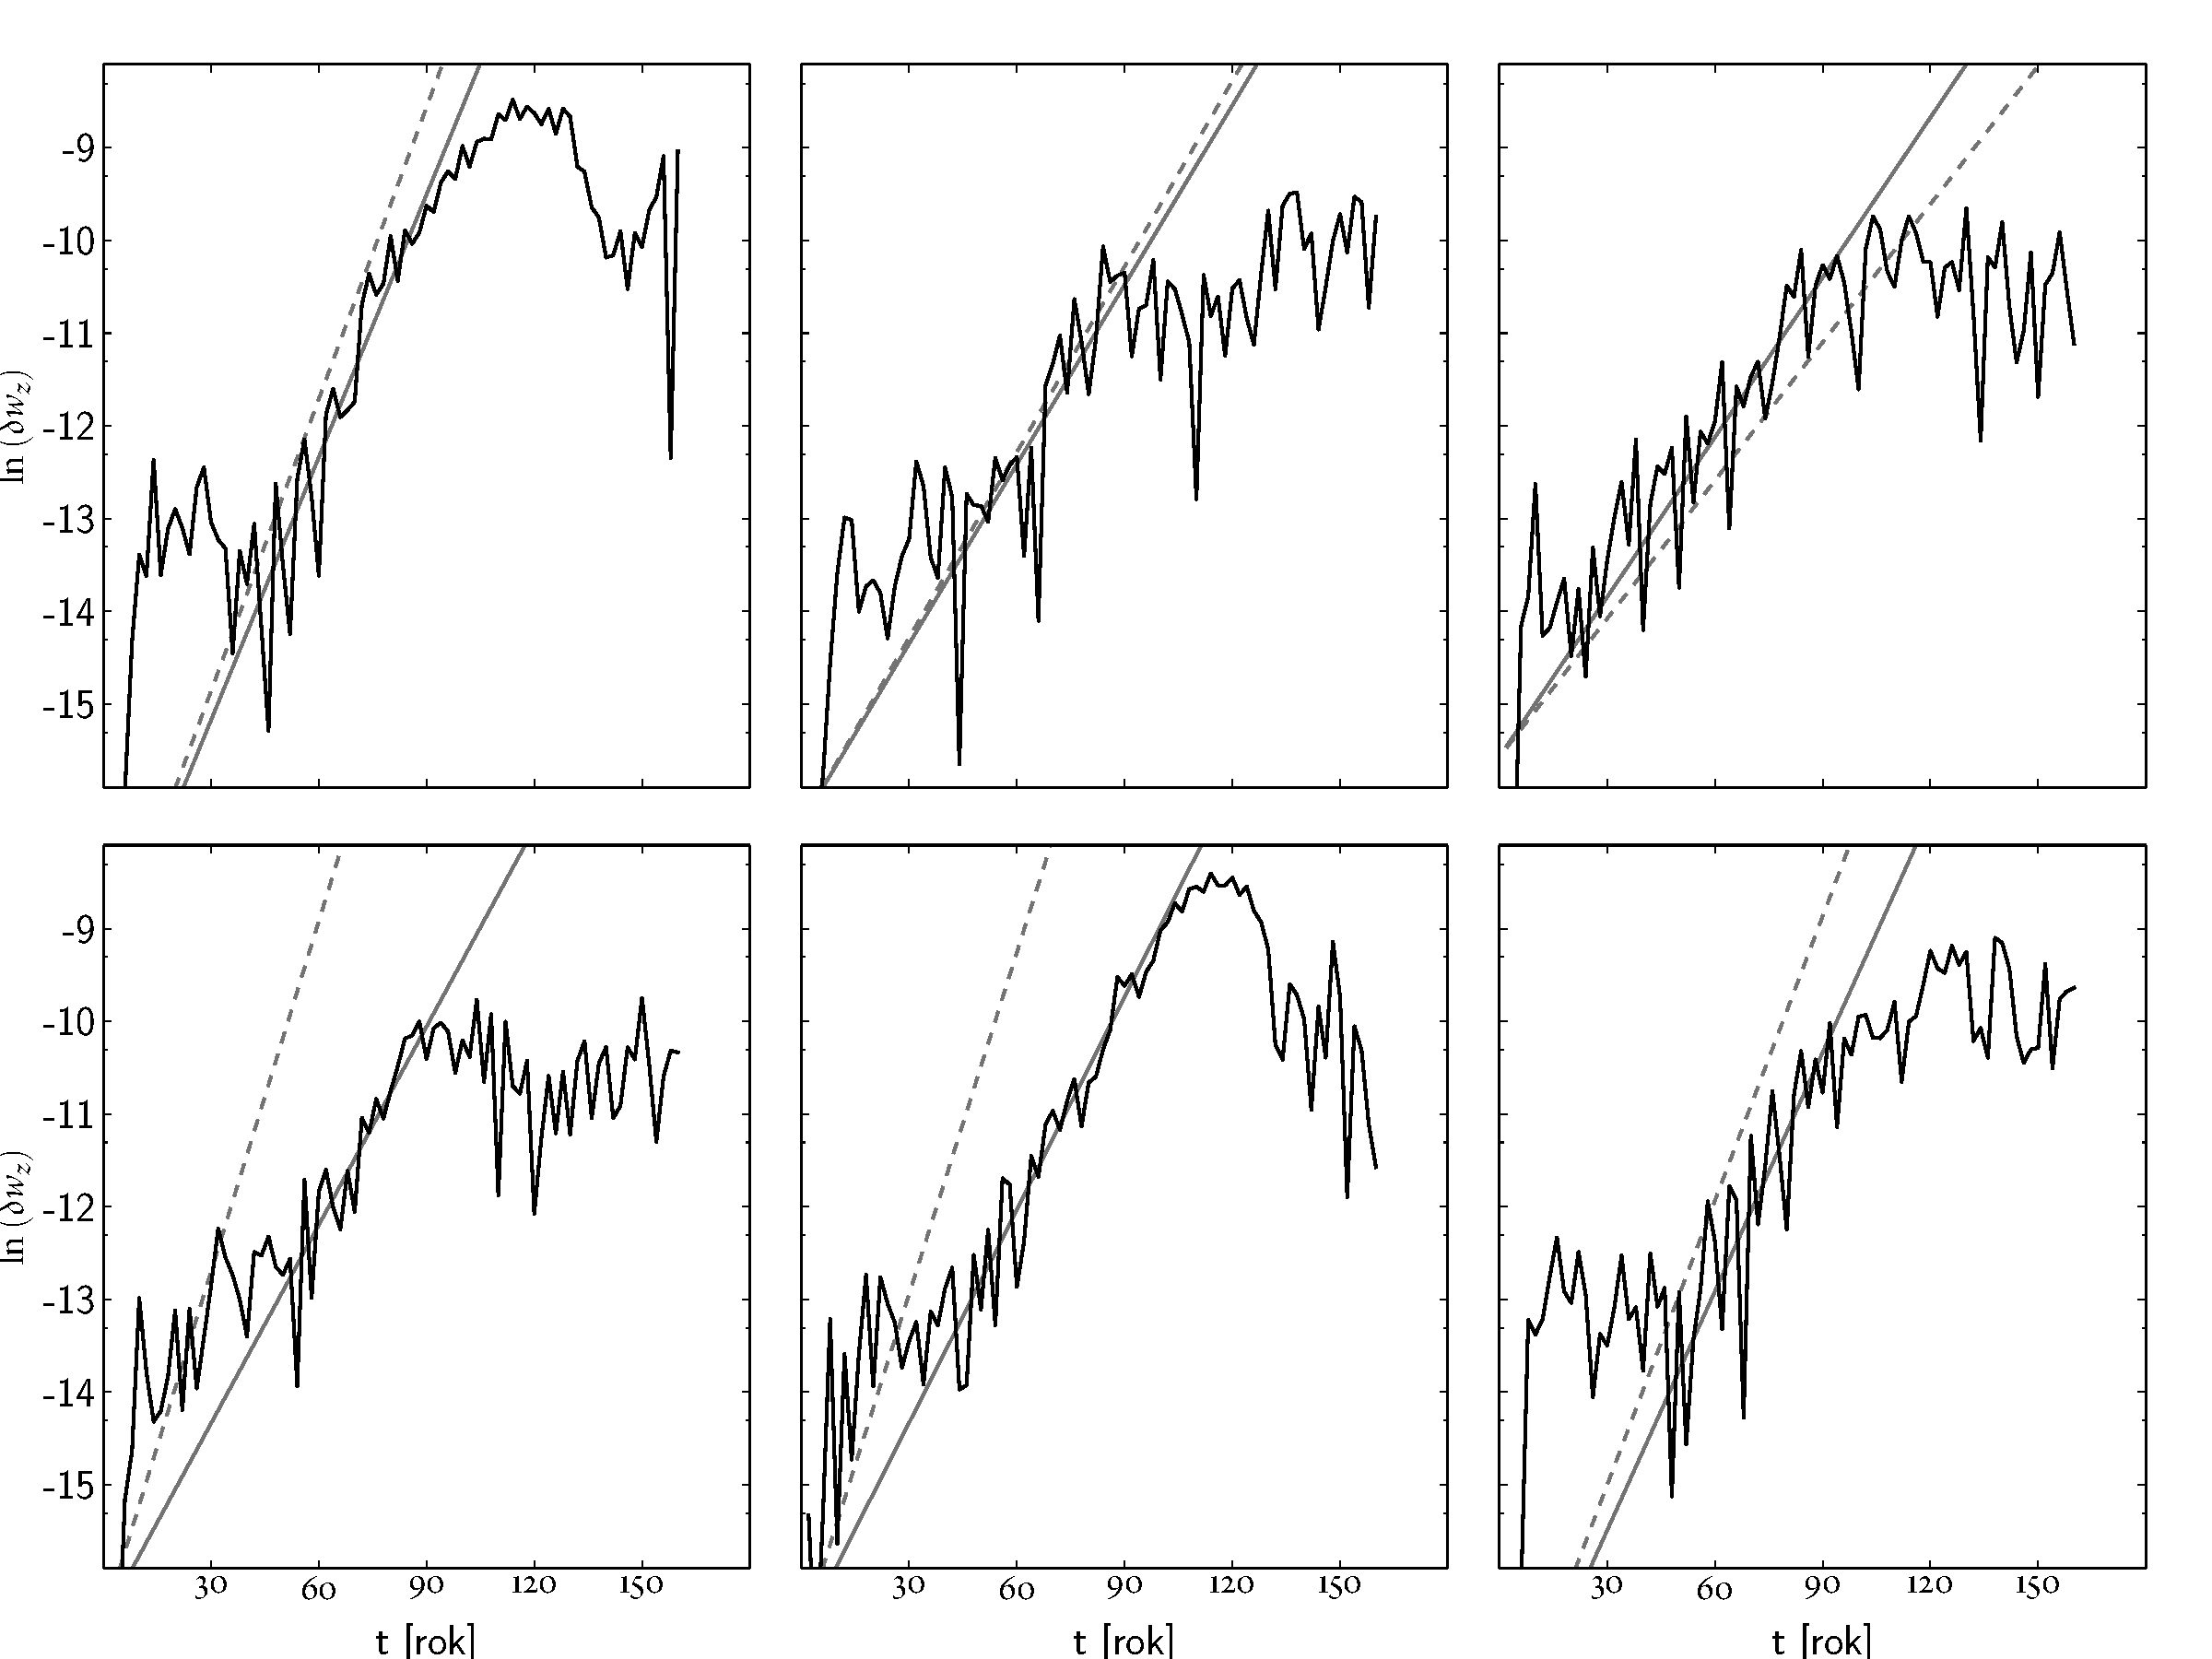
\includegraphics[width=0.95\linewidth]{figures/nosg_vlzd_growth}
   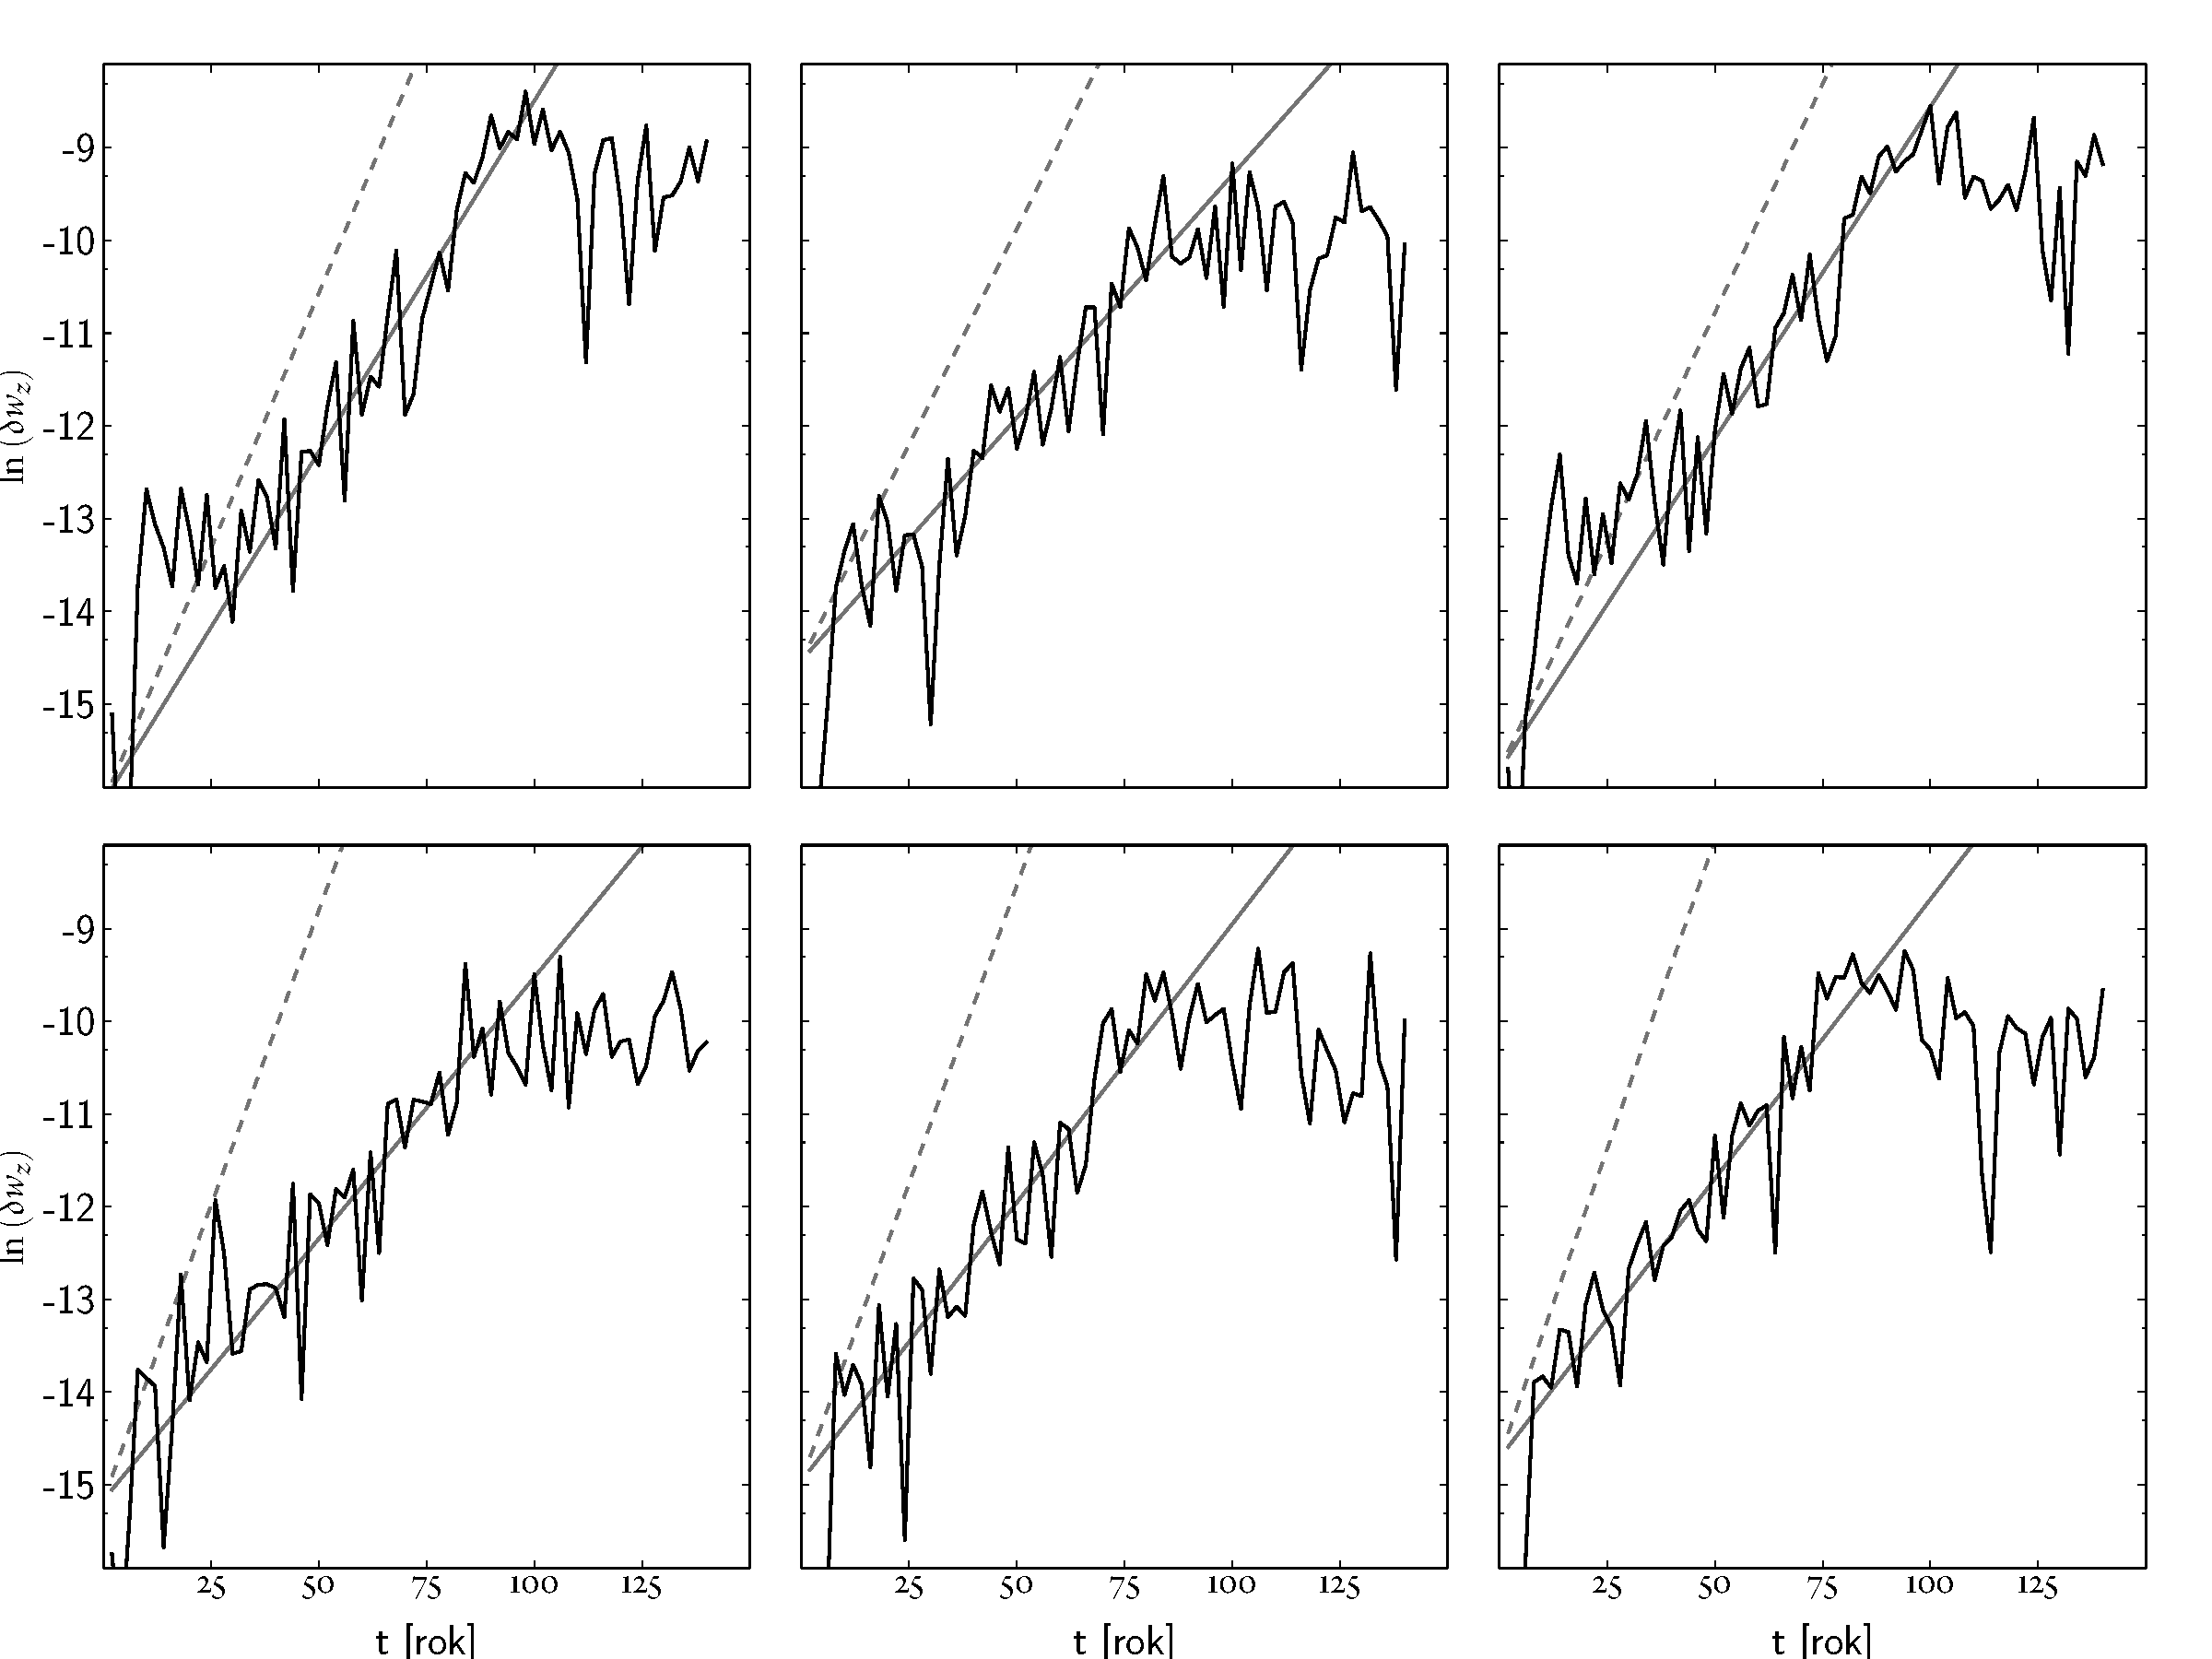
\includegraphics[width=0.95\linewidth]{figures/sg_vlzd_growth}
   \caption{6 dominujacych modów z~BD3d i~BD3dS}
   \label{fig:modes3d}
\end{figure}
%   
\begin{figure}
   \centering
   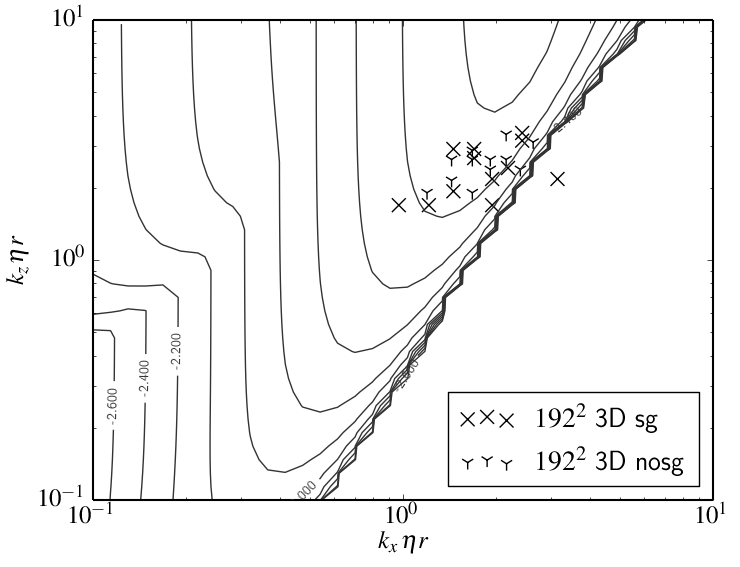
\includegraphics[width=0.5\linewidth]{figures/3d_map_x3_50.png}
   \caption{Mapa stabilności BD3d i~BD3dS}
   \label{fig:map3d}
\end{figure}
% x3_50n.png
% vim: tw=80 ts=3: 

\begin{savequote}[75mm]
   Va'esse deireádh eap eigean$\ldots$
\qauthor{Saga o wiedźminie, Andrzej Sapkowski}
\end{savequote}

\chapter{Dyskusja i plany na przyszłość}
Przedmiotem rozważań zaprezentowanych w niniejszej pracy jest niestabilność
strumieniowa wynikająca z oddziaływania pyłu i gazu w dysku protoplanetarnym z
udziałem i bez udziału samograwitacji. Przedstawione w poprzednich rozdziałach
wyniki opierają się na serii symulacji numerycznych fragmentu dysku
protoplanetarnego w dwu i trzech wymiarach oraz liniowej analizy stabilności
wykonanej dla przypadku dwuwymiarowego.
%
%Przy czym
%zaniedbano pionową składową grawitacji od masy punktowej umieszczonej w centrum
%układu współrzędnych.
%
W eksperymentach numerycznych przeprowadzonych dla ziaren pyłu o rozmiarach od
10 do 50$\cm$ zaobserwowano gwałtowny wzrost zaburzeń w gęstości i prędkości
pyłu o charakterystycznych długościach fali zgodnych z przewidywaniami lokalnej,
liniowej analizy stabilności takiego układu. Wcześniejsze symulacje numeryczne
innych autorów~\cite{YG05, JY07, TB09, BS10a, BS10b} opierały się na lokalnym
przybliżeniu kostki ścinanej. Prowadziło to do szeregu uproszczeń m.in.
traktowania globalnego, radialnego ciśnienia gazu jako stałego i niezmiennego
współczynnika~\cite{N86}, stosowania bezwymiarowego czasu zatrzymania przy
obliczaniu wzajemnego oddziaływania obu płynów~\cite{YG05}. Głównym
osiągnięciem niniejszej pracy jest rozszerzenie modelu stosowanego przez innych
autorów poprzez uwzględnienie pełnej dynamiki okołogwiazdowego dysku w kierunku
radialnym i wykazanie, że w takim przypadku dostępne algorytmy i zasoby
obliczeniowe umożliwiają wiarygodne modelowanie niestabilności
strumieniowej. Istotnym rozszerzeniem wcześniejszych modeli fizycznych było 
użycie właściwego prawa tarcia aerodynamicznego~\mref{eq:tauf}
zamiast przybliżonego rachunku opartego na stałym, bezwymiarowym czasie
zatrzymania. 
%
Przedstawiony model globalnego dysku jest rozwinięciem dotychczas
publikowanych modeli lokalnych. Należy jednakże podkreślić, że model zaprezentowany 
w niniejszej pracy opiera się na uproszczających założeniach do których należy
zaliczyć brak stratyfikacji, pominięcie pola magnetycznego skutkujące
brakiem niestabilności magnetorotacyjnej, uwzględnienie jednej tylko frakcji
aglomeratów pyłowych o wybranym rozmiarze oraz przeszacowanie początkowej masy
pyłu.
%
%Do jego największych wad można zaliczyć brak stratyfikacji oraz nieuwzględnienie
%wpływu globalnej turbulencji wywołanej niestabilnością
%magneto-rotacyjną~\cite{DKJ14}. 

%
\par Pierwszy etap niniejszej pracy opierał się na wykonaniu testów
zbieżnościowych dla różnych parametrów fizycznych dysku protoplanetarnego co
pozwoliło na określenie minimalnej liczby komórek obliczeniowych $(n\approx32)$
dla kodu \textsc{PIERNIK}, umożliwiającej na dokładne odwzorowanie liniowej fazy
wzrostu.  Otrzymane, we wszystkich przeprowadzonych eksperymentach numerycznych,
liczby falowe najszybciej rosnących modów niestabilności, a także ich położenia na
mapie stabilności ($s(k_x, k_z)$), są zgodne z przewidywaniami liniowej analizy
niestabilności strumieniowej i potwierdzają właściwy wybór użytych metod
numerycznych. Kolejnym krokiem było wykonanie symulacji trójwymiarowych bez
samograwitacji i porównanie ich wyniku z wcześniejszymi symulacjami
dwuwymiarowymi. Uzyskane wyniki pokazują iż trójwymiarowe symulacje odtwarzają w
pełni przebieg ewolucji niestabilności strumieniowej, zgodnie z przewidywaniami
liniowej analizy stabilności przeprowadzonej dla układu zredukowanego do dwóch
wymiarów. Finalnym etapem pracy było przeprowadzenie w pełni trójwymiarowej
symulacji dwuskładnikowego dysku protoplanetarnego z uwzględnieniem wpływu
samograwitacji. Należy podkreślić, że pomimo założenia dużo większej niż
kanoniczna wartości stosunku gęstości gazu do gęstości pyłu, symulowany dysk
jest początkowo stabilny zgodnie z kryterium Toomre'a~\mref{eq:toomre}.
Parametr $Q$ jest stały dla całej domeny obliczeniowej i wynosi około $40$
(rów.~\ref{eq:Qemp}). Wzbudzenie niestabilności strumieniowej prowadzi do
uformowania lokalnych zagęszczeń pyłu, których gęstość jest nawet stukrotnie
większa niż gęstość początkowa pyłu. Ilość zgromadzonej lokalnie masy pyłu
przekracza granicę stabilności grawitacyjnej i w rezultacie w układzie formuje
się znaczna liczba związanych grawitacyjnie obiektów, które należy interpretować
jako zalążki planetezymali. Zgromadzona w tych obiektach materia
pyłowa reprezentuje $50\cm$ aglomeraty pyłowe, a ich całkowita masa jest
wystarczająca aby po ,,sprasowaniu'' na skutek grawitacji powstały zwarte ciała o
rozmiarach rzędu setek kilometrów. Dzięki temu połączone działanie
niestabilności strumieniowej i niestabilności grawitacyjnej skutkuje pokonaniem
\emph{metrowej bariery wzrostu} aglomeratów pyłowych o którym była mowa w
rozdziale~\ref{sec:paradigm}.
%
\par 
Oceniając przydatność przedstawionego modelu należy pamiętać o zastosowanych
przybliżeniach. Głównym niedostatkiem modelu jest przeszacowany początkowy
stosunek gęstości pyłu do gęstości gazu. Dla przypomnienia jest on ponad
stukrotnie wyższy niż wartość kanoniczna~\cite{FS03} typowa dla ośrodka
międzygwiazdowego. Jak pokazują przedstawione w rozdziale~\ref{sec:sim_2d}
wyniki symulacji dwuwymiarowych, niższy stosunek gęstości pyłu do gęstości gazu
wydłuża tempo wzrostu niestabilności strumieniowej, dlatego modelowanie
niestabilności strumieniowej jest  dużo trudniejsze i bardziej kosztowne
obliczeniowo.  Jednakże całkowita masa pyłu zawarta w domenie obliczeniowej o
rozpiętości 1/6 pełnego kąta azymutalnego wynosi około $35\Mearth$ i co do rzędu
wielkości odpowiada masie skalistych planet i jąder planet gazowych Układu
Słonecznego. Biorąc pod uwagę, że użyty w symulacjach radialny profil gęstości
MMSN jest tylko \emph{dolnym ograniczeniem} rzeczywistego rozkładu gęstości
materii w dysku protoplanetarnym, to przedstawiony w niniejszej pracy model
ciągle pozostaje zgodny z antycypowanymi warunkami początkowymi dla Układu
Słonecznego~\cite{D07}.
\par Przewidywania teorii ,,akrecji na jądra'' istotnie zależą od procesu
odpowiedzialnego za formowanie się planetezymali~\cite{HBP13}. Początkowa
funkcja masy planetezymali nie jest dobrze określona. Przyjmuje się, że ma
postać funkcji potęgowej, bądź złożenia dwóch funkcji potęgowych~\cite{R03}.
Wyniki przedstawione w rozdziale~\ref{sec:sim_3d} pozwalają określić spektralny
rozkład masy zgromadzonej w grawitacyjnie związanych obiektach, stanowiących
zgodnie z przyjętym modelem zalążki planetezymali.  Zakładając, że rozkład masy
grawitacyjnie związanych obiektów pyłowych jest dany funkcją:
%
\begin{equation}
   f(m) \propto m^{-a},
\end{equation}
%
w rozdziale~\ref{sec:sim_3d} dopasowano do otrzymanego rozkładu masy funkcję o
wykładniku $a = 1.25\pm0.12$. Wykładnik ten mieści się w zakresie przewidywanym
przez innych
autorów~\cite{R03}, którzy szacują jego wartość między $1$ a $3$. Ponadto prawy
skraj funkcji masy (Rysunek~\ref{fig:massfun} można opisać funkcją o wykładniku
$a$ w przedziale $2 < a < 3$ który jest zbieżny z wynikami symulacji N-ciałowych
formowania się planet~\cite{MFFK98}.  Należy jednak zauważyć, iż przedstawiona
na rysunku~\ref{fig:massfun} funkcja masy utworzonych w symulacji grawitacyjnie
związanych obiektów może być obarczona sporymi błędami systematycznymi.
W szczególności lewy skraj jest ograniczony poprzez skończoną rozdzielczość
siatki obliczeniowej: typowe rozmiary obiektów związanych grawitacyjnie wynoszą
od kilkudziesięciu do kilkuset komórek, co przekłada się na rozmiar liniowy
obiektów związanych grawitacyjnie rzędu kilku komórek obliczeniowych. Jest to
wielkość wysoce niewystarczająca do poprawnego odwzorowania niestabilności
grawitacyjnej w takim obiekcie.  Prawy skraj natomiast, zawiera mało
reprezentatywną statystycznie liczbę obiektów.
%
\par Typowe rozmiary otrzymanych w symulacji BD3dS grawitacyjnie związanych
zagęszczeń mieszczą się w przedziale $10^{11} \div 10^{12}\cm$ i są one spójne z
charakterystykami obiektów, które mogą tworzyć zwarte planetezymale w toku
dalszej ewolucji~\cite{HS08}. Średnie końcowe gęstości pyłu nie są niestety
miarodajne ze względu na przypuszczalny wpływ ograniczonej rozdzielczości siatki
obliczeniowej. Należy jednak mieć na uwadze, że dodatkową niepewności dotycząca
liczby powstających obiektów wprowadza podskalowa turbulencja sparametryzowana
współczynnikiem $\alpha$ występującym w kryterium związania
grawitacyjnego\mref{eq:ekin}.
%Jak pokazano w rozdziale~\ref{sec:sim_3d} dla
%$\alpha = 0.1$ masa pyłu zgromadzona w związanych grawitacyjnie obiektach
%stanowi tylko $5\%$ całej masy pyłu obecnej w dysku.  Jednakże oczekiwane
%wartości $\alpha$ w dyskach protoplanetarnych oscylują wokół wartości
%$0.01$~\cite{FD11}, dla których efektywnie związana w obiektach masa stanowi
%ponad $15\%$ całkowitej masy pyłu w dysku.
W rozdziale~\ref{sec:sim_3d} oszacowano, że wybór parametru $\alpha$ w
niewielkim stopniu zmienia kryterium grawitacyjnego związania obiektów pyłowych.
Dalszym krokiem pozwalającym na rozwinięcie przedstawionego w niniejszej pracy
modelu dysku protoplanetarnego powinno być uwzględnienie rzeczywistego źródła
turbulencji w dysku, np. poprzez rozszerzenie modelu o wpływ pola magnetycznego
i uwzględnienie skutków niestabilności magnetorotacyjnej. Podobnie wprowadzenie
stratyfikacji w dysku pozwoliłoby na uwzględnienie wpływu niestabilności
Kelvina-Helmholtza.  Niezbędne jest także zwiększenie rozdzielczości siatki
obliczeniowej w obszarach, które podlegają niestabilności grawitacyjnej. Byłoby
to możliwe dzięki zastosowaniu zaimplementowanego niedawno w kodzie
\textsc{PIERNIK} mechanizmu \emph{adaptywnej siatki obliczeniowej}\footnote{ang.
\emph{Adaptive Mesh Refinement}}. Pozwoliłoby to dokładniej śledzić proces
kolapsu grawitacyjnego i zdecydowanie poprawić oszacowanie uzyskiwanej
początkowej funkcji masy obiektów grawitacyjnie związanych.  Mimo tego, że
zastosowanie techniki siatek adaptywnych może efektywnie zwiększyć rozdzielczość
liniową siatki obliczeniowej o parę rzędów wielkości, to śledzenie w dysku
rozciągającym się na wiele jednostek astronomicznych obiektów których rozmiary
nie przekraczają setek kilometrów, nadal nastręcza spore trudności.  Naturalnym
krokiem w takiej sytuacji jest rozszerzenie algorytmu numerycznego o tzw.
,,cząstki pochłaniające''\footnote{ang. \emph{,,sink particles''}}. ,,Cząstki
pochłaniające'' są punktami materialnymi, które oddziałują z otaczającym je
płynem tylko poprzez siły grawitacji i pochłaniają płyn znajdujący się wewnątrz
zadanego promienia akrecji zwiększając swoją masę~\cite{FBCK10}. Wprowadzenie
,,cząstek pochłaniających'' do przedstawionych w niniejszej pracy symulacji
pozwoliłoby m.in. na określenie tempa akrecji masy na związane grawitacyjnie
obiekty, co przy użytych dotychczas metodach numerycznych nie było możliwe.
Niezmiernie ważne jest również wydłużenie czasu trwania symulacji tak, aby
możliwe było uwzględnienie efektów migracji formujących się, grawitacyjnie
związanych obiektów~\cite{ML14}.

%\par Rozszerzenie może iść w dwie strony: bardziej realistyczny model dysku t.j.
%stratyfikacja~(Johansen ostatnie prace) i pole magnetyczne, rozwój
%algorytmiczny t.j. adaptywna siatka niezbędna do śledzenia zapadania się
%obłoku, podskalowy model ewolucji pyłu np.  metodami MC~(Aska)


%%%%%%%%%%%%%%%%%%%%%%%%%%%%%%%%%%%%%%%%%%%%%%%%%%%%%%%%%%%%%%%%%%%%%%%%%%%%%%%%
% vim: tw=80 ts=3: 

%\begin{savequote}[75mm]
%\qauthor{Edward Mallory, The Difference Engine by William Gibson and Bruce
%   Sterling}
%\end{savequote}

\chapter{Podsumowanie}

Głównym osiągnięciem niniejszej pracy jest potwierdzenie hipotezy, że w globalnym
dysku gazowo--pyłowym, w którym oba składniki są traktowane jako płyn, zasadniczą
rolę w
powstawaniu gęstych obiektów pyłowych odgrywa niestabilność strumieniowa. 
Istotnym osiągnięciem jest również stwierdzenie, że niestabilność
strumieniowa w globalnym dysku gazowo--pyłowym, w obecności samograwitacji
materii, może prowadzić do wytworzenia się grawitacyjnie związanych obiektów.
Zebrany w niniejszej pracy materiał oparty na symulacjach numerycznych
pozwala stwierdzić, że:

\begin{itemize}
   \item zarówno dwu- jak i trójwymiarowe symulacje quasi--globalnego dysku
      gazowo--py\-ło\-we\-go, w którym oba wzajemnie ze sobą oddziałujące poprzez siłę
      tarcia składniki są traktowane w przybliżeniu płynowym, stanowią wiarygodne
      narzędzie do badania niestabilności strumieniowej;
   \item algorytmy numeryczne zaimplementowane w kodzie \textsc{Piernik}
      pozwalają na odtworzenie z wystarczającą dokładnością liniowej fazy
      wzrostu niestabilności strumieniowej;
   \item niestabilność strumieniowa prowadzi do wytworzenia się w gazowo--pyłowym
      dysku obszarów, w których gęstość pyłu jest ponad stukrotnie wyższa niż
      maksymalna początkowa gęstość pyłu;
   \item niestabilność strumieniowa z uwzględnieniem samograwitacji materii
      prowadzi do wytworzenia się populacji związanych grawitacyjnie, pyłowych
      obiektów o spektralnym rozkładzie masy danym funkcją potęgową o wykładniku
      $-1.25\pm0.12$;
   \item masa pyłu zgromadzona w pojedynczych, grawitacyjnie związanych obiektach
      odpowiada ciałom o rozmiarach rzędu kilkudziesięciu do kilkuset
      kilometrów;
   \item całkowita masa pyłu zgromadzona w grawitacyjnie związanych obiektach w
      przedstawionym modelu 
      jest wystarczająca do wytworzenia pojedynczego jądra gazowego
      olbrzyma, bądź dwóch lub trzech planet skalistych;
   \item dalsze prace nad modelem są potrzebne w celu uściślenia ilościowych
      szacunków całkowitej masy, liczby i spektrum masowego powstających
      planetezymali.
\end{itemize}
Zebrane w niniejsze pracy wyniki stanowią przyczynek do wyjaśnienia
kontrowersji tzw. \emph{metrowej bariery} w modelu akrecji na
jądra. Pomimo pewnych idealizacji i uproszczeń, obecnych w użytym modelu, praca
stanowi istotny krok na przód w kierunku zrozumienia procesów
prowadzących do powstawania planet.

%%%%%%%%%%%%%%%%%%%%%%%%%%%%%%%%%%%%%%%%%%%%%%%%%%%%%%%%%%%%%%%%%%%%%%%%%%%%%%%%
% vim: tw=80 ts=3: 


\singlespacing

% the back matter
\clearpage
\bibliography{references}
\addcontentsline{toc}{chapter}{Bibliografia}
\bibliographystyle{plainnat}
%\include{endmatter/colophon}

\end{document}
